
\documentclass[acmtweb]{acmsmall}

\usepackage{amsfonts}	
\usepackage{enumerate,array}
\usepackage{algorithmicx}
\usepackage{algorithm2e}
\usepackage{multirow}	
\usepackage{graphicx}
\usepackage{color}

\newtheorem{principle}{Principle}
\def\network{{\sf N}}

\newcommand{\tuple}[2] {\langle #1,#2\rangle}

\acmVolume{1}
\acmNumber{1}
\acmArticle{1}
\acmYear{2013}
\acmMonth{8}


\begin{document}
\markboth{Qian and Adal{\i}}{Foundations of Trust and Distrust in Networks: Extended Structural Balance Theory}

\title{Foundations of Trust and Distrust in Networks: Extended Structural Balance Theory~\footnote{Note: A preliminary version of
    this paper appears in PST2013 under title ``Extended Structural
    Balance Theory for Modeling Trust in Social Networks''}}

\author{
Yi Qian
\affil{Department of Computer Science, Renssealer Polytechnic Institute}
Sibel Adal{\i}
\affil{Department of Computer Science, Renssealer Polytechnic Institute}
}

\begin{abstract}
Modeling trust in very large social networks is a hard problem due to
the highly noisy nature of these networks that span trust
relationships from many different contexts, based on judgments of
reliability, dependability and competence. Furthermore, relationships
in these networks vary in their level of strength. In this paper, we
introduce a novel extension of structural balance theory as a
foundational theory of trust and distrust in networks. Our theory
preserves the distinctions between trust and distrust as suggested in
the literature, but also incorporates the notion of relationship
strength which can be expressed as either discrete categorical values,
as pairwise comparisons or as metric distances. Our model is novel,
has sound social and psychological basis, and captures the classical
balance theory as a special case. We then propose a convergence model,
describing how an imbalanced network evolves towards new balance and
formulate the convergence problem of a social network as a Metric
Multidimensional Scaling (MDS) optimization problem.  Finally, we show
how the convergence model can be used to predict edge signs in social
networks, and justify our theory through extensive experiments on real
datasets.
\end{abstract}


\category{H.3.1}{Content Analysis and Indexing}{}
\category{H.3.3}{Information Search and Retrieval, Relevance Feedback}{}
\category{J.4}{Social and Behavioral Sciences}{}

\terms{Algorithms, Measurement, Performance}

\keywords{Trust, Distrust, Social Networks, Structural Balance}

\acmformat{Yi Qian and Sibel Adal{\i}, 2013.  Foundations of Trust and
  Distrust in Networks: Extended Structural Balance Theory.}

\begin{bottomstuff}
Research was sponsored by the Army Research Laboratory and was
accomplished under Cooperative Agreement Number W911NF-09-2-0053. The
views and conclusions contained in this document are those of the
authors and should not be interpreted as representing the official
policies, either expressed or implied, of the Army Research Laboratory
or the U.S. Government. The U.S. Government is authorized to reproduce
and distribute reprints for Government purposes notwithstanding any
copyright notation here on.


Author's addresses: 
Yi Qian, , Department of Computer Science, Renssealer Polytechnic Institute, 110 8th St., Troy NY, 12180;
Sibel Adal{\i}, Department of Computer Science, Renssealer Polytechnic Institute, 110 8th St., Troy NY, 12180.
\end{bottomstuff}

\maketitle


\section{Introduction}
Modeling trust in very large social networks is a hard problem due to
the highly noisy nature of these networks. These networks span trust
relationships from many different contexts, based on judgments of
reliability, dependability and
competence~\cite{Adali:2013}. Furthermore, trust relationships vary in
their level of strength as participants may or may not know each other
well. These relationships change over time and only a subset of the
existing relationships are declared explicitly in a given dataset.
One specific problem of interest is inferring new relationships and
making recommendations based on existing relationships. To this date,
many algorithms for such prediction problems are based on machine
learning methods. These methods generate multiple structural features
from the known relationships, and then use these features to classify
the unknown
relationships~\cite{golbeck:distrust2011}\cite{Guha:04}\cite{Leskovec:2010}. In
particular, the concept of structural balance is widely applied when
developing these algorithms. For example, Leskovec et al. generate a
class of ``triad features'' in their prediction algorithm, i.e. a pair
of relationships constraining a third
relationship~\cite{Leskovec:2010}. They also use the structural
balance as a touchstone to see the congruence between their practical
results and the long studied theory. In essence, the transitivity of
trust and distrust within a triad can be easily inferred from the
balance theory. Other algorithms~\cite{golbeck:distrust2011} make use
of similar assumptions without explicit mention of balance theory in
which trust and distrust relationships are mapped to metric distances
on a continuous range. While these algorithms show strong prediction
performance, there is no underlying theory that explains how
structural balance can be mapped to metric distances. That is, a
theory that stands as the cornerstone of trust prediction is
missing. Without such a theory, it is not possible to develop
principled algorithms and study to which degree a specific network
conforms to the theory, and to illustrate the importance of various
balance related properties of networks. Furthermore, in today's
networks in which individuals interact with a large number of others,
one expects that the relationships and their trust level will vary
considerably. As a result, it is not clear how Cartwright-Harary's
balance theory~\cite{Cartwright:56} can be applied to large scale
social networks in which nodes may have different types of trust and
distrust relationships, ranging from strong to weak.

In this paper, we  address all these concerns and make the following
unique contributions.
\begin{itemize}
\item We introduce a new extended balance theory that allows
  arbitrary relationship strengths. We express balance with two simple
  principles that preserve the meanings of trust and distrust:
  positive and negative trust relationships. We show how balance can
  be modeled when the strength of relationships are represented with either
  discrete categorical values, pairwise comparisons or metric
  distances using the same principles. Our novel method has sound
  social and psychological basis, and captures the classical balance
  theory as a special case.

\item We define the convergence model that describes precisely how an
  imbalanced network evolves towards new balance. The assumption
  behind our model is that in resolving tensions within imbalanced
  relationships, people tend to avoid the effort of changing
  relationships if possible. The introduction of extended balance
  theory allows us to formulate the convergence problem of a social
  network as a Metric Multidimensional Scaling (MDS) optimization
  problem.  We show how the convergence model can be used to predict
  edge signs in social networks by applying stress
  majorization~\cite{Gansner:05}. We introduce an efficient algorithm
  for sparse networks that can be applied to large networks.

\item We illustrate the convergence theory and our algorithmic
  solution on stylized networks. We show that neutral edges may become
  positive or negative edges based on the triads the edge is part
  of. Then, we show that the theory captures trust transitivity along
  positive paths naturally. The influence of a positive edge
  attenuates along long paths, even though all the edges overall
  remain positive. Finally, we show that as a node is part of more
  triads, the more it is effected by the relationships. All these
  results illustrate that our solutions follow the principles
  introduced by our theory.

\item We justify our theory through an extensive experimental study on
  three real datasets. Our method consistently outperforms the state
  of the art. In particular, improvement of our method over the state
  of the art is even more significant in networks with a larger
  proportion of negative edges. In such networks, it becomes
  increasinly crucial to capture the true meaning of negative
  edges. We show that we can achieve far superior prediction for
  strong trust edges, represented as bi-directional edges with the
  same sign. We illustrate the validity of our method with external
  data. We show that strong edges correspond to different rating
  behavior in Epinions for both trust and distrust. Additionally,
  whenever our algorithm predicts a distrust edge will change its sign
  after convergence, we show that the ratings for those edges actually
  increase more than average. Our algorithm is able to capture the
  expected change in ratings due to structural constraints. Finally,
  we show that our method can provide a promising first step towards
  solving the harder {\it link prediction
    problem}~\cite{Kleinberg:03}.
\end{itemize}

The remainder of this paper is organized as follows. In Section 2, we
describe the classical structural balance theory. We summarize the
related work in trust prediction and its relation to the balance
theory. Then, in Section 3, we describe our theory for structural
balance. We show how to incorporate relation strength into the
structural balance definition while preserving the basic principles of
balance. Section 4 defines the notion of convergence as an
optimization problem, how networks evolve towards a balanced state. We
show how the converged state of a network can be computed. We then
give an efficient algorithm for computing convergence approximately
for sparse graphs that disregards neutral edges~\footnote{The
  implementation of the sparse graph algorithm used in this paper is
  available as open source code at {\em
    github.com/rpitrust/structuralbalance}.}. Section 5 illustrates
convergence with the help of small stylized networks. Section 6
provides the setup of experiments involving three large networks that
are used in prior literature in trust prediction. We illustrate
different graphs that can be constructed from these networks to test
different hypotheses. In Section 7, we provide an extensive
experimental study of our algorithm, both comparing it to the state of
the art and also illustrating its various properties. Finally, we
conclude in Section 8 and discuss future work. 

\section{Structural Balance Theory \& Related Work} 
When modeling relationships between pairs of individuals, positive
relationships are representative of liking, loving, valuing or
approving someone, and negative relationships are representative of
disvaluing, disapproving or negatively valuing
someone~\cite{Cartwright:56}. Suppose we consider trust from the
perspective of trustworthiness where one trusts another if they are
considered to be truthful, to have integrity and to have positive
intentions towards the other. This definition of trustworthiness has a
definite affective component that can easily be considered as an
extension of the above definition. A positive relationship results in
trust because the other person is considered to have positive values
from the perspective of the trustor. Similarly, a negative
relationship results in distrust because the other person is
considered to have specific faults that would prevent them from being
trusted~\cite{Adali:2013}.

Trust and distrust are not symmetric constructs. A person who is not
trusted may eventually become trusted as a result of positive
evidence. However, a distrusted person may not be trusted even after
many positive experiences. As a result, one has to treat both types of
relationships differently. Note that often trust and distrust
relationships need not be mutual: A may trust B, but B may distrust A.
We will illustrate later with experiments on real networks that it is
possible to treat mutual trust relations as strong trust relations,
and the rest as weak trust. However, for now we will treat all trust
relations as simple undirected relationships.

\begin{figure}[th]
\centering
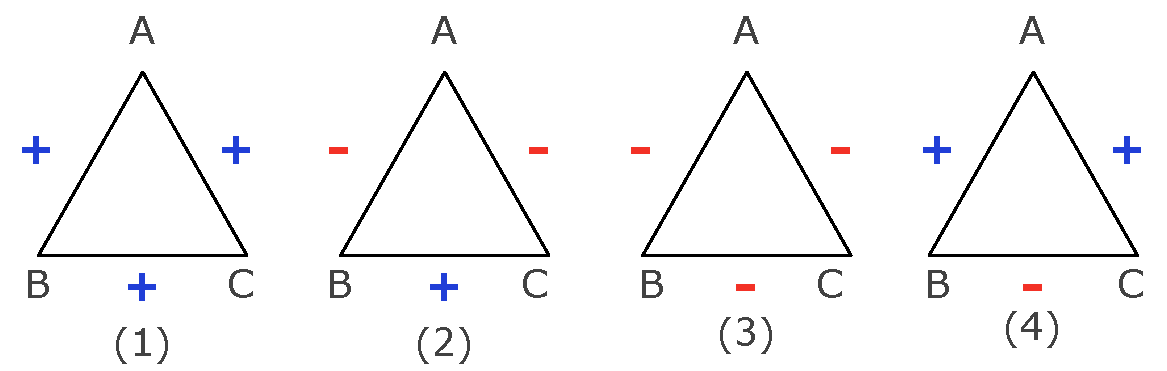
\includegraphics[height=0.8in]{strongBalance_ver.pdf}
\vspace*{-0.1in}
\caption{\label{fig:balance_strong}Classic structural balance with
  four different types of triads. In strong balance theory, triads 1,2
  are balanced and 3,4 are unbalanced. In weak balance theory, triads
  1,2 and 3 are balanced and 4 is unbalanced.}
\end{figure}

Structural balance theory (SBT) is based on the assumption that
certain types of relationships when viewed from a local perspective
are more natural for psychological reasons~\cite{kleinberg-book}. The
local level is defined as a triangle or triad consisting of
relationships between three people.  It is natural for three people to
be friends: Alice (A) is friends with Bob (B), Bob is friends with
Chris (C) and Chris is friends with Alice. This triangle (marked (1)
in Figure~\ref{fig:balance_strong}) is considered completely
positive. Similarly, a relation where two friends, Bob and Chris have
a common enemy Alice, is also natural (triangle (2) in
Figure~\ref{fig:balance_strong}). It is considered that in such
natural relationships, there is no tension in the
interactions. However, it is less natural for Alice and Bob, and Alice
and Chris to be friends, but Bob and Chris to be enemies (triangle (4)
in Figure~\ref{fig:balance_strong}). This situation is likely to
generate tension as now Alice must avoid spending time with Bob when
Chris is around. As a result, all definitions of structural balance
would consider triangles 1 and 2 as balanced, and 4 as imbalanced.

The last type of relationship is the one containing all negative
edges. This type of relationship can be considered balanced as there
is no specific conflict when three people all dislike each other but
spend no time together. As a result, in Davis's weak structural balance theory
(WSBT), triangle (3) is considered balanced~\cite{kleinberg-book}\cite{Davis:67}.  However, there is an
opportunity for one of the pairs in this triangle to become friends,
and team up against the common enemy. For this reason, (strong) SBT,
considers triangle (3) unbalanced as well~\cite{Cartwright:56}\cite{kleinberg-book}.

A complete network in which all pairs of people are connected to each
other satisfies the WSBT if all triangles in it are balanced with
respect to WSBT. In this case, the network can be divided into a set
of communities $C_1,\ldots, C_k$ such that within each community,
nodes are positively connected, and across different communities, all
connections are negative. This main result underlies many trust
inference algorithms. Algorithms that attempt to solve the {\it edge
  sign prediction problem} which involves assessing which links in a
network are positive and which links are negative, are often based on
SBT/WSBT either implicitly or explicitly.

Guha et. al.~\cite{Guha:04} propose a method that models the
propagation of both trust and distrust through various methods: direct
propagation, co-citation and backwards propagation. They compute trust
propagation by repeating matrix operations that combine the three
types of propagations. They report an overall $85\%$ prediction
accuracy over data samples from Epinion that has equal number of
positive and negative edges.  Leskovec, Huttenlocher and
Kleinberg~\cite{Leskovec:2010} conduct a series of experiments on
three large datasets: Epinions, Slashdot and Wikipedia. In particular,
they collect two classes of features, one of which is based on degree
and the other is based on triads. These relatively local features form
a high dimensional space on which they perform standard machine
learning methods and perform edge sign predictions. Similar to our
work, they interpret some of their results in terms of the classical
balance theory~\cite{Cartwright:56}, but unlike our work, they do not
use balance theory as a starting point.

The recent work by DuBois et. al.~\cite{golbeck:distrust2011} is also
related to our paper from an algorithmic point of view. This work
stands out as it provides very good prediction performance for the
edge sign prediction problem; $80-90 \%$ on all of the three datasets
used in~\cite{Leskovec:2010} for both positive and negative edges. For
this reason, this work represents the state of the art in trust
prediction. In this work, two features are computed for each signed
edge: the first one is based on path probability (PP, $O(n^3)$ in the
worst case)~\cite{DuBois:2009} and the second one uses a force
directed algorithm (FD, $O(kn)$ at each iteration where $k$ is the
average degree of the network)~\cite{golbeck:distrust2011}. In the
method of FD, the authors map trust and distrust relationships to
metric distances: the larger the distance is, the more negative (less
positive) the relation is. Then, the edge sign prediction problem is
mapped to a graph drawing problem. 

In this paper, we extend our earlier work~\cite{QA2013} and show that
some of the assumptions underlying these methods can be formally
defined as part of an extended structural balance theory that not only
works for simple positive and negative edges, but also takes into
account trust strength when applicable.  To the best of our knowledge,
none of the existing methods provide a principled way to study the
principles underlying trust and distrust relationships in very large
networks with varying degrees of relationship strengths. It is unclear
to which degree SBT or WSBT balance theory is valid for many large
networks in which some or most relationships are simple
acquaintances~\cite{Granovetter:1973} instead of close friendship
relationships. An acquaintance may not result in the same type of
structural constraints. For example, if Alice knows Bob, and Bob knows
Chris, but Chris dislikes Alice, this may not cause much stress in the
existing relationships if Alice, Bob and Chris rarely spend time with
each other, i.e. their relationship is not strong. However, there are
still some implications for the network overall when we consider
acquaintances as well as friendships. We examine those in the next
sections and provide a flexible theory of balance that generalizes
WSBT.  Being able to deal with strength also enables us to state the
explicit optimization criteria in the metric space for the graph
drawing problem. As a result, we are able to compare the prediction
performance with respect to an optimal placement of nodes according to
our theory. We show our method outperforms the state of the art for
different data sets in prediction accuracy, and at the same time can
be validated with an external ground truth evaluation. As a result, we
not only show that we get better prediction by using structural
information, but we also illustrate that our model of convergence
based on network structure is meaningful in real networks with respect
to the actions of the individuals in those networks.

Notice that both the force directed algorithm (FD)
from~\cite{golbeck:distrust2011} and the stress majorization algorithm
(SM) that we use in this paper have been used in the field of graph
drawing~\cite{Gansner:05}. In FD, an attractive force is assigned
between endpoints of each positive edge and a repelling force is
assigned between endpoints of each negative edge. Nodes are initially
randomly laid out, and the system is simulated until a stable
equilibrium is reached when the total kinetic energy is below a certain
threshold. The relation between every pair of nodes is represented by
the distance between the two end nodes in the stable layout of the
network. 

While the original algorithm in~\cite{golbeck:distrust2011} uses a
combination of FD and PP (path probability algorithm) that is
computationally costly, we give results in this paper that show that FD
alone is sufficient for achieving the performance reported in this
work.  The FD method is simple to implement. It operates on a local
pairwise level, instead of a global level. However, this can lead to
problems if the local forces end up not being sufficient to hold small
groups together. Alternatively, if negative forces are too high, then
the network may continuously expand in space and the algorithm may
never converge. As a result, FD requires carefully tuned parameters
for a specific network. In contrast, SM is a mature approach that
guarantees monotonic convergence for drawing graphs. Moreover,
in~\cite{golbeck:distrust2011}, there is no force between pairs of
unconnected nodes which can result in unintuitive distances for such
pairs. In fact as we show in our results, the FD method maps
unconnected nodes to a predominantly positive range. This presents a
problem for using this algorithm for solving the {\it link prediction
  problem}~\cite{Kleinberg:03}. Link prediction is a harder problem
since networks are often sparse and one needs to find the few edges
that are true positive with high probability. We show that our results
are very promising on this front.

Other methods to predict trust relations exist. Some of this work does
not take structural information into account and most do not formulate
the notion of convergence. For example, Tang et.al.~\cite{Tang:2013}
consider the similarity (homophily) in rating information as a way to
predict (positive) trust relations. In this work, authors start with
the assumption that users with trust relations have more similar
ratings than those who do not, and users with similar ratings are more
likely to establish trust relations. They do not consider structural
information, which is the only information that we consider here. They
also only predict positive relations, while we predict both positive
and negative relations. Homophily and influence are two frequently
studied factors that can provide a secondary explanation for the
changes in trust relations~\cite{Aral:2009}. However, an interesting
application of such work to ours would be to use the external rating
information as a way to gauge link strength or persistence that our
algorithm can use to improve precision further.

A number of methods rely on clustering for trust inference. If
structural relations are used for clustering, then such methods have a
close relationship to our method. In fact, most structural clustering
algorithms rely on weak structural theory to hypothesize the existence
of communities in which everyone trusts each other. However,
clustering methods do not typically compute the convergence of social
relations. In essence, individuals are put in the most likely clusters
and the distances between clusters are determined by the current
distances between individuals. As a result, our method adds a new
dimension to this problem. Instead of putting individuals in clusters,
we formulate the most comfortable trust distance between them. Once a
converged version of a social network is found, it is possible to
cluster it as well. Among the clustering based methods, a number of
them rely on the notion of truth or fact
finding~\cite{Balakrishnan:2011} \cite{Le:2011} \cite{Sun:2011}
\cite{Yin:2008}. In these methods, there is a correct answer to any
given problem. The correct answer is typically considered to be the
most common answer. These methods bootstrap the trustworthiness for a
source by considering the likelihood that they will provide a correct
answer to a question. Such methods generally compute a single or topic
based trustworthiness score for a single object, not a pairwise trust
value as we compute here. It is also hard to capture in these methods
the notion of ``distrust'' as being different than ``no trust'', as we
argue here.

There are many trust inference algorithms that rely upon the concept
of the transitivity of (positive) trust, which our theory also
supports. In TrustDavis~\cite{trustdavis}, trust transitivity is
described in terms of contract. The truster's trust in the trustee
takes the form of a debt guaranteed by a trusted third party. When
inferring trust between two parties, they study the lowest
network-flow cost for the specific debt as the network
capacity. Similar algorithms include Advogato~\cite{advogato},
Appleseed~\cite{appleseed}, Sunny~\cite{sunny}, and
Moletrust~\cite{moletrust}. There are other algorithms that treat
direct trust in terms of probability. Inferring trust is then
computation by different metrics, including
probabilistic~\cite{DuBois:2009}~\cite{Singh08}~\cite{patel05}~\cite{josang06}
and other numerical methods~\cite{Yao:2013}.  These methods do not
handle negative distrust as a separate cognitive concept, but as lack
of sufficient trust. As a result, they are more effective in inferring
positive trust relations. In fact, the existence of distrust judgments
makes the problem easier, not harder. The PP (path probability)
algorithm which relies only on the positive edges does not improve the
performance over FD. This is an important insight as many review sites
do not allow for negative ratings. However negative reviews are
natural for people to give and can improve the performance of trust
prediction considerably.

In our paper, we concentrate on how we can use the strength of relations
to improve the use of structural information in inferring trust
relations, through the concept of balance. Non-structural information
is incorporated into our model as symmetric relation strengths. This
interpretation allows us to compute the convergence for the whole
network. Suppose Alice trusts Bob and Bob distrusts Alice. There are
different ways to represent this relation. We adopt one of these in
our paper and show it to be very effective. However, our model is
unable to represent the amount of supporting information for the trust
relation in both directions. To address this problem, Victor
et.al.~\cite{Victor:2011} adopt a model in which both trust and
distrust exists, and the resulting relationship can be
inconsistent. This model allows to represent absence of trust because
of distrust versus absence of trust due to lack of
knowledge. Similarly, external information such as social hierarchies
can change the way one can reason about structural
balance~\cite{Huang:2013}. Incorporating such priors and alternate
trust strength representation into our model may lead to better
performance and is a topic of future work.


\section{Extended Structural Balance Theory (ESBT)} \label{sec:esbt}
In this section, we introduce a new and more fine-tuned way to define
structural balance that we will call extended structural balance
theory, or ESBT for short. The psychological explanation for weak
structural balance relies on the concept of stress. Certain situations
cause stress in interactions and as a result, are not considered
natural. So, in balanced situations such stress must not exist. We
define this stress more precisely as a function of the strength of
relationships.

In classical balance theory, relations are restricted to binary values
($+$/$-$), which we interpret as trust and distrust. When Cartwright
and Harrary first formalized the theory of structural balance, they
also suggested that relationships of interest exist in varying
degrees, and that their theory is built on the incomplete
representation of strengths of relations~\cite{Cartwright:56}. Tie
strength is a well-studied concept in social psychology. A person may
have close friends and acquaintances (strong/weak ties), with
different trust expectations. A strong tie may represent a trust
relation corresponding constructs relevant to high risk situations,
while a weak tie may be trusted for low risk situations like providing
private information~\cite{Granovetter:1973}.

To model this distinction, we consider a scenario where relationships
have varying strengths. A strong positive link represents a close
friendship or family tie, i.e. strong trust constructs, and a strong
negative link represents hatred, i.e. strong distrust
constructs. However, many other types of trust relationships may exist
in between the spectrum of (strong) trust and (strong) distrust. For
example, a negative bias may be considered a weak distrust
relationship and a weak tie may represent a weak (positive) trust
relationship.
 
A complete balance theory should be able to deal with relationhips
with strengths.  As a first step, we need to have a measurement of
relations with various strengths. While it is arguable whether
such strengths can be expressed by numerical values, it is fairly
clear that the strength of any two relations can be compared. For
positive relations such as liking, valuing or approving, two
relationships are comparable in terms of which one is stronger than
the other. Similar argument applies to two negative
relations. Finally, a positive relation and a negative relation are
comparable by their signs. Hence, relations with strengths by nature
inherit a total ordering.
 
Let the collection of relations with strengths be $E$. An edge $(A,B)$
and a relation with associated strength $e$ will be used
interchangeably in later discussion. We pick the ordering $\preceq$
such that, $e_{1} \preceq e_{2}$ denotes that $e_{1}$ is positively
equivalent to or stronger than (or negatively equivalent to or weaker
than) $e_{2}$. That is, if $e_{1}, e_{2}$ are both positive relations,
then $e_{1} \preceq e_{2}$ is true if $e_{1}$ is at least as positive
as $e_{2}$ in terms of strengths; if $e_{1}, e_{2}$ are both negative
relations, then $e_{1} \preceq e_{2}$ is true if $e_{1}$ is at most as
negative as $e_{2}$ in terms of strengths; and finally if $e_{1},
e_{2}$ are of different signs, then $e_{1} \preceq e_{2}$ is true if
$e_{1}$ is positive and $e_{2}$ is negative. In the simplest case
where we have only positive and negative relations, we have that $+
\preceq -$.
 
We also consider a {\bf neutral relationship} as one that is unbiased,
which will be denoted as $O$. Basically a neutral relationship is a
non-negative and non-positive relationship, corresponding to no
opinion and no bias. In the case of incomplete networks,  classic balance theory implicitly considered two types of triads with
neutral relations balanced: ``$+, +, O$",
``$+,-,O$"~\cite{kleinberg-book}. With the introduction of neutral
relations, $E$ can be partitioned into three subsets: positive
relationships $P$, negative relations $N$ and neutral relations
$O$. Following the definition of ordering $\preceq$, it is clear that
for any $e_{+} \in P$, $e_{O} \in O$, $e_{-} \in N$, $e_{+} \preceq
e_{O} \preceq e_{-}$ holds. We use $\tuple{e_1}{e_2}$ to denote the
set of relations 
\[\tuple{e_1}{e_2} = \{e\:\mid\: e_1\preceq e\preceq e_2\} \] 
Hence, given $\tuple{e_1}{e_2}$, the lower bound $e_1$
represents the strongest possible relationship and the upper bound
represents $e_2$ represents the weakest possible relationship in this
range.
 
\subsection{Principles of Structural Balance}
A triad is the smallest unit in balance theory, within which two of
its relations cause influence over the third one.  Such an influence
will limit the range of comfortable relation types the third relation
can have in a balanced state; and if it goes out of range, tension
occurs and participants will suffer from {\bf stress}. The stress in a
triad comes from being in an unnatural state. For example, if two
close friends have a common enemy, this is easily handled by
coordinating efforts to avoid spending time with the enemy.  However,
this is not the case if two friends Alice and Bob have a mixed
relationship with a third person Charlie. Suppose that Alice likes
Charlie and Bob dislikes him. This means that Alice now needs to avoid
situations in which Bob and Charlie are together, but she is happy to
be with either one alone. This puts an additional burden on Alice when
she wants to be with her two friends and leads to stress in both of
her relationships. Participants will seek relationship changes to
resolve this type of stress. We call such range of relations {\bf
  tolerance}, with which we interpret structural balance at a finer
level.

Given a network of nodes $G=(V,E)$, there exists a tolerance for each
pair $(A,B)$ of nodes of the form $\tuple{e_1}{e_2}$ which is
constrained by the triads $(A,B)$ is part of. When there is no
constraint, i.e. stress, on a specific relationship, the tolerance
includes any relationship in $E$. We propose two principles regarding
tolerance: transitivity and heterophily.

\begin{principle}[Transitivity of positive relationships]
Suppose $(A,B),(B,C),(A,C)$ and $(A,B)^{'},(B,C),(A,C)$ represent two
possible triads involving individuals $A$, $B$ and $C$ in a network
such that $(A,B)$, $(A,B)^{'}$, $(B,C)$ are all positive. Let
$T=\tuple{e_1}{e_2}$ denote the tolerance of $(A,C)$ based on
relations $(A,B),(B,C)$, and $T'=\tuple{e_1'}{e_2'}$ denote the
tolerance of $(A,C)$ based on $(A,B)^{'},(B,C)$. If $(A,B)' \preceq
(A,B)$ then we have that $e_2'\preceq e_2$.

Furthermore, there exists a strength value $e_{sp} \in P$ such that if
$(A,B)\preceq e_{sp}$ and $(B,C) \preceq e_{sp}$, then $e_{2} \preceq
e_{O}$ holds for all $e_{O} \in O$. That is, $T$ will only have
positive relations beyond a certain threshold $e_{sp}$.
\end{principle}
In other words, whenever $B$ is friends with both $A$ and $C$, this
provides the possibility for $A$ and $C$ to become
friends. Furthermore, there is also stress on $A$ and $C$ to get
close.  Stronger relations between $(A,B)$ and $(B,C)$ results in
higher stress on $(A,C)$ to be connected positively. This results in a
tolerance that contains more positive values. There is a point such
that the relations between $(A,B)$ and $(B,C)$ are so positive that
$(A,C)$ cannot be a negative relation. This is the point at which $A$
and $C$ have to be friends or tolerate each other, otherwise there
will be stress in the triad.

The stress that is based on positive relations has been frequently
defined by SBT and WSBT. Positive relations in a triad cause stress
for the remaining relations to be positive. As a result, both in SBT
and WSBT, a balanced network consists of communities that are
connected to each other with positive ties. When we consider the
strength of relations, we generalize this by saying that the more
positive two of the relations are in a tie, there is lesser tolerance
for negative trust values.

There is a point when the strength of the two positive relations are
strong enough such that it is imbalanced for $(A,C)$ to remain
unfriended, i.e. neutral. This observation is inspired by the ``strong
triadic closure" in~\cite{kleinberg-book}. In trust literature, it is
often referred as the ``transitivity of trust'' though transitivity is
also used in other contexts.

\begin{principle} [Heterophily in relationships] 
Suppose $(A,B),(B,C),(A,C)$ and $(A,B)^{'},(B,C),(A,C)$ represent two
possible triads involving individuals $A$, $B$ and $C$ in a
network. Let $T=\tuple{e_1}{e_2}$ denote the tolerance of $(A,C)$
based on relations $(A,B),(B,C)$, and $T'=\tuple{e_1'}{e_2'}$ denote
the tolerance based on $(A,B)^{'},(B,C)$. We have that if $(A,B)'
\preceq (A,B) \preceq (B,C)$, or $(B,C) \preceq (A,B) \preceq (A,B)'$,
then $e_1\preceq e_1'$.

Furthermore, suppose there is a well-defined concept of difference of
relation strength values. Then, the larger difference between $(A,B)$
and $(B,C)$ is, the less positive $e_1$ (the lower bound) is.
\end{principle}

In other words, given individuals $A$, $B$, $C$ in a network, if the
relationship between $(A,B)$ and the relation between $(B,C)$ differs
to some extent, then the tolerance is geared towards the
negative. Furthermore, the more different the strength of the
relationships are, the tolerance is geared towards more negative
values.

The second type of stress is an interpretation of homophily. We note
that homophily, i.e. having common friends or enemies, may sometimes
cause stress (as in $-,-,-$ for SBT) but sometimes it does not (in
$+,+,+$ for SBT and WSBT). However, lack of homophily, which we call
heterophily does cause stress. For example, consider the case $+,+,-$
for $(A,B)$, $(B,C)$ and $(A,C)$. There is stress on $(A,C)$ to be
positive due to transitivity. But, there is also stress on $(A,B)$ and
$(B,C)$ to be negative. Either way, the result will be more desirable:
either all being friends, or having two friends with a common
enemy. We call the second type of stress the principle of
heterophily. The more different the ties are (the strongest difference
is between distrust and trust, and the weakest the difference is
between two identical trust ties), the more pressure there is for the
tie to be negative. In other words, neutral relations do not cause
stress. The difference in the strong beliefs about another is a cause
for stress.  At a point when the difference between $(A,B)$ and
$(B,C)$ is significant enough, we argue that a positive value for
$(A,C)$ will cause imbalance. This is inspired by the observation that
two people who have severely conflicted relationships with a common
neighbor, e.g., one is the other's close friend's enemy, are not
likely to be friends. Similarly, in $-,-,+$, both pairs of $+,-$ put
pressure on the remaining edge to be negative. As it is already
negative, this triad is considered balanced as we discuss below.

\begin{table}[h]
\tbl{\label{ref:classic_balance}Tolerance rules in structural balance theory}
{
 \begin{tabular}{cc|cl} 
  $(A,B)$ & $(A,C)$ & Tolerance for $(B,C)$ &  \\ \hline
  $+$ & $+$ & $\tuple{+}{\mbox{O}}$ & Transitivity \\
  $+$ & $-$ & $\tuple{\mbox{O}}{-}$ & Heterophily \\ 
  $-$ & $-$ & $\tuple{+}{-}$ & No stress \\ 
 \end{tabular}}
\end{table}

The two principles help interpret balance in terms of relations with
strengths precisely. A triad is balanced if all relationship strengths
are within the tolerance implied by the other relationships in the
triad.

\begin{definition} [Balance]
A triad $A,B,C$ is balanced if for all pairs $(X,Y)$ in this triad,
given the tolerance $\tuple{e_1}{e_2}$ of $(X,Y)$ with respect to
$(Y,Z),(X,Z)$, we have that $(X,Y)\in \tuple{e_1}{e_2}$.  Given a
network $G$ of relationships, $G$ is said to be balanced if all triads
in the network are balanced.
\end{definition}

The tolerance rules for the Davis's balance theory are given in
Table~\ref{ref:classic_balance}. Notice that neutral relations ``O"
are also added. This is because triangles ``$+, +$, O" and ``$+, -,$
O" are allowed implicitly in their theory in the general case of
incomplete graphs. According to the table, triads (1), (2) and (3)
from Figure~\ref{fig:balance_strong} are balanced as each relation
strength is within the tolerance, but triad (4) is not
balanced. Hence, our theory generalizes WSBT in the classical balance
theory.

\subsection{Balance theorems with weak and strong ties.} \label{sec:weak_strong}
In this section, we show how our reasoning can be applied to a network
with multiple types of relationships. We consider a set of discrete
labels (shown in Table~\ref{ref:rel_types}) that have been discussed
in previous literature and show that we can reason about balance in
such a network using our two principles. 

{\bf Strong positive ties, s+ (trust)} are similar to a close
friendship. There is a strong expectation of reciprocity, similarity
of tastes (homophily), common intentions and benevolence towards each
other~\cite{Tomasello:2005}. The traditional definition of SBT is
based on these types of positive relationships.

{\bf Strong negative ties, s- (distrust)} are generally explained as
having negative experiences with someone which is indicative of their
negative intentions, unreliability and overall belonging to groups
that are not considered trustworthy~\cite{Fiske:2007}. Even when a
distrusted person behaves in a trustworthy way, this could be
considered a trick to get one to trust them.

\begin{table} [htbp!]
\tbl{\label{ref:rel_types}Strength of relations: $s+\preceq w+\preceq O\preceq w- \preceq s-$.}{
\begin{tabular}{ll }
Relation Type & Interpretation \\ \hline
Strongly positive (s+) & close friendship, trust  \\ 
Weakly positive (w+) & aquiantance \\
Neutral (O) & unbiased relation, no relation  \\
Weakly negative (w-) & minor disagreement, negative bias  \\
Strongly negative (s-) & hatred, distrust  
\end{tabular}}
\end{table}

However, these do not constitute the only types of relationships that
one might consider in a network. While one might consider a continuum
of tie strength, we summarize some additional discrete classes. {\bf
  Weak positive ties, w+ (weak trust)} can be considered a utilitarian
type of trust. Interacting with someone who is only trusted partially
is more risky, but can be acceptable in certain situations. For
example, Uzzi~\cite{Uzzi:1996} uses the term embedded vs. arm's length
ties to distinguish between the two types of trust. While a close
friend is highly trusted, they may not have access to the resources a
more risky contact may provide. Granovetter~\cite{Granovetter:1973}
uses the term weak tie to talk about a relationship that is an
acquaintance, not a close friend. Weak ties give access to less
privileged information than strong ties, but come from outside of
one's close network. In both cases, there is a trust relationship
between two people, but this does not imply a continuous interaction
or a strong affective component as in trust. Note that we are using
the term privileged information to refer to information that one
chooses to disclose to a close friend, but not to every one. This
could be because the information is of a more personal type. It could
also be that friends get access to more timely information as they
have more frequent contact. The term privilege is used in a broad
sense here, and does not necessarily convey a meaning of increased
security of communications.

We also introduce {\bf weak negative ties, w- (weak distrust)} to
model cases in which there is a certain amount of distrust as a result
of biases stemming from social groups people belong to or heresay that
may not be as strong as distrust~\cite{Ames:2011}. In essence, the
burden of proof of one's trustworthiness is lower in weak distrust,
but in both types of distrust, positive evidence is not evaluated in
the same way as in trusting relations. These five types of
relationships are summarized in Table~\ref{ref:rel_types}.


\begin{table}[htbp!]
\tbl{\label{tab:weak_strong_tolerance}Tolerance of strong, weak \& neutral relations}{
\begin{tabular}{l|l}
 \begin{tabular}{lll}
$(A,B)$ & $(A,C)$ & $(B,C)$'s tolerance \\ \hline
$s+$ & $s+$ & $\tuple{s+}{w+}$ \\
$s+$ & $w+$ & $\tuple{s+}{\mbox{O}}$  \\
$s+$ & O & $\tuple{s+}{w-}$ \\
$s+$ & $w-$ & $\tuple{\mbox{O}}{s-}$ \\ 
$s+$ & $s-$ &   $\tuple{w-}{s-}$ \\
$w+$ & $w+$ & $\tuple{s+}{w-}$ \\
$w+$ & O & $\tuple{s+}{s-}$ \\
& & 
\end{tabular} &
\begin{tabular}{lll}
$(A,B)$ & $(A,C)$ & $(B,C)$'s tolerance \\ \hline
$w+$ & $w-$ & $\tuple{w+}{s-}$ \\
$w+$ & $s-$ & $\tuple{\mbox{O}}{s-}$ \\ 
O & O & $\tuple{s+}{s-}$ \\ 
O & $w-$ & $\tuple{s+}{s-}$ \\ 
O & $s-$ &  $\tuple{w+}{s-}$ \\ 
$w-$ & $w-$ & $\tuple{s+}{s-}$ \\ 
$w-$ & $s-$ & $\tuple{s+}{s-}$ \\ 
$s-$ & $s-$ & $\tuple{s+}{s-}$ \\
\end{tabular}
\end{tabular}}
\end{table}

Given these relationship types, we now describe the tolerance for
different triads in Table~\ref{tab:weak_strong_tolerance} and the
resulting imbalanced triads or structures in
Table~\ref{tab:imbalanced_extended}. Notice that the triads with
two positive relations and one negative relation are imbalanced as
they are in classic balance theory, except for the cases in which all
three relations as weak. In fact, the types of triads that consist
of weak relations and neutral relations only are not considered to be
imbalanced structures. The argument here is that when all relations
are weak or neutral, the influence inside the triad is not significant
enough to draw tension. Also, triads of type ``$s+$ $s+$ O" and
``$s+$ $s-$ O" are considered to be imbalanced structures. The
arguments against each type of imbalanced structure is listed in
Table~\ref{tab:imbalanced_extended}.

\begin{table}[htbp!]
\tbl{\label{tab:imbalanced_extended}Imbalanced triadic structures
  in the presence of strong and weak ties.
}{
 \begin{tabular}{ll}
\multicolumn{2}{l}{Triads and  the argument for stress} \\ \hline
$(s+ s+ s-)$ $(s+ s+ w-)$ $(s+ w+ w-)$ & 
my two friends cannot get along with each other  \\
$(s+ w+ s-)$ $(w+ w+ s-)$ & 
my two friends cannot get along with each other \\ \\
$(s+ s+ \mbox{O})$ & my two close friends do not friend each other \\ 
$(s+ s- \mbox{O})$ & my enemy's close friend does not pick a side\\ 
\end{tabular}}
\end{table}

\subsection{Relation Distance and General Expression of Balance}
The concept of extended balance is meaningful only if the tolerance
rules can be explicitly defined, so that whether a triad and a network
is balanced or not can be determined. Whenever relations
are drawn from a finite and small set, this is easy to do. However, it
is considerably more complex in the general case when the strengths
of relations are drawn from arbitrary numerical values. 

To handle such cases, we refine the measurement of relations with
strengths from a total ordering to positive real values. In
particular, we define function $\psi: E \rightarrow R^{+}$ such that,
for two relations $e_{1}, e_{2} \in E$, $\psi(e_{1}) \leq \psi(e_{2})$
if and only if $e_{1} \preceq e_{2}$.  Since positive values can be
seen as metric distances, we call $\psi(e)$ the relation distance of
$e$.  In other words, relations with varying strengths are represented
by distances with different lengths.  More negative strengths are
represented by larger distances and more positive strengths are
represented by smaller distances. We propose the following general
rule of tolerance with the concept of relation distance.


\begin{definition} \label{def:gen_tolerance}
Given adjacent relations $(A,B)$ and $(B,C)$, the tolerance of $(A,C)$
is given by $[|\psi(A,B)-\psi(B,C)|, \psi(A,B)+\psi(B,C)]$.
\end{definition}

It can be easily checked that the general tolerance rule agrees with
Principle 1 and 2 by substituting $\leq$ for $\preceq$.  Immediately, we have the following
theorem.
\begin{theorem} 
Given a triad $(A,B,C)$, if $\psi(A,B)$, $\psi(B,C)$, $\psi(A,C)$
satisfies the metric triangle inequality, then $(A,B,C)$ is balanced.
\end{theorem}

To illustrate how distances can be used to represent a given set of
strength values, we first revisit WSBT where we only have two relation
types: trust and distrust. We can accomplish this using two
thresholds: $b_{+} < b_{-}$ such that if $\psi(e)\geq b_{-}$ then the
relationship $e$ is negative. Similarly, if $\psi(e)\leq b_{+}$, then
$e$ is a positive relationship. For any value $b_{+} < \psi(e) <
b_{-}$, the relationship is considered neutral. We can see that as
long as $b_{-}>2b_{+}$, Table~\ref{ref:classic_balance} is equivalent
to Definition~\ref{def:gen_tolerance}.

\begin{figure}[th]
\centering
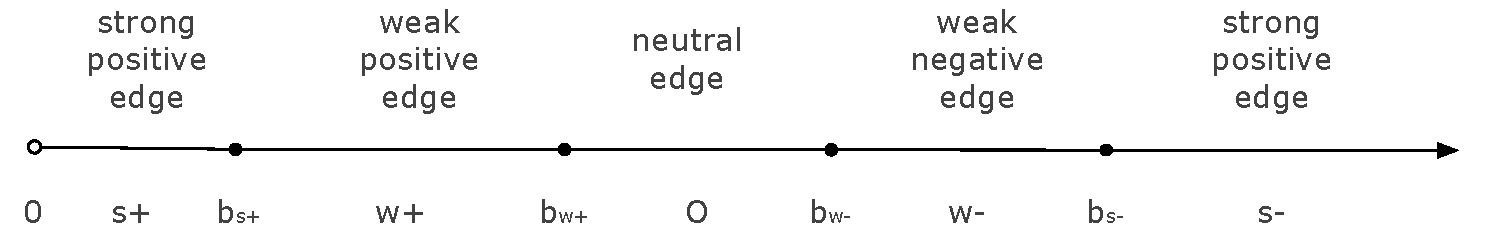
\includegraphics[height=0.55in]{mapping2.pdf}
\vspace*{-0.1in}
\caption{\label{fig:partition}Partitioning of distances:
  $[0,b_{s+}):s+$, $[b_{s+}, b_{w+}): w-$, $[b_{w+}, b_{w-}):\mbox{O}$,
$[b_{w-}, b_{s-}):w-$, and $ [b_{s-}, \infty):w+$.}

\end{figure}

In order to capture multiple relation strengths such as those
discussed in Section~\ref{sec:weak_strong}, we need multiple
thresholds. An example of the partitioning of the distance domain into
these values is given in Figure~\ref{fig:partition}. We can see that
if the following conditions are satisfied for the boundary parameters:


\begin{eqnarray*}
b_{w+}  & > & 2b_{s+} \\
b_{s-}  & > & b_{w-} + b_{s+}  \\
b_{s-}  & > & 2b_{w+} \\
b_{w-}  & > & b_{w+}+b_{s+}
\end{eqnarray*} 

\noindent the tolerance given in Table~\ref{tab:weak_strong_tolerance}
are equivalent to Definition~\ref{def:gen_tolerance}, and all triads
shown in Table~\ref{tab:imbalanced_extended} are imbalanced according
to metric triangle inequality. In other words, given any
  two distances corresponding to relation strength x and y based on
  the above thresholds, the tolerance values computed by
  Definition~\ref{def:gen_tolerance} correspond exactly to those given
  in Table~\ref{tab:weak_strong_tolerance}.

\section{Convergence Model} \label{sec:mathmodel}
Researchers have long argued that every social network has a tendency
towards a balanced state~\cite{Doreian:02}.  The next question of
interest is if an imbalance rises, in what way will a social network
change towards a new balance.  It is noted in social psychology
literature that people are reluctant to make changes in relations as
they tend to avoid the effort needed to make such changes. In a balanced
triadic relation, participants are likely to do nothing and keep their
pairwise relations as what they were. In an imbalanced triadic
relation, participants are likely to make the smallest effort possible
to regain triadic balance. We define the concept of relation cost as
the effort one needs to take to accomplish a certain relation
change. Our convergence model is established based on a unified
assumption: every social network converges in a way that requires as
little total change in relations as possible to reach a balanced
state.

With the concept of relation distance, we are able to express the
structure of a social network by drawing it in the Euclidean
space. The strength of each relation is expressed by the distance
between their locations. Notice that every layout in the Euclidean
space automatically satisfies the metric triangle inequality, and
hence corresponds to a balanced state of the network.  For an
imbalanced social network, it is not possible to draw it using its
initial relation distances.  Hence, our convergence model produces a
layout of the social network with minimum total relation cost from the
original one.

Let $G=(V,E)$ denote an arbitrary social network where $n=|V|$, and
$G^{*}=(V, E^{*})$ denote a balanced state of $G$. Let $n*n$ matrix
$X$ denote the layout of $G^{*}$, with each row vector $x_{i}$
denoting node $i$'s location in $m$-dimensional space. Note that $m$
is typically a small number such as 3 or 4 chosen for the placement of
nodes. For each pair $(i,j)$, $\psi(i,j)$ denotes its relation
distance in $G$, and $d_{i,j}(X)$ denotes distance between $i$ and $j$
in $X$, i.e., its relation distance in $G^{*}$.  Given an edge
$(i,j)\in E$, the relation cost on $(i,j)$ is given by:
\[c_{i, j}(X)=w_{\psi(i,j)}*(d_{i,j}(X)-\psi{(i,j)})^2\]
where the weight value is a function of the original distance. The
weight function can take into account the difficulty of changing a
relation. For example, it is generally easier to change a neutral
relation than a positive or a negative relation that incorporates an
initial bias. The study of optimal weights is beyond the scope of this
paper. However, we consider three main classes of weights:
\[
 w_{\psi(i,j)}= \left\{ 
  \begin{array}{l l}
    w_{+} & \quad \text{if $\psi(i,j)$ is a positive edge}\\
    w_{O} & \quad \text{if $\psi(i,j)$ is a neutral edge}\\
    w_{-} & \quad \text{if $\psi(i,j)$ is a negative edge}\\
  \end{array} \right.
\]

If $w_{O} << w_{+}$ and $w_{O} << w_{-}$, then neutral edges would
have very little influence on the already established
positive/negative relations.

\begin{definition}
Let $G=(V,E)$ be a social network where $E$ is a set of
  weighted edges. Let $G^{'}=(V,E^{'})$ be a balanced version of $G$
  obtained by changing edge strengths in $G$ with those in the layout
  matrix $X$ where $d_{i,j}(X^{'})$ based on the relation distance
  between every pair $(i,j)$.  

The cost of obtaining $G^{'}$ from $G$ is given by the difference of
the edge strengths $\sigma(X^{'})$:

\[\sigma(X^{'})= \min_{X} \sum_{i<j \leq n}w_{\psi(i,j)}*(d_{i,j}(X^{'})-\psi{(i,j)})^2\]

The convergence of $G$ is then given by a balanced version $G^{'}$ of
$G$ with the least associated total relation cost $\sigma$.
\end{definition}

\subsection{Computing Convergence}
The optimization of relation cost is in fact a Metric Multidimensional
Scaling problem (MDS) by assigning nodes a location in metric
space. The total cost function is called stress in MDS, and is often
minimized through an optimization strategy called {\it stress
  majorization (SM)} \cite {Gansner:05}. Stress majorization is an
iterative method that guarantees monotonically decreasing stress in
each iteration, and returns a locally minimum solution.  It is
recognized as a principled technique in the field of graph
drawing. The algorithm, however, requires $O(n^3)$ time and $O(n^{2})$
space. Due to its complexity, stress majorization is applicable on
graphs with limited size when missing edges are explicitly represented
as neutral ties. 

To address the issue of complexity, we also introduce an
implementation of stress majorization for sparse graphs, {\em SM/SG}
by modifying the approach in~\cite{Gansner:05}. Following Gansner's
description, we denote the d-dimensional location matrix as
$X$~\cite{Gansner:05}. Let node $i$'s location be $X_{i}$. The MDS
problem is to minimize the following stress function
\begin{equation}\label{stress}
stress(X)=\sum_{i<j} w_{ij} (||X_{i}-X_{j}|| - d_{ij})^{2}\,,
\end{equation}
where $w_{ij}$ are weights and $d_{ij}$ denote the ideal distance
between $i$ and $j$. Note that our formulation assumes that weights
remain constant throughout the convergence process. It is possible
that weights change as the underlying edge strengths change as part of
the convergence process. This alternate formulation would require
modification of our method that is beyond the scope of this current
paper.

There are many ways to minimize $stress(X)$. The iterative
majorization method at each step minimizes a simple convex function,
which guarantees a monotonically convergent solution~\cite{Leeuw:77}.
This method provides distinct advantages over localized methods like
gradient descent: it guarantees monotonic decrease of the stress
value, improves robustness against local minima and shortens
convergence time ~\cite{Gansner:05}. In application, the majorization
process involves solving the following equation iteratively:
\begin{equation}\label{recursive}
L^{w}X(t+1)=L^{X(t)}X(t),
\end{equation}
where $L^{w}$ and $L^{X(t)}$ are given by
\[
 L_{i,j}^{w}=\left\{ 
  \begin{array}{l l}
    -w_{ij} \quad & i \neq j\\
    \sum_{k \neq i}w_{ik} \quad &i=j 
  \end{array} \right. \text{,}\quad
  L_{i,j}^{X(t)}=\left\{ 
  \begin{array}{l l}
    -w_{ij}d_{ij}/||X(t)_{i}-X(t)_{j}|| \quad & i \neq j\\
    -\sum_{j \neq i}L_{i,j}^{X(t)} \quad &i=j 
  \end{array} \right. \text{ .}\]

At each iteration, $L^{w}$ is constant throughout the process, whereas
matrix $L^{X(t)}$ needs to be computed recursively. Solving
Equation~\ref{recursive} in each iteration requires the computation of
a $n \times n$ matrix, which in total requires $O(n^3)$ time and
$O(n^{2})$ space. For network of size $n> 10^{5}$, direct
implementation of stress majorization becomes impossible.

Fortunately, most social networks appear to be sparse. If we treat
all unknown edges as zero weighted, we are able to proceed. In
particular, the right side of recursive Equation \ref{recursive} can
be rewritten as
\begin{equation}\label{rightside}
(L^{X(t)}X(t))_{i}= \sum_{j \neq i} w_{ij}d_{ij} \frac {X_{i}-X_{j}}{||X_{i}-X_{j}||} .
\end{equation}
Hence, we will only need to sum up the terms corresponding to non-zero weighted edges. Let $E$ denote the number of edges of a social network, computing $L^{X(t)}X(t)$ only requires $O(E)$. 
 
For a sparse undirected network, the corresponding $L^{w}$ is sparse
and symmetric. Weighted Laplacian $L^{w}$ is known to be semi-positive
definite with a one-dimensional null space spanned by 
$1_{n}=(1,...,1)\in R^{n}$. 
We use $\bar{L^{w}}=L^{w}+ \epsilon I$ to approximate
$L^{w}$, where $\epsilon << w_{O}$ is a small positive number. Since
$\bar{L^{w}}$ becomes strictly diagonal dominant and hence positive
definite, Cholesky factorization is guaranteed to work very
efficiently.

On a single 2.8GHz processor running 64-bit Ubuntu 11.04 with 12GB of
RAM, it takes about one minute to reach convergence on our largest
data set containing 840,000 edges, requiring $O(|E|)$ space.

\begin{table}[h]
\tbl{\label{tab:algorithms} Algorithms used in this paper for solving the convergence problem.}
{
\begin{tabular}{lp{4in}}
Algorithm & Description \\ \hline
SM & Stress majorization, solution that takes into account neutral edges \\
SM/SG & Stress majorization for sparse graphs, neutral edges are given zero weight. \\
FD & Force directed graph drawing algorithm introduced in~\cite{golbeck:distrust2011} \\
PP & Path probability algorithm used in conjunction with FD in~\cite{golbeck:distrust2011}
\end{tabular}}
\end{table}


\section{Stylized Networks} \label{sec:stylized}
In this section, we use stylized networks to illustrate the notion of
convergence in small networks.  We show how positive relations cause
remaining relations to be positive and how the existence of negative
and neutral relations impact the other relations in the network. In
particular, we test the impact of positive and negative trust
relations and the transitivity of positive relations using small
networks for illustration. We will study real and large scale networks
in Section 7. For this section, we have chosen the boundary parameters
shown in Table~\ref{table:boundary_stylized}. The initial distance for
each range is set to the middle point of each range (and 1.2 for
strong negative).  The weights are chosen as follows: $w_{+}=w_{-}=1$,
$w_{O}=0.01$. We have found the converged layout of nodes in each
graph using the SM algorithm.

\begin{table}[h]
\tbl{\label{table:boundary_stylized} Boundary parameters chosen for
  the stylized networks given in Section~\ref{sec:stylized}} {
\begin{tabular}{lllll}
\multicolumn{5}{l}{Type:Bounds} \\ \hline
{\bf s+}: [0,0.1) & {\bf w+}: [0.1, 0.5) & {\bf O}: [0.5, 0.7)  & 
{\bf w-}: [0.7,1.1) & {\bf s-}: [1.1, $\infty$)
\end{tabular}}
\end{table}


\begin{figure}[th]
\centering
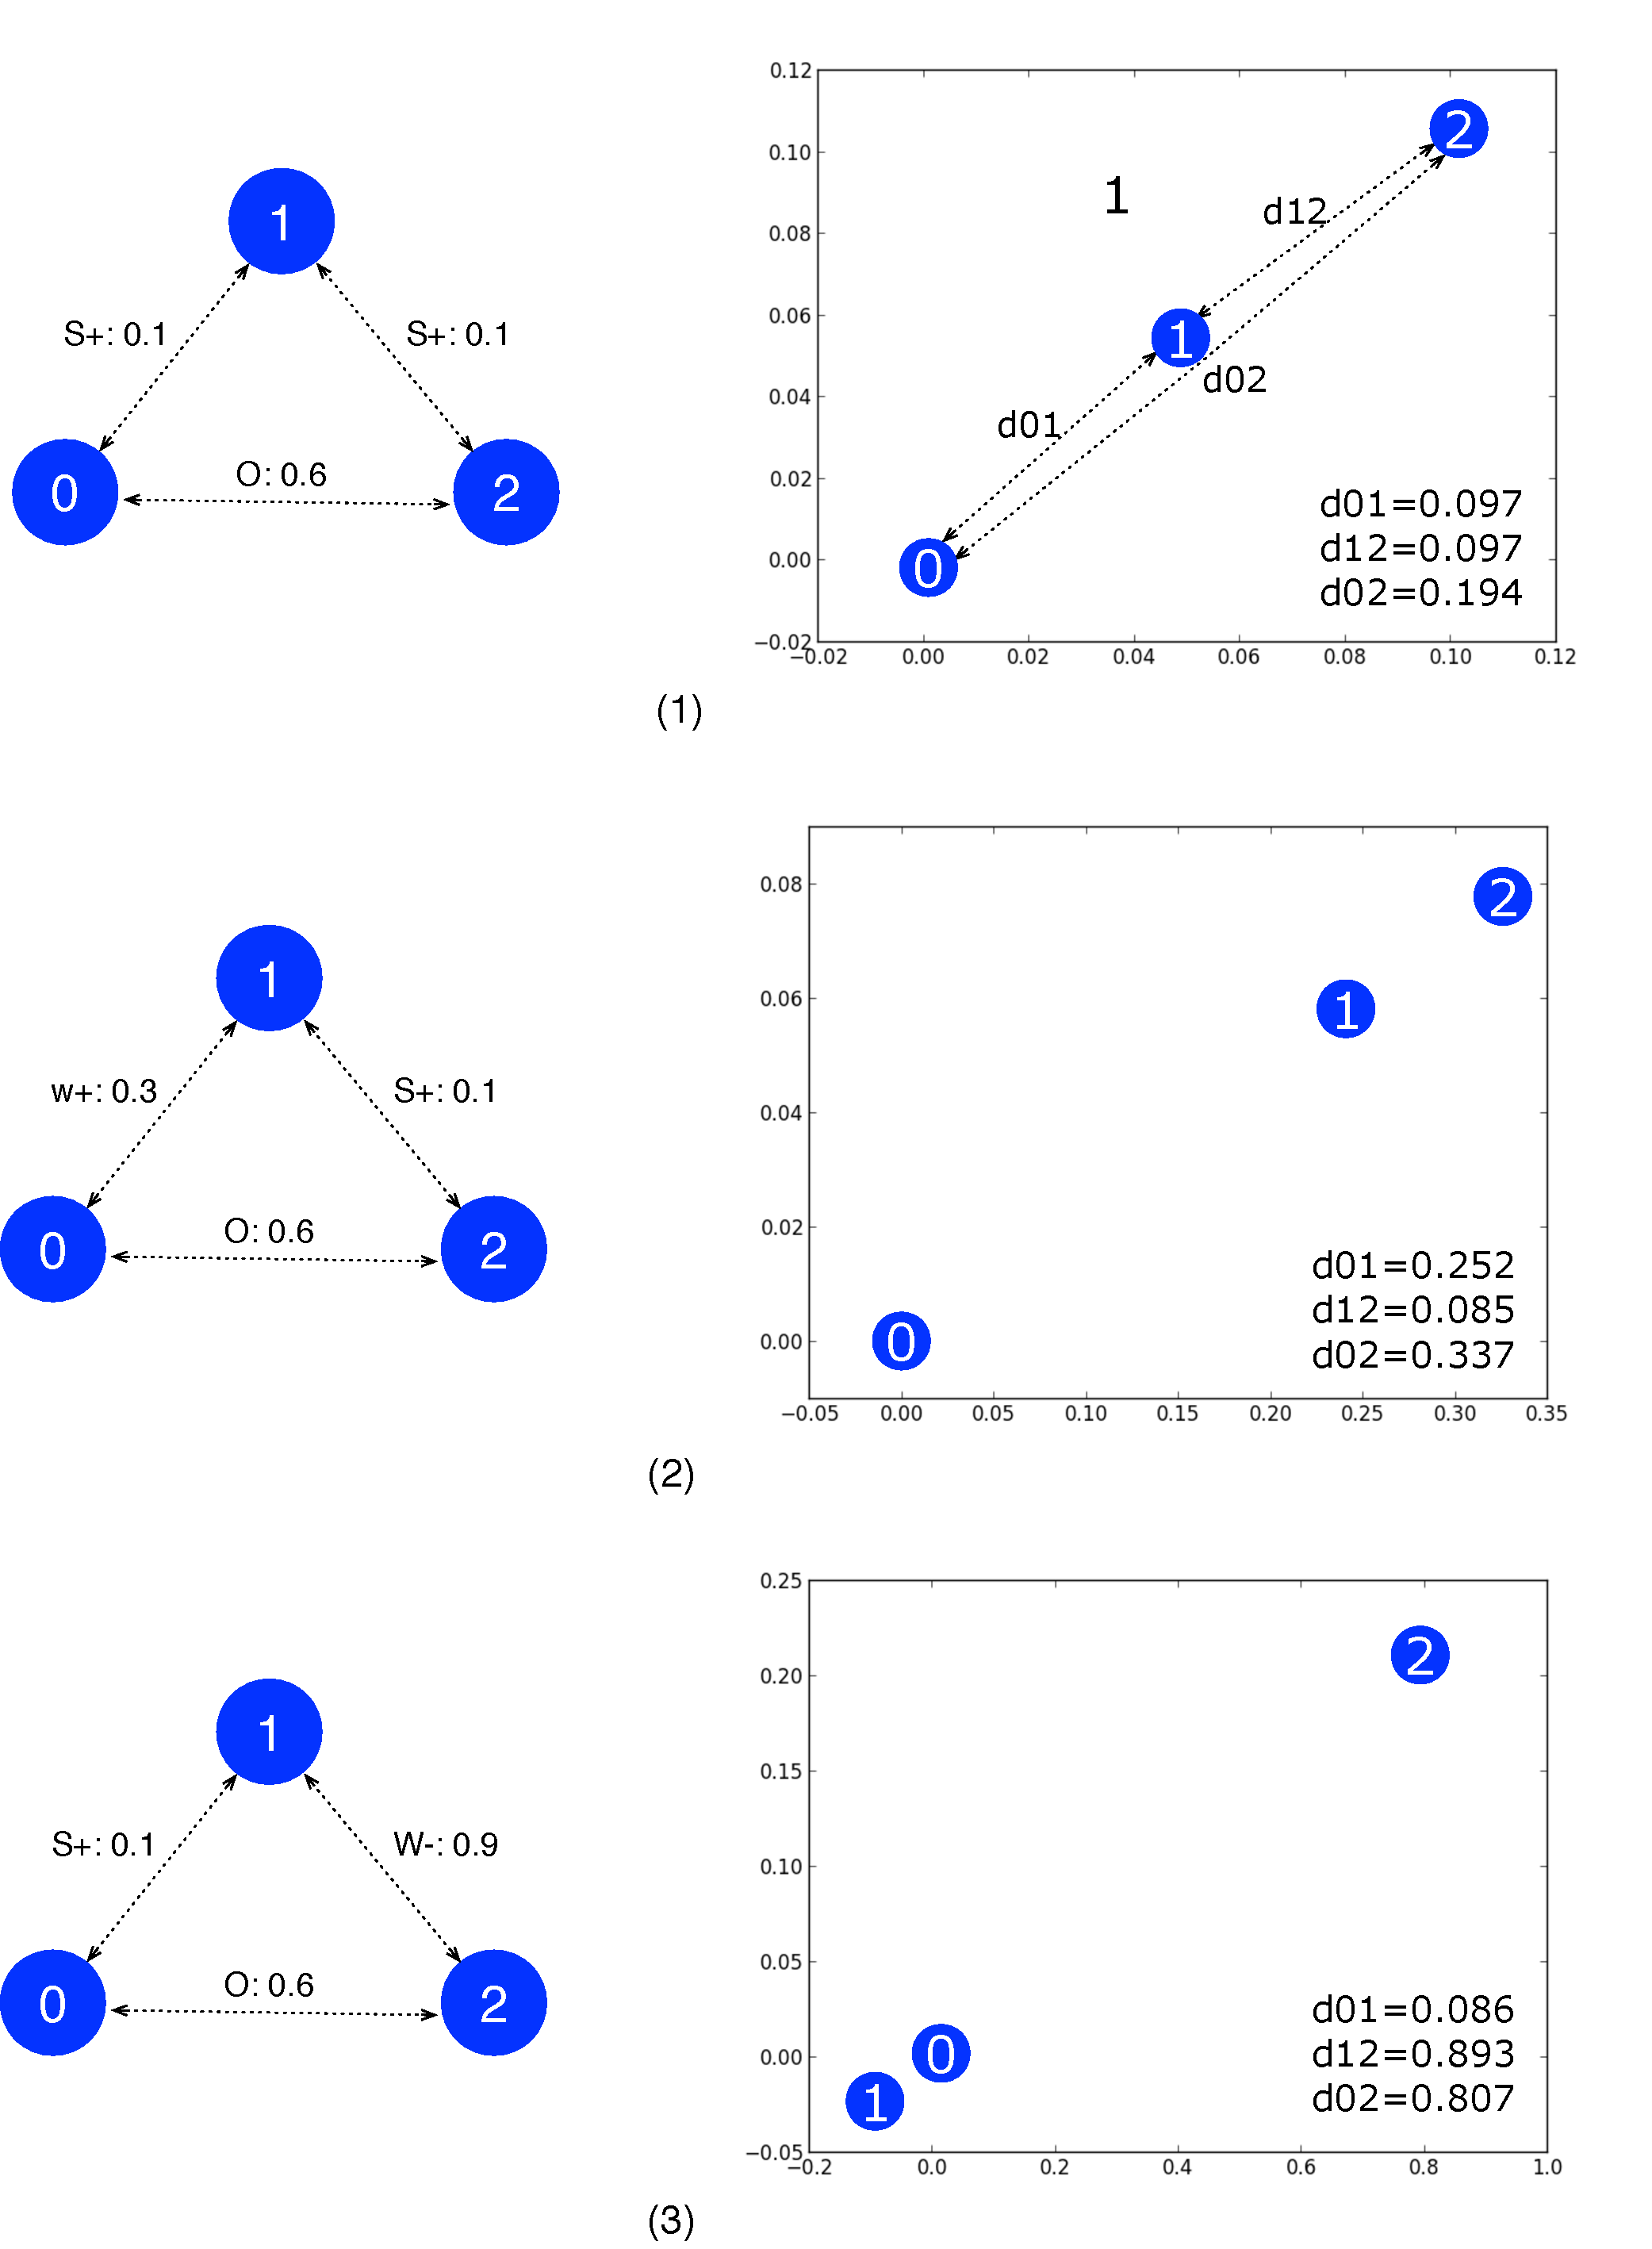
\includegraphics[width=3in]{stylized1.pdf}
\caption{\label{fig:style1} Convergence of networks containing neutral edges.}
\end{figure}

\subsection{Convergence of networks with neutral edges.}
First, we look at convergence for different networks containing
neutral edges. We consider three networks in Figure~\ref{fig:style1}
containing a single neutral edge between nodes 0 and 2. The initial
values for relation strengths is given in the graph on the left. The
converged location for the nodes is shown on the right. The first
graph contains two strong positive edges and a neutral edge. After
convergence, the neutral edge has changed to a weak positive node.  As
a result, the two strong positive edges were above the threshold that
requires the remaining edge to be a positive relation. These two edges
remain strong positive after convergence. This graph illustrates
principle 1.

Next, we look at graph 2 in Figure~\ref{fig:style1} which contains a
strong positive and a weak positive edge in addition to the neutral
one. As expected, the neutral edge becomes a weak positive edge after
convergence. However, as expected from principle 1, since the pull is
lower in graph 2 than in graph 1, the strength of edge (0,2) is also
weaker in graph 2 than in graph 1 after convergence.

Finally, we look at graph 3 in Figure~\ref{fig:style1} which contains
a strong positive and a weak negative edge. Based on principle 2, due
to the large difference in strengths, we expect that the relation
between 0 and 2 cannot remain neutral and it will become negative. In
fact, after convergence, edge (0,1) remains strong positive, edge
(1,2) remains weak negative, and the edge (0,2) becomes weak negative.


\begin{figure}[th]
\centering
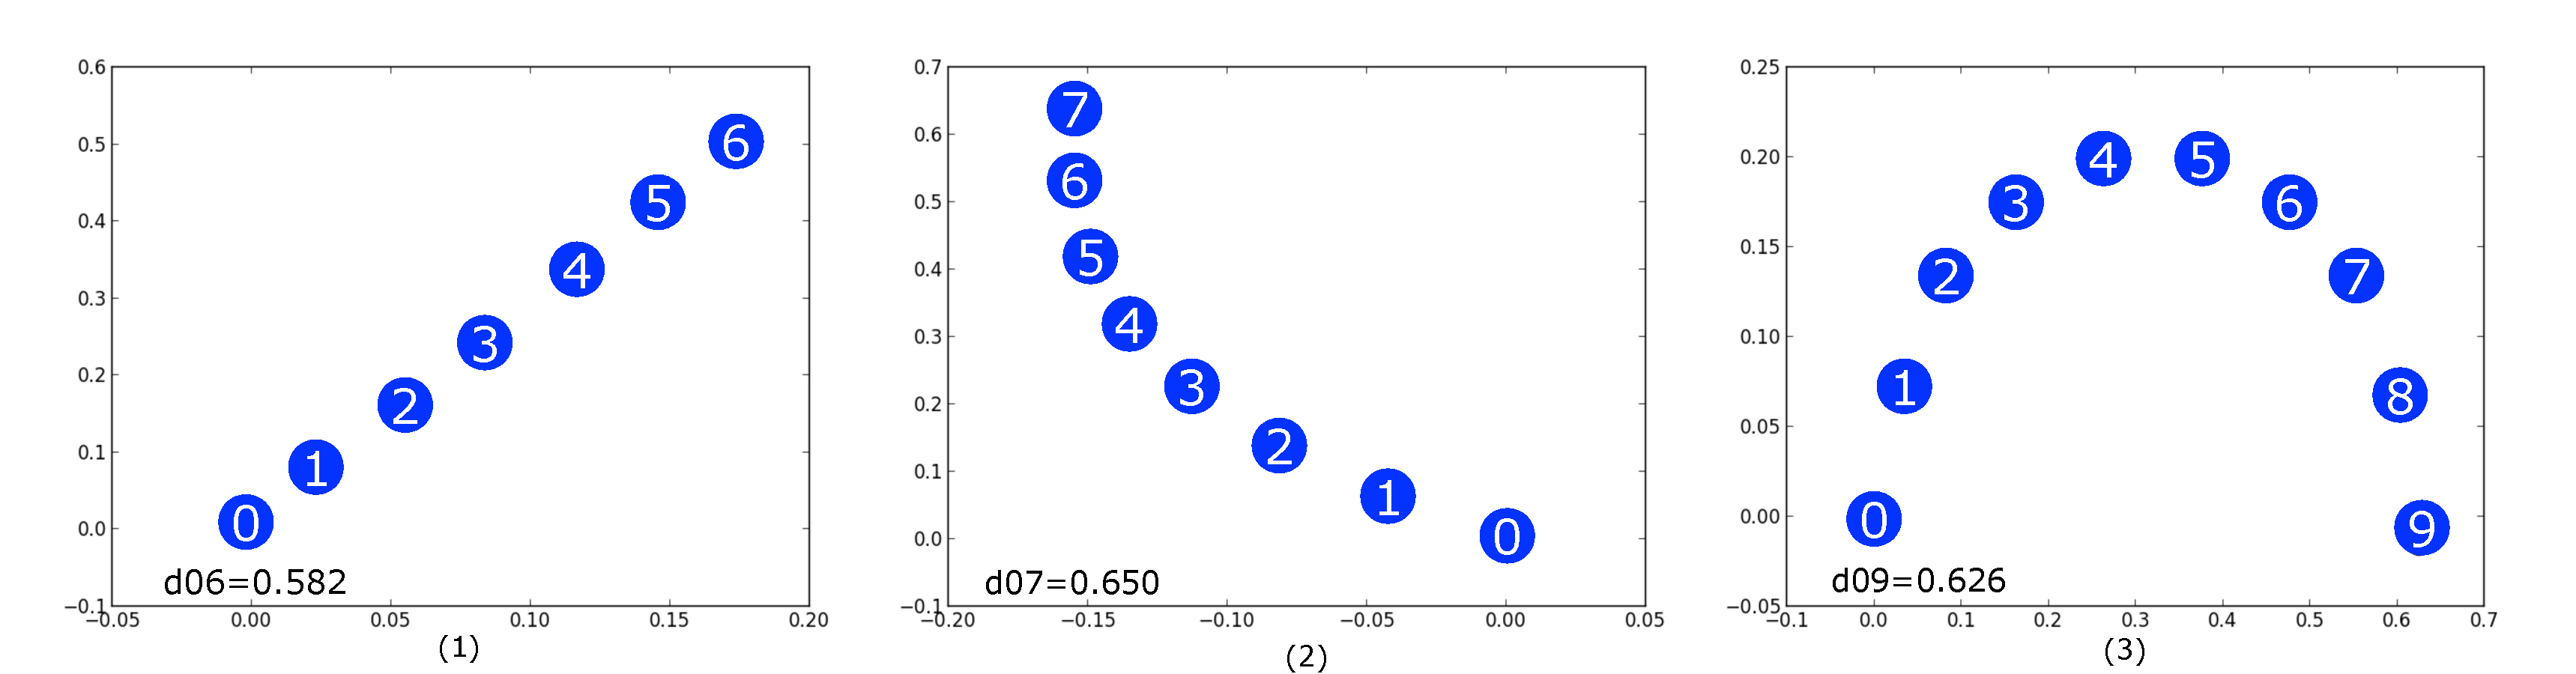
\includegraphics[width=5.5in]{stylized2.pdf}
\caption{\label{fig:style2} Transitivity of positive edges.}
\end{figure}


\subsection{Transitivity}
Next, we consider transitivity of positive edges. This is an often
assumed property of trust relationships in networks. For example, if
Alice trusts Bob and Bob trusts Charlie, it is likely that Alice
trusts Charlie. If Charlie trusts Dana, then it is also likely that
Alice will trust Dana. But, as the chain gets longer, the effect is
expected to get weaker. Furthermore, the existence of positive chains
does not put any stress towards negative values on the such
relationships and principle 2 is never applied. Hence, after
convergence, the existing edges should remain positive and neutral
edges should become positive or stay neutral.  To test whether this
property holds in our model, we consider graphs of $n$ nodes arrange
on a single line, e.g. (0,1), (1,2), (2,3), etc. Each edge is a strong
positive. Graphs 1,2 and 3 in Figure~\ref{fig:style2} show
transitivity of 7,8 and 10 nodes. Note that these graphs are very
sparse, containing only $n-1$ edges. The converged relations display a
number of desirable properties. First, pairwise distances of existing
edges remain strong positive. Secondly, the longer the path between
two nodes in the graph is, the larger is the Euclidian distance
between them. This follows the often hypothesized property of
attenuation of trust along longer paths. We also note that the largest
distance, between nodes (0,6) in graph 1 (as well as (0,7) and (0,9)
in graphs 2 and 3) remain a neutral edge. In fact, this is achieved by
curving the underlying placement of nodes in graph 3.


\begin{figure}[th]
\centering
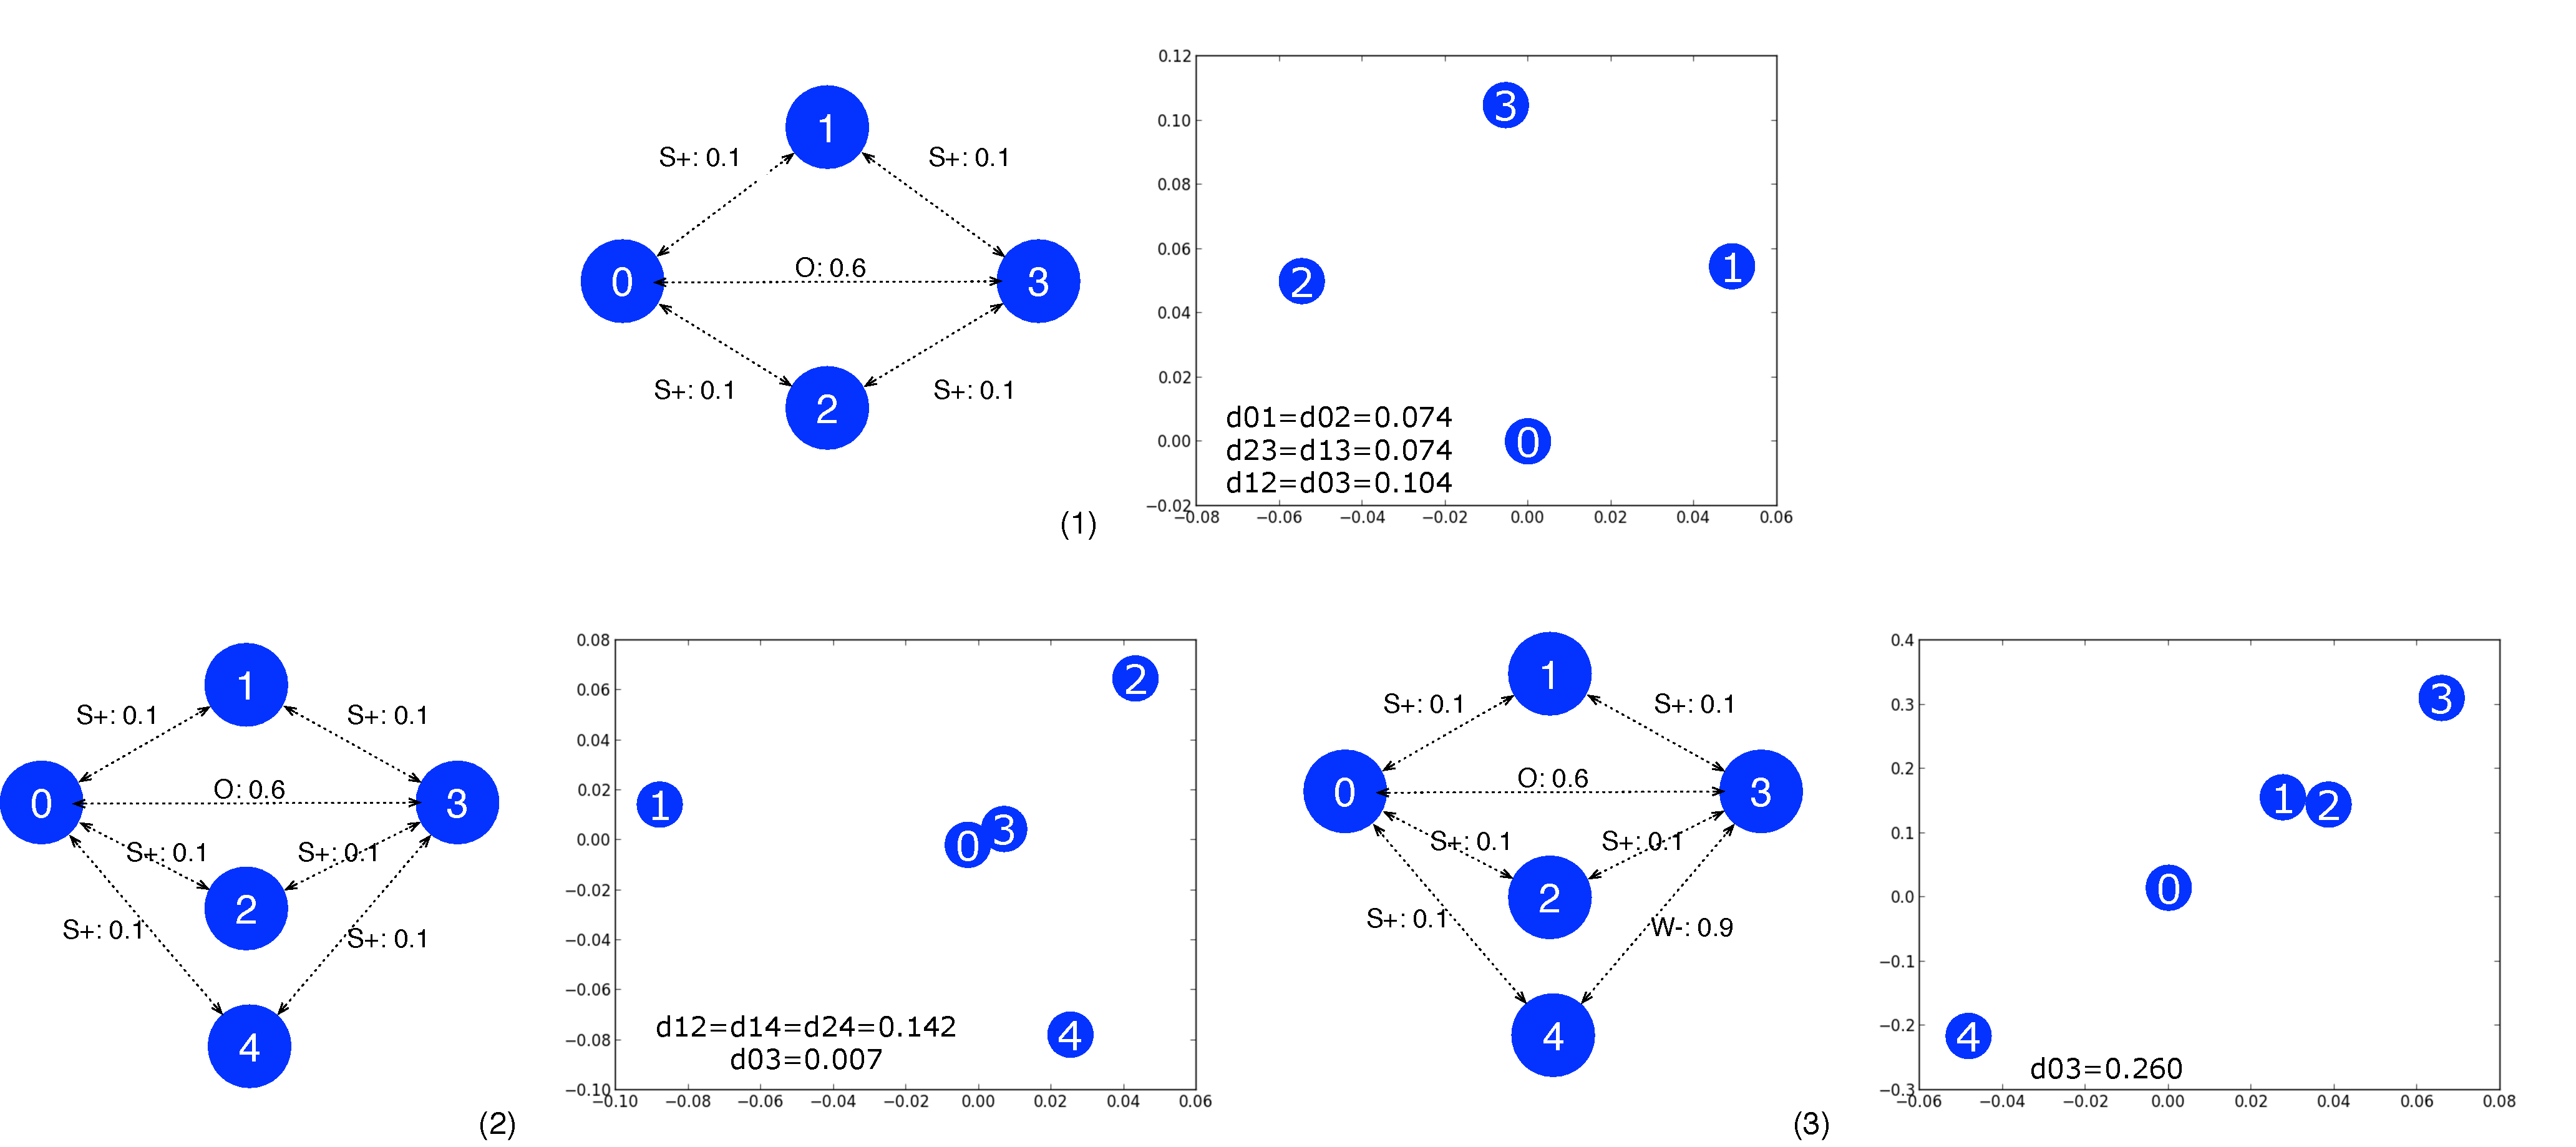
\includegraphics[width=5.5in]{stylized3.pdf}
\caption{\label{fig:style3} Impact of increasing connectivity in convergence.}
\end{figure}

\subsection{Aggregation}
Finally, we study the aggregate effect of having multiple paths
between two nodes. We are first given graph 1 in
Figure~\ref{fig:style3}. Given two triangles containing strong
positive edges, the originally neutral edge (0,3) becomes weak
positive after convergence. In fact, the strength of the edge is
0.104, an almost strong positive edge.

Next, we consider adding other paths between nodes (0,3) and
investigate the effect. In graph 2, we add another triangle with two
strong positive edges. The effect of this is to cause (0,3) to come
even closer and become a strong positive edge. In other words, as more
positive paths between the two nodes are added, the more positive they
become.

In graph 3 of Figure~\ref{fig:style3}, we add a path containing a
strong positive and a weak negative edge. Due to the difference in the
strengths of these edges, we expect that they would exert a negative
influence on (0,3). In the converged network, the edge (0,3) is weak
positive with distance 0.26. In fact, the strength of edge (0,3) is
weaker than in both graphs 1 and 2. This is an expected result as there
is no negative influence in any of the other networks.

This indicates that adding a common friend between two people will
grant a better chance to them to become friends. However, adding a
conflicted common neighbor between two people will deteriorate their
relationship.

Overall, our results in stylized networks illustrate that the
convergence formulation results in intuitive results. 

\begin{algorithm}\label{alg}
 \KwData{${\cal A}$, $M, k, deg, G$}
 \KwResult{$Pt, Nt$}
 Get $G'=$ generate-subgraph$(M, k, deg, G)$\;
 Partition $G'$ into 10 groups of test and training samples\;
 Create two empty sets $Pt$, $Nt$\;
 \For{each of the groups}{
 run algorithm ${\cal A}$ on the training sample and get the layout\;
 \For{each edge e in the testing sample}{
 compute its distance in the layout\;
 \eIf{e is a positive edge}{
   add its distance to $Pt$\;
   }{
   add its distance to $Nt$\;
  }
 }
 }
 \caption{Edge Sign Prediction Methodology}
\end{algorithm}



\section{Experimental Setup} \label{sec:setup}
In the next section, we study the various properties of our framework,
in particular its application to the {\it edge sign prediction
  problem} for various real networks.  The {\it edge sign prediction
  problem} is defined as follows. Suppose we are given a social
network with signs, but a small fraction of the edge signs are
``hidden''. How can we predict these signs with the information
provided by the rest of network?  The convergence model is able to
predict these ``hidden'' signs. Let's denote the original social
network with all signed edges as $G$, the network consisting of hidden
edges as $G_{h}$, and the network consisting of the remaining edges as
$G_{r}$. The edges (relations) between each pair of nodes is measured
by $\{+,\,-,\,O\}$. We run the convergence model on $G_{r}$, and
denote the network after convergence as $G_{r}^{'}$. We expect that
the signs of the hidden edges in $G_{r}^{'}$ largely agree with the
true signs.

By the assumption that every social network has a tendency towards
balance, it can be inferred that $G$ is largely balanced at any
moment. Hence, the majority of $G_{r}$ is balanced. The only
exceptions are the components with hidden edges, which are of sign $O$
in $G_{r}$. By the principle of total relation cost minimization, the
changes mostly occur on the $O$-sign hidden edges during the
convergence. We expect the hidden edges in $G_h$ to have their true
signs in $G_{r}^{'}$ if $G$ is largely balanced. Hence, we test the
performance of an algorithm by first randomly sampling 90\% of the
edges of a given graph as the training graph (e.g. $G_{r}$) and set
aside the 10\% as the test data (e.g. $G_h$). We then find the
distance between nodes in $G_h$ with respect to the converged version
$G_{r}^{'}$ of $G_r$. We use the algorithms given in
Table~\ref{tab:algorithms} for finding a converged graph. We repeat
each experiment 10 times.

The distances of testing edges are computed by the layout of the
training data. Given a distance threshold, the sign of each edge is
predicted as positive if and only if its distance is smaller than the
threshold. In the previous work, such threshold is computed from the
(distance,sign) pairs of the training samples using standard machine
learning
techniques~\cite{golbeck:distrust2011}\cite{Leskovec:2010}. In this
paper, however, we do not concentrate on the learning process. The
issue of interest is how well the convergence model performs in
separating hidden positive edges from negative ones in terms of
distance. Instead of making predictions based on a particular
threshold, we draw ROC curves for evaluation which capture the
performance of sign prediction for both positive and negative edges
across all thresholds and compute the false and true positive rates
based on the computed $Pt$ ($Nt$) values returned by the
Algorithm~\ref{alg}. The ROC curves are drawn upon the $Pt$ ($Nt$)
values from the accumulation of all testing samples.

In the implementation of SM and SM/SG, the weight of each type of edge
satisfies:
\[ w_{O}<<w_{+}<\frac{w_{-}}{2}. \] 
The first inequality has been argued in the previous section. The
second one is chosen empirically, indicating that a negative edge has
larger influence than a positive one.  We repeat the experiments on
various weights and original distance configurations under the above
two constraints, the prediction performance turns to be very
consistent. We present sensitivity results in the next section.

The partitioning of the distance domain satisfies
\[ b_{+} < \frac{b_{O}}{2} < \frac{b_{-}}{2} \]
for a positive, neutral and negative edge, conforming to our
theory. Hence, the initial values for distances of a positive edge $d_{+}$, a neutral edge $d_{O}$ and a 
negative edge $d_{-}$ should at least satisfy $b_{+} < \frac{d_{O}}{2} < \frac{d_{-}}{2}$.
One of the recommended parameter configurations is given as
the following.
\begin{table}[htp]
\tbl{\label{tab:PP}The recommended parameter configuration.}{
\begin{tabular}{lllllll}
 Parameter & $w_{+}$ & $w_{O}$ & $w_{-}$ & $d_{+}$ & $d_{O}$ & $d_{-}$ \\  \hline
Configuration &1.0 & 0.01 & 3.0 & 0.1 & 0.6 & 1.1  \\ 
\end{tabular}}
\end{table}

Note that SM/SG does not consider neutral edges and as a result it
implicitly assumes that $w_{O}=0$.  We use the same setting for all
the networks and do not employ any other adjustable parameters unless
explicitly specified. In Section~\ref{sec:tiestrength}, we employ a
version of our algorithm that considers tie strength as well. We give
the parameters used for this version in the relevant section.


\subsection{Datasets studied}
We use the same three datasets used
in~\cite{golbeck:distrust2011} and~\cite{Leskovec:2010} to conduct our
experiments, all provided by the Stanford Large Network Dataset
Collection. 

\begin{enumerate}
\item {\em Epinions} is a product review website where users give
  reviews and ratings on product articles. Users can choose to trust
  or distrust others. The network contains more than 100,000 users and
  over 700,000 trust/distrust edges. There are also 13,668,320 ratings
  for 1,559,803 articles. We use the ratings only for external
  validation. 

\item {\em Wikipedia} elections collects the votes by Wikipedia users in
  elections for promoting candidates as administrators. Each user can
  give a supporting (positive) or opposing (negative) vote on the
  promotion of another. The dataset has about 7,000 users and around
  100,000 votes (edges) for 2,794 elections.

\item {\em Slashdot} is a technology news website where users rate
  each other as friends or foes. The dataset released in February 2009
  contains over 77,000 users and over 900,000 friend/foe edges. 
\end{enumerate}

Overall, we note that the trust ratings in Epinions is more of a vote
of competence, whereas in Slashdot, it is more of a rating of
trustworthiness (constructs like reliability, friendliness, etc.). The
ratings in Wikipedia fall somewhere in between the two, incorporating
both aspects of competence and trustworthiness. Wikipedia
administrators are expected to be both competent in their job, but
also not subvert the power of their position. We expect 
structural balance to be more applicable to trust ratings of
trustworthiness. While the affective aspect of trust relations based
on trustworthiness impact the competence judgments, there is no
parallel notion of stress in trust relations based on competence. As a
result, we expect our theory to be most applicable to Slashdot.

There is also difference in the fraction of positive votes to negative
votes in the data sets. In Epinions, there is a negative vote for
every 5.8 positive vote. This number is 3.63 for Wikipedia and 3.43
for Slashdot. As a result, capturing the meaning of distrust relations
becomes even more important for Wikipedia and Slashdot.

\subsection{Graphs used in the experiments}
Using these networks, we construct different graphs to test the
different hypotheses made in this paper. Even though the edges in the
underlying networks are directed, we construct several undirected
graphs out of these networks. In this process, we consider four types
of edges:

\begin{enumerate}
\item {\em Bi-directional edges} are reciprocal signed edges. For each
  edge $(A,B)$, the network contains both directed edges $(A,B)$ and
  $(B,A)$ with the same sign. 

\item {\em Single directional edges} are non-reciprocal edges. For
  each edge $(A,B)$, there is a directed edge $(A,B)$, but no edge
  $(B,A)$. 

\item {\em Known neutral edges} are edges $(A,B)$ such that either
  there are the directed edges $(A,B)$ and $(B,A)$ with conflicting
  signs, or one of $(A,B)$ or $(B,A)$ is explicitly a neutral
  edge. Neutral edges only exist in Wikipedia where the votes can be
  positive, negative or neutral.

\item {\em Unknown edges} are any pair of nodes with no edge in
  between.
\end{enumerate}

Given these edges, we construct the graphs given in
Table~\ref{tab:graphtypes}. They are roughly ordered from general to
specific. Notice that for each pair of reciprocal signed edges, we add
a single undirected edge in the constructed graph to avoid
duplications.


\begin{table}[htbp!]
\tbl{\label{tab:graphtypes} The different graphs constructed from
  the given networks in our experiments.}{
\begin{tabular}{p{0.4in}p{2.0in}p{2.0in}}
Graph &  Positive/Negative Edges & Neutral Edges   \\ \hline

G$^*$ & Single and bi-directional edges are signed as positive or
negative, no tie strength. & Unknown and known neutral edges. \\ \hline

G & Same as G$^*$ & Only the known neutral edges.  \\ \hline

G$^\#$ & Same as G$^*$ & The known neutral edges and unknown edges
between any pair of nodes that are connected by a path of length
2. \\ \hline

G-bi & Only bi-directional edges are signed as positive or negative. &
Only the known neutral edges. \\ \hline 

G-di & Bi-directional edges are considered strong ties, single
directional edges are considered weak ties. & Only the known neutral
edges. \\ \hline
\end{tabular}}
\end{table}

The sizes of the various graphs for each network are given in
Table~\ref{tab:graphsize}. We note that for Wikipedia, there are only
around 1/33 edges bi-directed. If a node $A$ has voted on $B$, then
$A$ is an admin. Hence, even if $B$ becomes an administrator, it is
extremely rare for $B$ to vote on $A$ later on. As a result, the
graphs in G-bi in Wikipedia are too small for representative
results. In comparison, around $1/6$ of the edges in Epinions are
bi-directed and around $1/10$ of the edges in Slashdot are
bi-directed. For these graphs, it is possible for edges to
independently review each other in either direction.

\begin{table}[htp]
\tbl{\label{tab:graphsize} The size of the different graphs (in terms
  of number of edges) constructed from the given networks in our
  experiments. Note: for G$^*$ we only provide the number of known
  edges in sampled graph sizes.}{
\begin{tabular}{llll}
Graph & Epinions &  Wikipedia & Slashdot  \\ \hline
G$^*$ &180,000  &160,000 &65,000  \\ 
G & 841,000 & 100,000 & 549,000 \\
G$^\#$ &45,400,000  &1,600,000 &14,200,000 \\ 
G-bi &128,000   &3,000 &48,000  \\ 
G-di &704,000   &105,000 &495,000  \\ 
\end{tabular}}
\end{table}

The graphs considered in this paper, in particular G$^*$, are dense
(similar in size to G$^\#$). After we add the unknown neutral edges,
G$^*$ becomes a complete graph.  It is practically infeasible for SM
to run on the entire dataset for any version of the graphs. This is
due to large number of neutral edges that must be explicitly
represented to run SM.  In practice, we will evaluate the performance
of SM on small sub-networks of G$^*$ computed by sampling only. To
accomplish this, we generate random samples of our datasets using the
snowball sampling method in which a small number $k$ of seeds with
degree greater than a given threshold $deg$ are selected at random,
then all nodes that are adjacent to the seed node are selected
iteratively until the desired network size is reached.  In our
practice, the size of the resulting graph is in the range 3,000-5,000
nodes, $k$ is chosen from 2-10 randomly and $deg$ is chosen from 7-20
randomly. For each dataset, we generate 10 sub-networks and perform
10-fold cross validation. The number of known edges in a sub-network
of Epinions is around 180,000, for Slashdot 65,000 and for Wikipedia
160,000.

In our first set of results, we compare the performance of SM to our
baseline algorithm, FD using sampled graphs as well as performance of
SM/SG on the full graph.


\begin{figure*}[thbp!]
\tbl{\label{fig:ROC} The ROC curves are drawn upon distances of hidden
  edges for samples of G$^*$ for Epinions, Slashdot and Wikipedia
  datasets. Comparison between SM in Figures 1.a, 1.b, 1.c, and SM/SG
  in Figures 2.a, 2.b, 2.c. Area under the curve of (SM, SM/SG, FD) for
  Epinions: ({0.954}, {\bf 0.956}, 0.946), Wikipedia: ({\bf 0.927},
  0.926, 0.899), and Slashdot: ({\bf 0.954}, 0.954, 0.907).}{
\begin{tabular}{ccc}
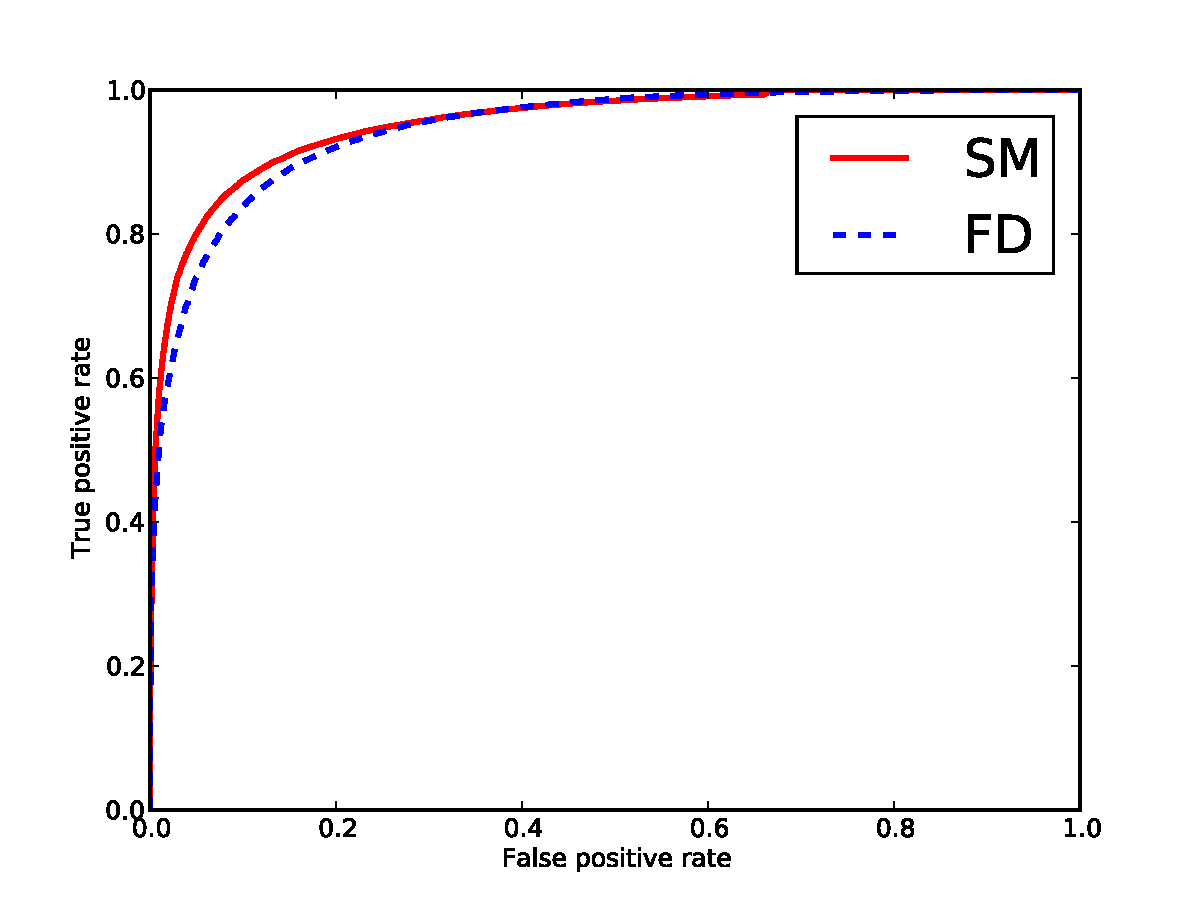
\includegraphics[width=1.7in]{SM_Gstar_ep.pdf} 
&
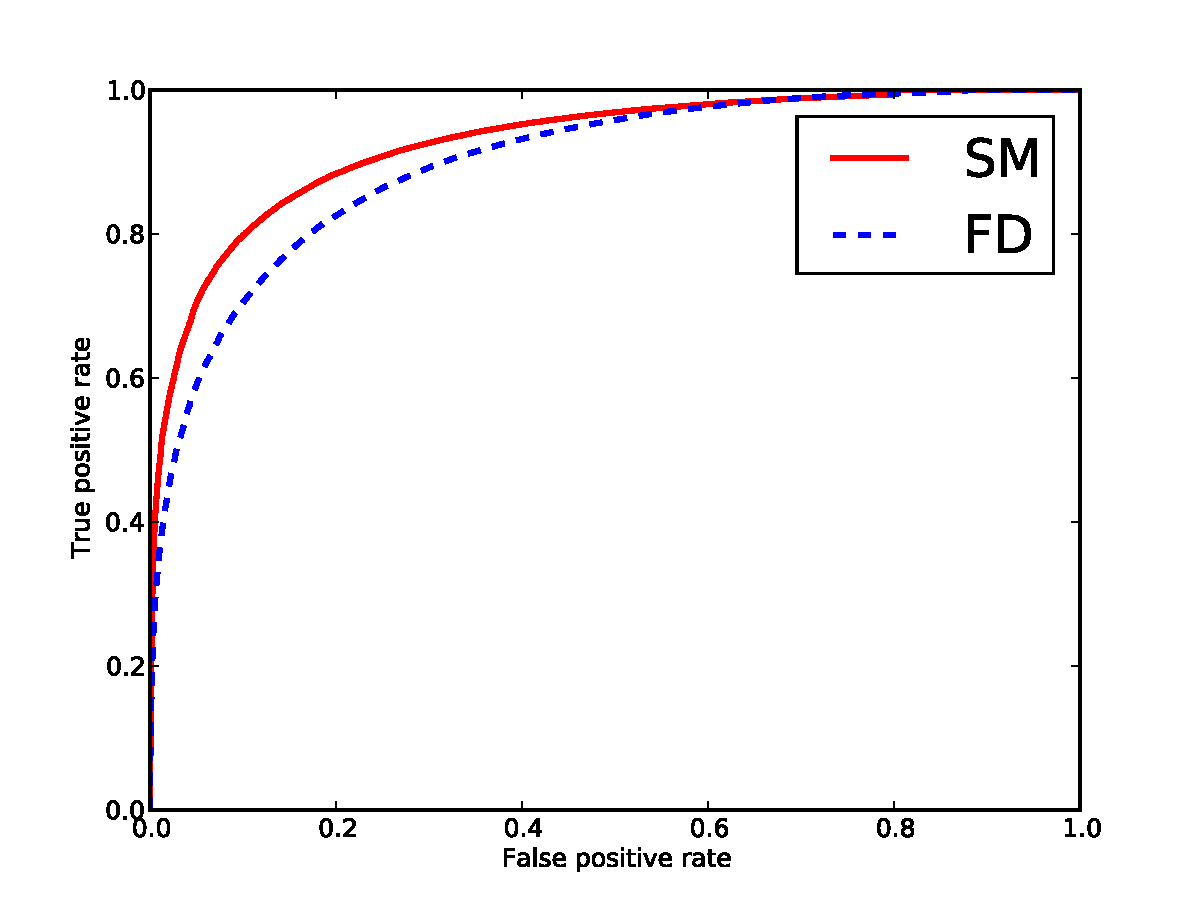
\includegraphics[width=1.7in]{SM_Gstar_wiki.pdf} 
&
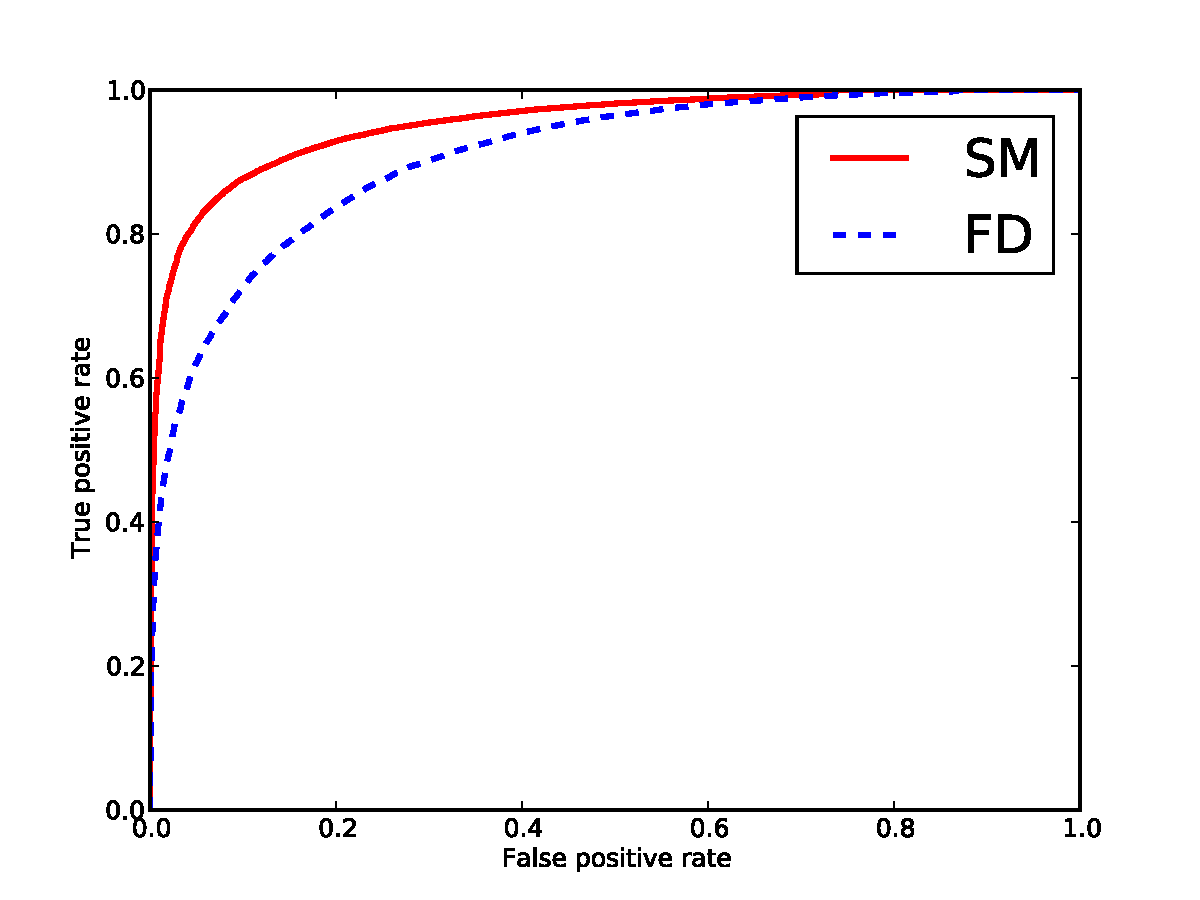
\includegraphics[width=1.7in]{SM_Gstar_slash.pdf} \\
(1.a) Epinions & (1.b) Wikipedia & (1.c) Slashdot \\
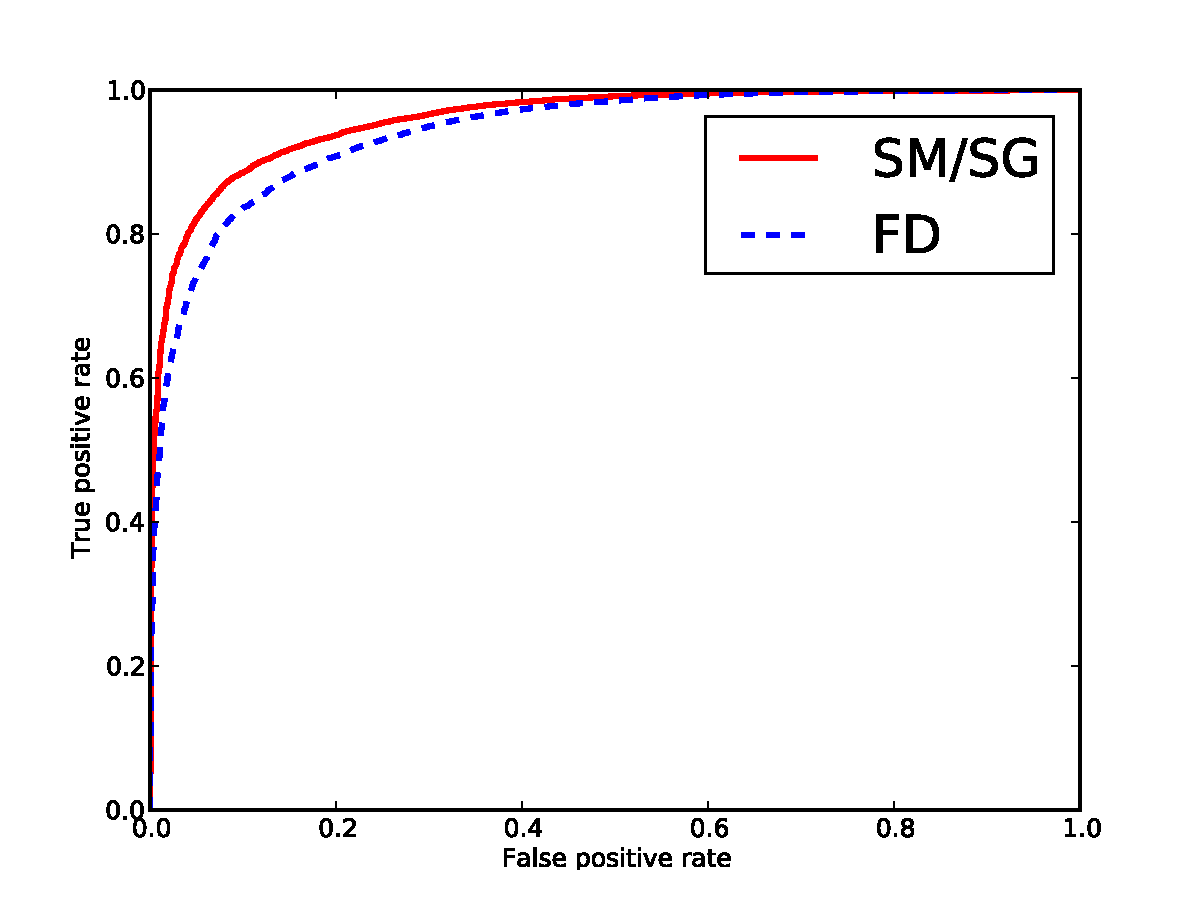
\includegraphics[width=1.7in]{SMSG_Gstar_ep.pdf} 
&
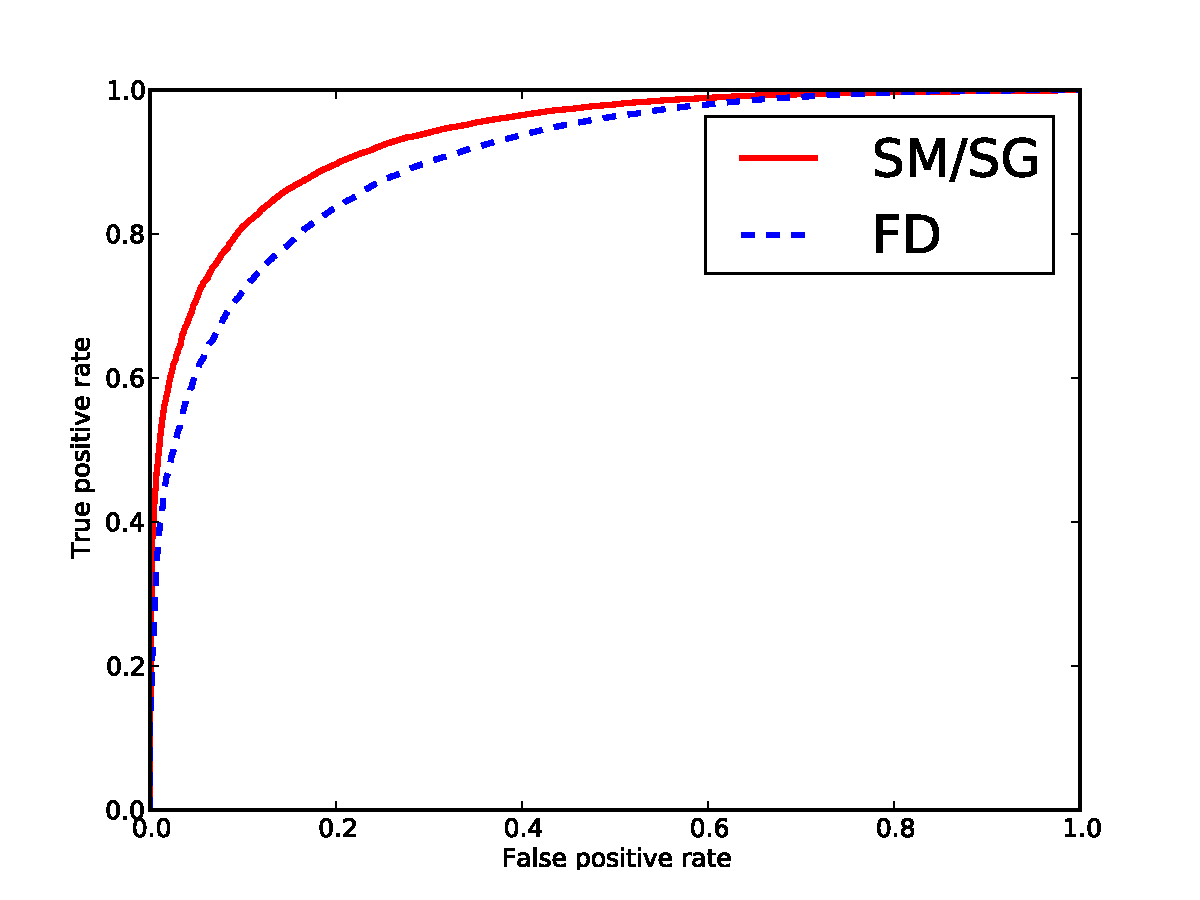
\includegraphics[width=1.7in]{SMSG_Gstar_wiki.pdf} 
&
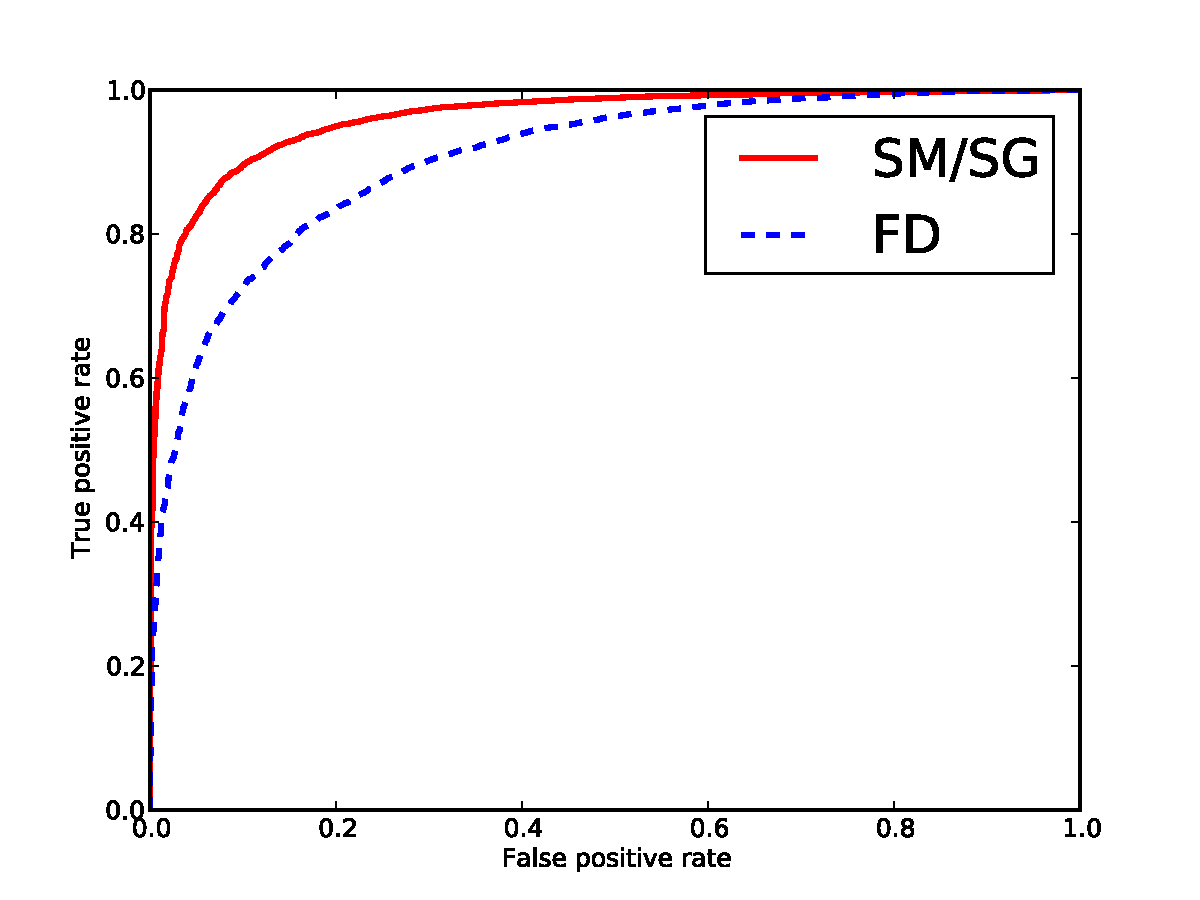
\includegraphics[width=1.7in]{SMSG_Gstar_slash.pdf} \\
(2.a) Epinions & (2.b) Wikipedia & (2.c) Slashdot
\end{tabular}}
\end{figure*}


\section{Experimental Results} \label{sec:results}
In this section, we focus on the {\it edge sign prediction problem}
unless otherwise stated. We compare our algorithm with the force
directed algorithm (FD) in~\cite{golbeck:distrust2011} as this
algorithm's performance has been shown by the authors to be the state
of the art for measuring trust and distrust. Note
that we have tuned our implementation of FD to provide similar
performance reported in this work. Even though this work combines two
algorithms, FD and PP, in our comparison experiments, we find that FD
alone gives equally good prediction performance on all three datasets
as the combination. The comparison is shown in Table~\ref{tab:PP}. As
a result, we will only compare our method with FD in the following
discussion. Note that all the results reported in this section are
highly significant. The variation in the values reported (with the
exception of tests involving the last 10\% of the edges) have very
small variation, below 0.001 in most cases. For this reason, we will
not put error bars on our graphs.

\begin{table}[htp]
\tbl{\label{tab:PP} The prediction performance by FD and FD$\&$PP on
  G$^{*}$, in terms of prediction accuracy on positive and
  negative edges, on all three datasets. The probability parameter $p$
  is set to $0.05$ as it is in~\cite{golbeck:distrust2011}.}{
\begin{tabular}{lllllll}
 & \multicolumn{2}{c}{Epinions} &  \multicolumn{2}{c}{Slashdot} &  \multicolumn{2}{c}{Wikipedia}  \\
Method & Positive & Negative & Positive & Negative & Positive & Negative \\  \hline
FD &90\% & 87\% &83\% & 80\% &82\% & 79\%  \\ 
FD\&PP &88\% & 88\% &82\% & 80\% &82\% & 80\%  \\ 
\end{tabular}}
\end{table}

In the remainder of this section, we provide experimental
  results to illustrate the following points.
\begin{itemize}
\item First, we show that our algorithm outperforms FD on complete
  graphs, considering any missing edges as neutral. Due to the large
  size of such graphs, we only use samples
  (Section~\ref{sec:gstar-results}).
\item Next, we use sampled graphs again to show that performance does
  not degrade much when we disregard the neutral edges that are added
  when an edge is missing (Section~\ref{sec:neutral_edges}). In
  essence, neutral edges provide information but also introduce
  noise. Given that our algorithm still outperforms FD in this
  setting, for the remainder of the tests, we disregard such neutral
  edges. This allows us to run experiments using the full datasets
  for the following cases.
\item We show that our method is able to capture the notion of
  convergence, the fact that one's trust for others may change over
  time due to pressure from one's social circle. We use Epinions with
  two proxies for trust, explicit trust ratings and implicit trust
  ratings in the form of ratings of reviews.  We compute convergence
  using only the explicit trust ratings and compare this to the implicit
  ratings. For all edges, the average review rating value seems to
  increase over time, but less so for negative edges. However, it
  increases significantly for negative edges flipped by our algorithms
  after convergence (Section~\ref{sec:external}).
\item We investigate whether selecting neutral edges better can lead
  to improved performance by considering the notion of transitivity:
  friends of friends are likely to know each other. We introduce these
  as neutral edges. Overall, the performance of both algorithms suffer
  in this case due to the additional noise incorporated in this
  setting: while we added some likely edges, we also added many
  nonexistent edges. Furthermore, this is worse in Wikipedia in which
  edges are more likely to be based on competence and have weaker
  overall strength (Section~\ref{sec:indirect-neutral}).
\item We show that the performance of our algorithm degrades
  gracefully as we remove more and more of the edges. Only after
  removal of 90\% of the edges, we see a significant performance
  drop. The existence of negative edges and the structural balance
  formulation results in very robust results
  (Section~\ref{sec:coverage}).
\item We study whether our algorithm can help predict the trust links
  for newcomers to the network. The problem is hard as these nodes have very few links to the other nodes. While our algorithm outperforms FD, the
  prediction rate is relatively poor in Wikipedia and slightly better
  in Epinions. (Section~\ref{sec:results-time}).
\item We then consider whether we can improve the performance of the
  algorithm by considering weak and strong edges. In this case, strong
  edges are those with the same sign on both directions. Edges with a
  single direction are weak, and edges with mixed signs are considered
  neutral. We have already shown that these edges were meaningful in
  Epinions (Section~\ref{sec:external}) as the average ratings for the
  reviews for these correlate with the trust values. Our prediction
  for strong edges is much higher than FD in this case, and the
  prediction for weak edges still remains higher than FD. In addition,
  this effect becomes more pronounced in Slashdot which relies on
  friend/foe characterization than in Epinions which is a competence
  based trust rating (Section~\ref{sec:tiestrength}).
\item We show that our algorithm is not sensitive to choice of
  parameters (Section~\ref{sec:sensitivity}).
\item Finally, we show that unknown edges in our method are
  distributed evenly across the distance range, making it easier for
  edge prediction methods to be built on top of our algorithm. We use
  the sampled graphs for this
  result. (Section~\ref{sec:link-prediction}).
\end{itemize} 

\subsection{Performance of SM on G$^*$.} \label{sec:gstar-results}
We first compare the performance of our algorithm to the state of the
art on the largest network, G$^*$. As mentioned earlier, due to the
complexity of computing with all neutral edges, we can only run SM on
sampled graphs. We compare the performance of both algorithms on the
same graphs. The ROC curves on the top line in Figure~\ref{fig:ROC} are
drawn upon the $Pt$ ($Nt$) values from the accumulation of all testing
samples based on Algorithm~\ref{alg}.

For all three datasets, we find the ROC curve of $SM$ is on the
``northwest'' side of the one of $FD$, which indicates $SM$ is
consistently better than $FD$ in separating hidden positive edges from
negative ones. Notice that the improvement for Slashdot is the most
significant one among the three, possibly due to the fact that
Slashdot edges represent ``friends'' or ``foes'', which is by nature a
more clear identification of trust/distrust compared to votes in
Wikipedia or distrust for reviews in Epinions that also include
ratings of competence.  As a result, our convergence model produces a
very good prediction performance.  On the Epinions and Slashdot
datasets, the best thresholds on ROC curve give $88-90 \%$ accuracy on
both positive and negative hidden edges. For Wikipedia, $SM$ achieves
$83-85 \%$ at the best threshold. The accuracy rates of Epinions and
Wikipedia match the best results from previous work, and Slashdot
appears to be the best so far.


\subsection{The effect on neutral edges, comparison between SM and SM/SG} \label{sec:neutral_edges}
Next, we compare the performance of SM to SM/SG on the same graphs,
sampled from G$^*$ to see if SM/SG provides a good alternative to SM
and to quantify the effect of neutral edges on performance. We compare
the ROC curves on the top and bottom line of Figure~\ref{fig:ROC}.

We essentially achieve the same prediction performance. In our
theory, indirect relationships could also have influence on the
convergence. By considering all neutral edges, we have added some
missing factors in the original network, but also a vast amount of
nonexistent influence on the convergence. Consequently, we do not
necessarily achieve better results by considering unknown edges. In
fact, the performance improves slightly in Slashdot. This could be due
to the fact that Slashdot is the most representative dataset for our
model, and hence is most effected by the addition of incorrect neutral
edges.

Given the similar performance, we concentrate on evaluating SM/SG on
the full version of the graphs from now on. We also compare SM/SG to
FD on G, in Figure~\ref{fig:level0}. Note that previous results
corresponded to running SM/SG on a sample. In this part, we
are considering the performance on the full graph, but ignoring any
missing links. The only neutral edges in G are those that are known
neutral edges. The performance is still superiour to FD, but the
difference is diminished slightly. Clearly, the full graph can be
considered more noisy, especially since most stress resulting from
different relationships are likely to be of a local
nature. Furthermore, one expects most relationships in the network to
be weak and applying transitivity to them as if they were strong
possibly causes problems.  Our tests currently do not take relation
strength into account. We will explore this issue in the later
sections. However, we simply note here that SM/SG matches and exceeds
performance of FD in all three datasets.


\begin{figure*}[thbp!]
\tbl{\label{fig:level0}The ROC curves are drawn upon distances of
  hidden edges, generated by SM/SG and FD for G given Epinions,
  Wikipedia and Slashdot datasets.Area under the curve of
  (SM/SG, FD) for Epinions: ({\bf 0.947}, 0.946), Wikipedia:
  ({\bf 0.888}, 0.849), and Slashdot: ({\bf 0.905},
  0.888).}{
\begin{tabular}{ccc}
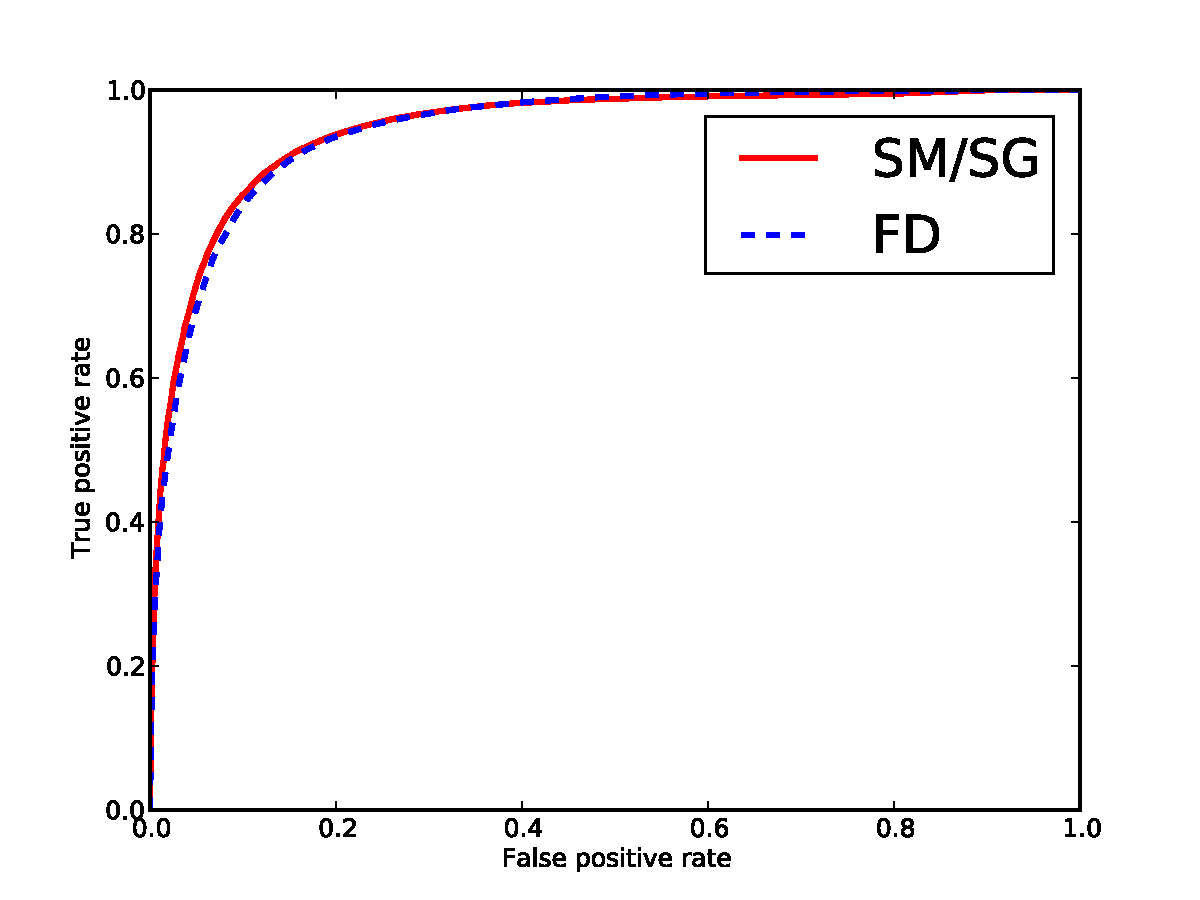
\includegraphics[width=1.7in]{SMSG_G_ep.pdf} 
&
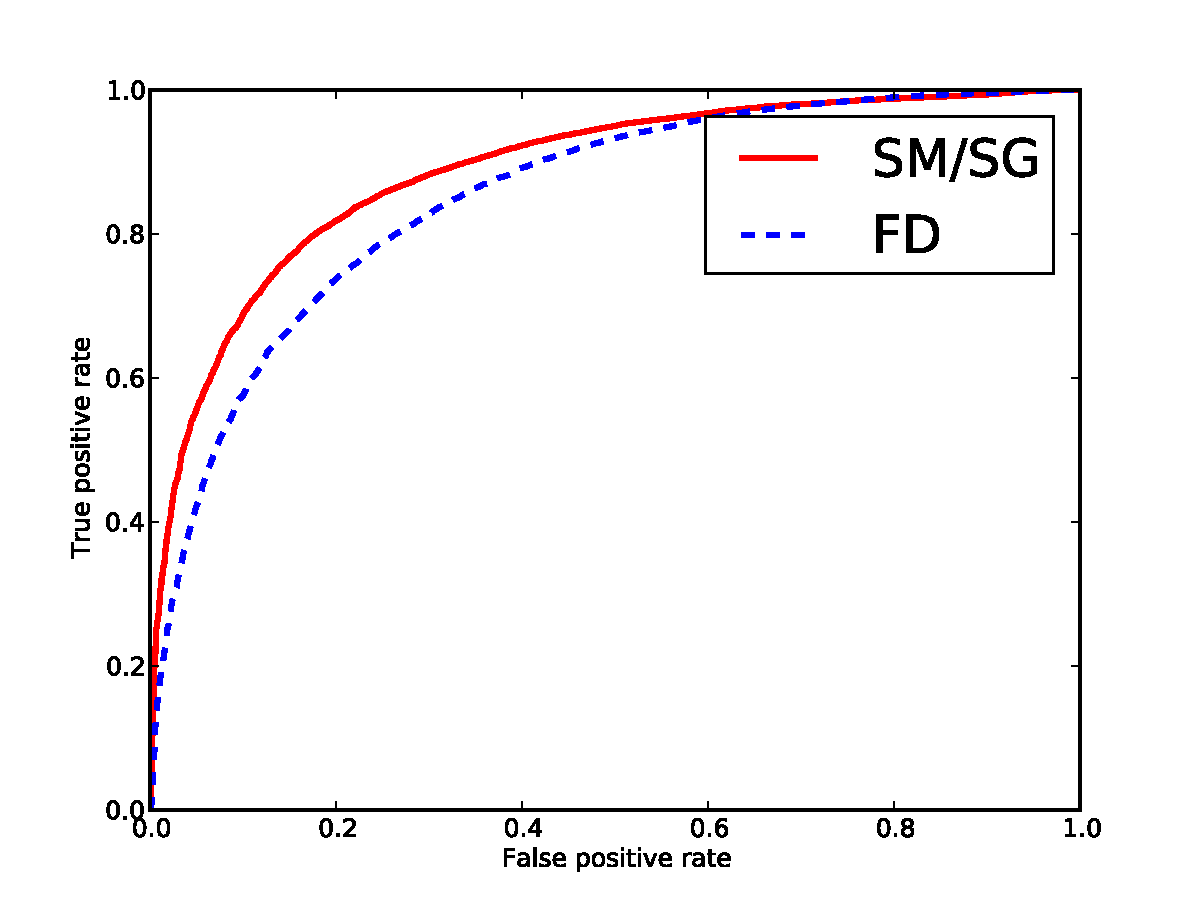
\includegraphics[width=1.7in]{SMSG_G_wiki.pdf} 
&
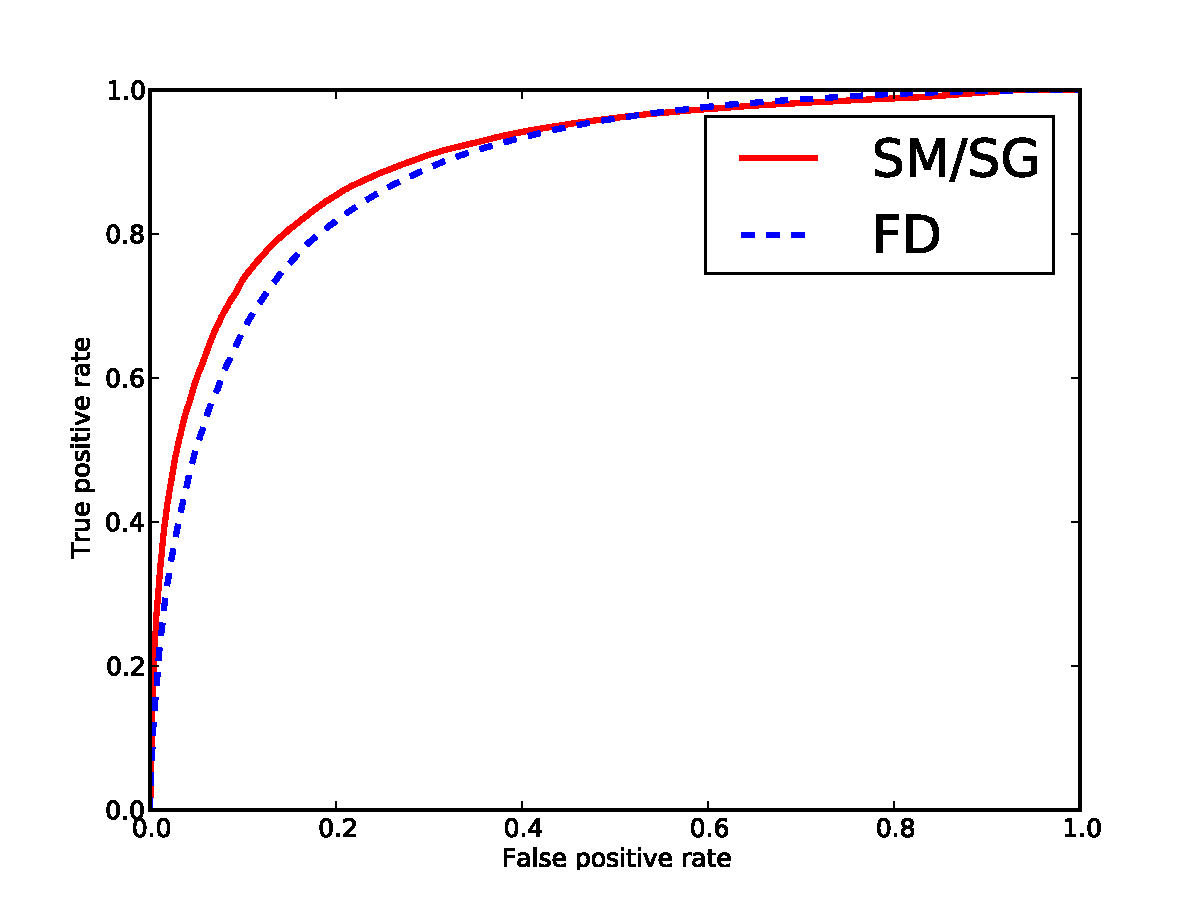
\includegraphics[width=1.7in]{SMSG_G_slash.pdf} \\
Epinions & Wikipedia & Slashdot
\end{tabular}}
\end{figure*}

\begin{table}[h]
\tbl{\label{tab:flipnumbers} Total number of edges in each class (S for
  single (S) edges and Bi for bi-directional edges) for Epinions using graph G.}{
\begin{tabular}{l|rrrrr} \\
Edges & S(+) & Bi(+) & S(-) & Bi(-) & Total \\ \hline
All trust edges & 465,350 & 249,614 & 116,271 & 4,731 & 835,966 \\
Flipped by SM/SG & 28,428 & 5,623 & 6,554 & 193 & 40,798 \\ 
Flipped by FD & 31,706 & 6,027 & 8,755 & 280 & 46,768 \\
\end{tabular}}
\end{table}



\subsection{External Validation} \label{sec:external}
In this section, we consider an external validation of our
methodology. Our algorithm solely considers the structural
information. However, additional information in the form of user
ratings of each other's reviews is available in the Epinions dataset
that can be used to validate the results of our algorithm. We showed
that our algorithm results in better prediction accuracy than
FD. However, there are various papers that report quite strong
prediction performance in Epinions such as
in~\cite{golbeck:distrust2011} by using structural information and
in~\cite{Tang:2013} by using homophily in the ratings. We believe this
is due to the fact that most distrust relationships in this dataset
are weak. As a result, fairly good prediction is possible even without
considering negative relations.

It is likely that most trust relationships in Epinions correspond to a
rating of competence (good/bad reviews) than untrustworthiness
(friend/enemy). When people judge competence, they consider
accumulation of positive evidence diagnostic. When somebody is
considered competent, their work is not scrutinized closely. However,
incompetent people are watched. If they perform well, trust for them
grows. As a result, even if a distrust rating exists, the relationship
may grow towards trust over time which should show up as improved
ratings for their articles. Structural balance in the network may
effect ratings in a few ways.  For example, suppose Alice distrusts
Bob, but other friends of Alice trust Bob. This may cause Alice to
have more opportunities to judge Bob as her friends promote Bob's
reviews. It is also possible that Alice starts to view Bob's reviews
more positively as she values her friends' judgment.  Our objective is
to check which algorithm captures this effect more accurately.

To test this, we first run both algorithms to find a converged version
of the training data as before. Our running hypothesis is that the
relationships were close to convergence before running the algorithm
and hence only a minimal set of relations will change sign after
convergence. Using the test cases, we determine the threshold that
gives the best separation between positive and negative
predictions. Based on these predictions, we now consider which edges
in the {\em training set} have flipped their sign after
convergence. In other words, flipped edges after convergence were
those edges that were most likely to change sign according to a
specific algorithm. We compare the flipped edges from the training set
for both algorithms SM/SG and FD in Tables~\ref{tab:flipnumbers}
and~\ref{tab:reviews}. Note that in this case, we are only reporting
on edges that are either single directional or bi-directional with the
same sign. The number of edges in each category follow a similar
pattern in SM/SG and FD, but fewer edges are flipped in SM/SG. This is
expected as FD does not operate on an explicit constraint to preserve
the network relations as much as possible.  The more important
question is if there is a difference in the characteristics of the
flipped edges. For these, we look at the ratings Alice gave to Bob
{\em after she reported on her trust rating}. These are given on the
right side of the table.

We first look at the overall trend, if Alice trusts Bob, she also
gives her overall higher rating values (4.60/4.76 for S(+)/Bi(+)
edges) than if she distrusts him (3.76/3.32 for S(-)/Bi(-)
edges). Furthermore, after the trust rating is given, the review
ratings for trusted people go up (4.98/4.99) and distrusted people
goes down (3.20/3.40). We can also see that for bi-directional edges,
trusted people have higher ratings (4.76 versus 4.60) and distrusted
people have lower ratings (3.32 versus 3.76).  This shows the
correlation between trust ratings and reviews, as well as
justification to treat bi-directional edges as stronger relationships.

How about the people who were flipped by the different algorithms (see
Table~\ref{tab:reviews})? For both algorithms, the flipped people had
overall slightly lower positive ratings, which might signal that the
overall strength of positive relationships were not as high as the
average link. There is no difference in the ratings after the trust
edge is created. Hence, the reviews become more positive after the
rating for flipped edges as well. This could just be the norm for this
data set. 

The distinction becomes clear in the negative edges.  For both
algorithms, the flipped negative edges (i.e. those that have become
positive) have higher ratings after the trust rating is given when
compared to the full data. But this effect is much more pronounced in
SM/SG in all cases: flipped S(-) edges have average rating of 4.13 as
opposed to the overall average 3.76, and the ratings for these edge go
up to 4.41 after the rating is given. Similarly, Bi(-) edges have
weight 3.75 as opposed to the general average of 3.32, and they go up
to 3.93 after convergence. In contrast, the ratings for the flipped
Bi(-) edges according to FD go down after the rating is given. Hence,
the edges made positive by FD actually become more negative according
to ratings. As a result, the rating information does not support
convergence hypothesis for FD, but it strongly supports it for
SM/SG. SM/SG is able to better capture the expected change in
relationships by finding negative edges that are weak overall and that
have evolved towards a more positive relationship over time. In fact,
the structural information and stress in relations provide significant
information that can be used to predict such change. Note that for
this experiment, we are treating all edges the same to obtain a fair
comparison with FD that does not consider edge strength. In
Section~\ref{sec:tiestrength}, we will look at prediction when
considering edge strength as well.

\begin{table}[h]
\tbl{\label{tab:reviews} Average value of ratings along a specific
  type of trust edge in the whole Epinions dataset and after the trust
  edge was created (S for single (S) edges and Bi for bi-directional
  edges). For each edge, the average ratings for that edge is
  considered, and then the value is averaged for the specific group of
  edges. Results based on graph G.} {
\begin{tabular}{l|llll|llll} 
\multicolumn{1}{c}{} & \multicolumn{4}{c}{Average rating value} &
  \multicolumn{4}{c}{Average rating value after} \\ 
\multicolumn{1}{c}{} & \multicolumn{4}{c}{} &
  \multicolumn{4}{c}{trust edge is created} \\ 
Edges & S(+) & Bi(+) & S(-) & Bi(-) & S(+) & Bi(+) & S(-) & Bi(-)  \\ \hline
All trust edges & 
4.60 & 4.76 & 3.76 & 3.32 & 4.98 & 4.99 & 3.20 & 3.40 \\
Flipped by SM/SG &
4.43 & 4.80 & 4.13 & 3.75 & 4.98 & 5.00 & 4.41 & 3.93 \\
Flipped by FD & 
4.42 & 4.81 & 4.03 & 3.63 & 4.99 & 5.01 & 4.39 & 3.32 \\
\end{tabular}}
\end{table}



\begin{figure*}[thbp!]
\tbl{\label{fig:expand}The ROC curves are drawn upon distances of
  hidden edges, generated by SM/SG and FD for G$^{\#}$ given Slashdot
  and Wikipedia datasets. Area under the curve of (SM, FD)
  for Wikipedia: ({\bf 0.832}, 0.850), and Slashdot: ({\bf 0.900},
  0.838).}{
\begin{tabular}{cc}
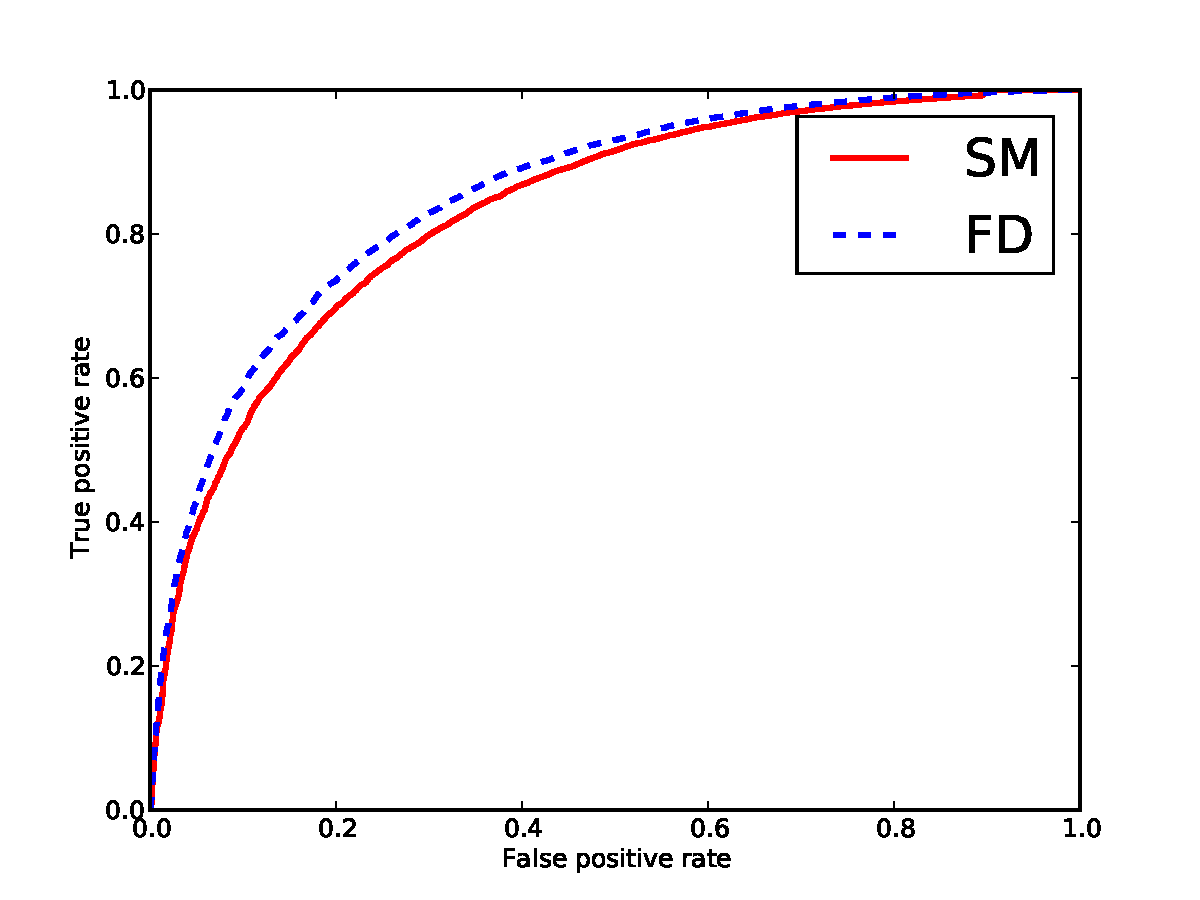
\includegraphics[width=1.7in]{SMSG_Gsharp_wiki.pdf} 
&
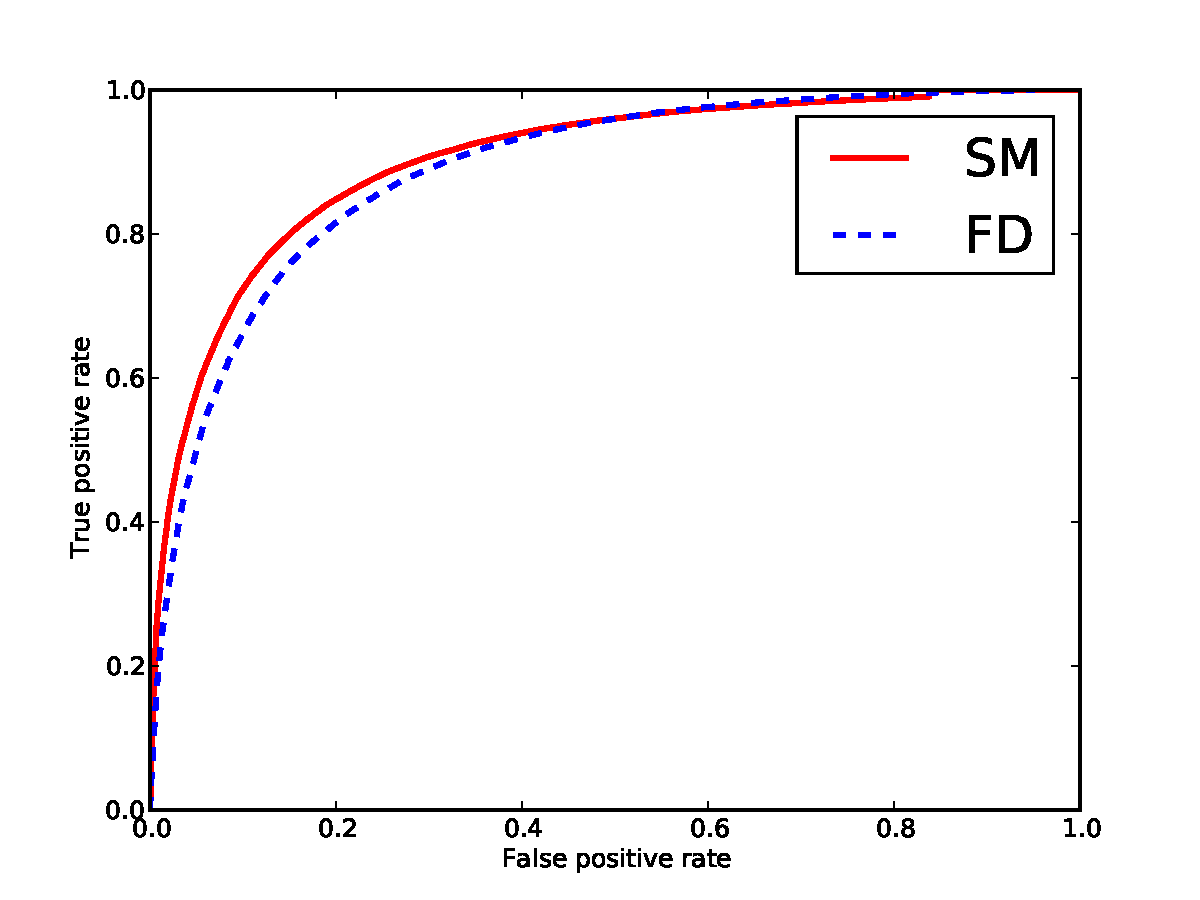
\includegraphics[width=1.7in]{SMSG_Gsharp_slash.pdf} \\
Wikipedia & Slashdot
\end{tabular}}
\end{figure*}


\subsection{Impact of Indirect Neutral Edges} \label{sec:indirect-neutral}
As we have seen earlier with the sampled graphs, disregarding unknown
neutral edges by using SM/SG does not result in a performance
penalty. The question is whether there is a better definition of
neutral edges. Instead of considering all unknown edges as neutral, we
can restrict neutral edges to those pairs who have a chance to know
each other. We define this as pairs of nodes for which the shortest
path between them is of length 2.  This is given in graph G$^\#$.  In
the resulting graphs, the expanded Epinions has around 70 times its
original size, the expanded Slashdot has around 23 times its original
size and the Wikipedia has around 15 times its original size. Due to
its large size, running SM/SG on Epinions is not feasible. We only
report on Wikipedia and Slashdot.

We compare the performance of SM/SG to FD in
Figure~\ref{fig:expand}. The performance of FD is the same as it is
for G since it does not consider neutral edges. The performance is
slightly worse in Wikipedia. In fact, this is the only case SM/SG does
worse than FD. If (A,B) and (A,C) are both weak ties, then it is very
likely that the existence of these ties would have an effect on the
relationship between (A,C). Hence, adding such a relationship as a
neutral edge is likely to hurt performance. We hypothesize that this
is the reason for the reduced performance. In fact, despite the
relatively small percentage of edges added, Wikipedia is the worst
effected from this change. A reasonable conclusion in this case is
that Wikipedia data set has the highest concentration of weak edges.
Given Wikipedia is based on voting, the relationships have a more
hierarchical and organizational flavor than the other datasets. This
might explain why the relationships between voters (incumbents) and
those who are voted on (newcomers) are mostly weak relationships.


\subsection{Coverage} \label{sec:coverage}
We now consider the accuracy of prediction by removing 10\%, 30\%,
50\%, 70\% and 90\% of the edges. The remaining edges are used as the
training set, and the removed edges are used as the testing
set. Notice that there are edges in the testing set with endpoints
that are not shown in the training set. We cannot predict such edges
because the locations of the untrained endpoints are unknown. We
simply ignore such edges in testing. Again, we employ 10-fold
validation for each experiment. The results are shown in
Figure~\ref{fig:accuracy_test}. In all data sets, the prediction
remains quite high even when we remove 10\%-50\% of the edges. There
is slight degradation at 70\%, and a much higher drop at 90\%. At
90\%, the prediction is around 83.7\%, 71.8\% and 73.4\% on Epinions,
Wikipedia and Slashdot respectively at the best cut-off. The
degradation is better than reported in~\cite{golbeck:distrust2011}. We
also note that Wikipedia and Slashdot are impacted more by this
change, as prediction is harder for these data sets.

\begin{figure*}[thbp!]
\tbl{\label{fig:accuracy_test}The ROC curves are drawn upon distances of
  hidden edges after removing 10\%, ..., 80\% of the edges
  correspondingly, generated by SM/SG for G given Epinions, Slashdot
  and Wikipedia datasets. }{
\begin{tabular}{ccc}
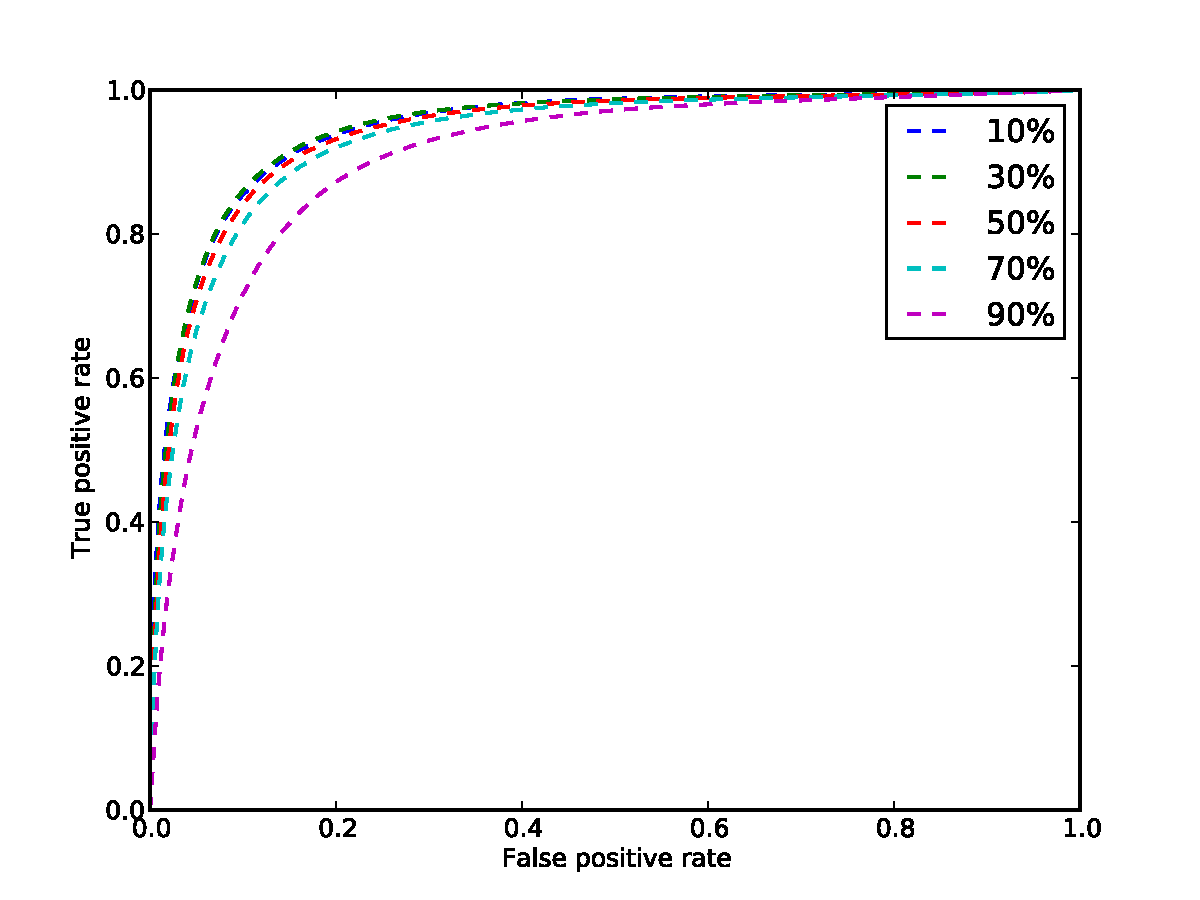
\includegraphics[width=1.7in, height=1.3in]{per_ep.pdf} 
&
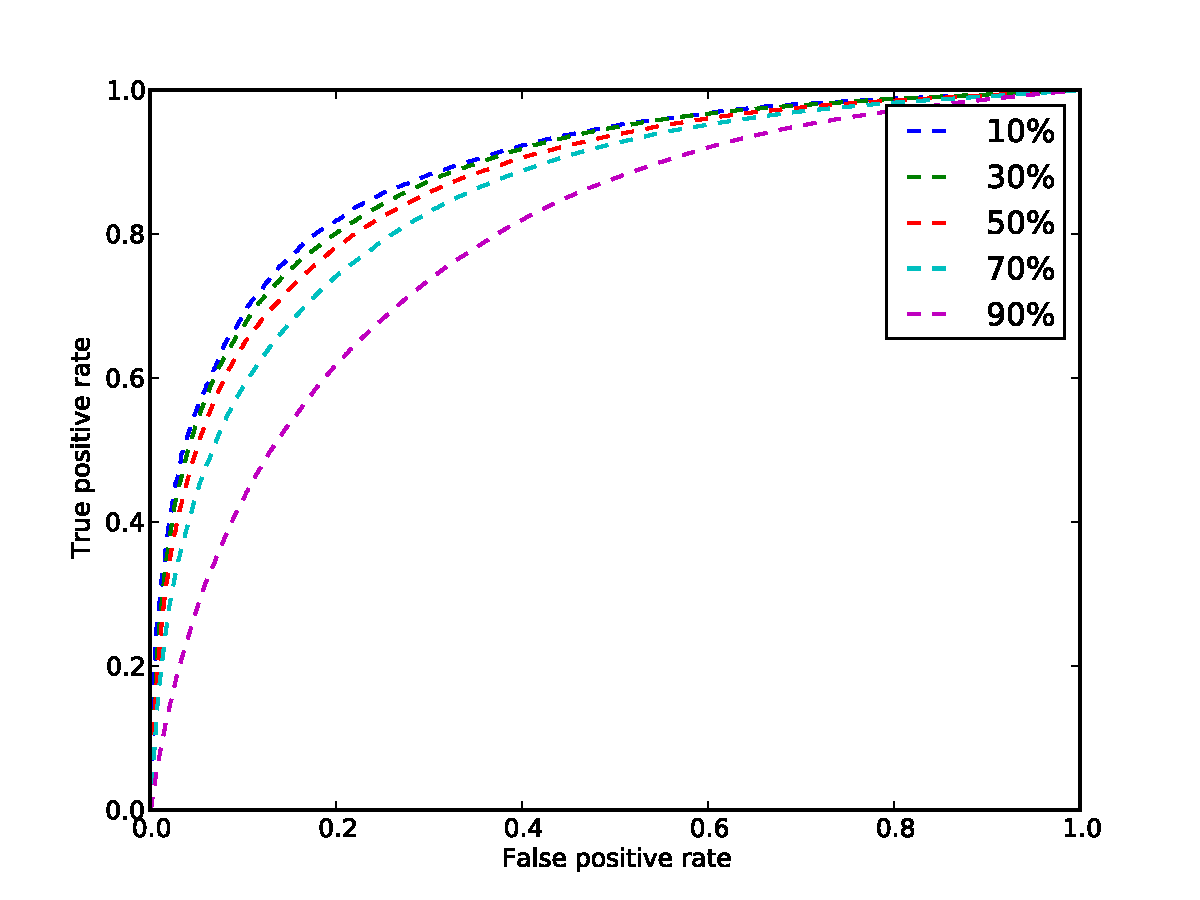
\includegraphics[width=1.7in, height=1.3in]{per_wiki.pdf} 
&
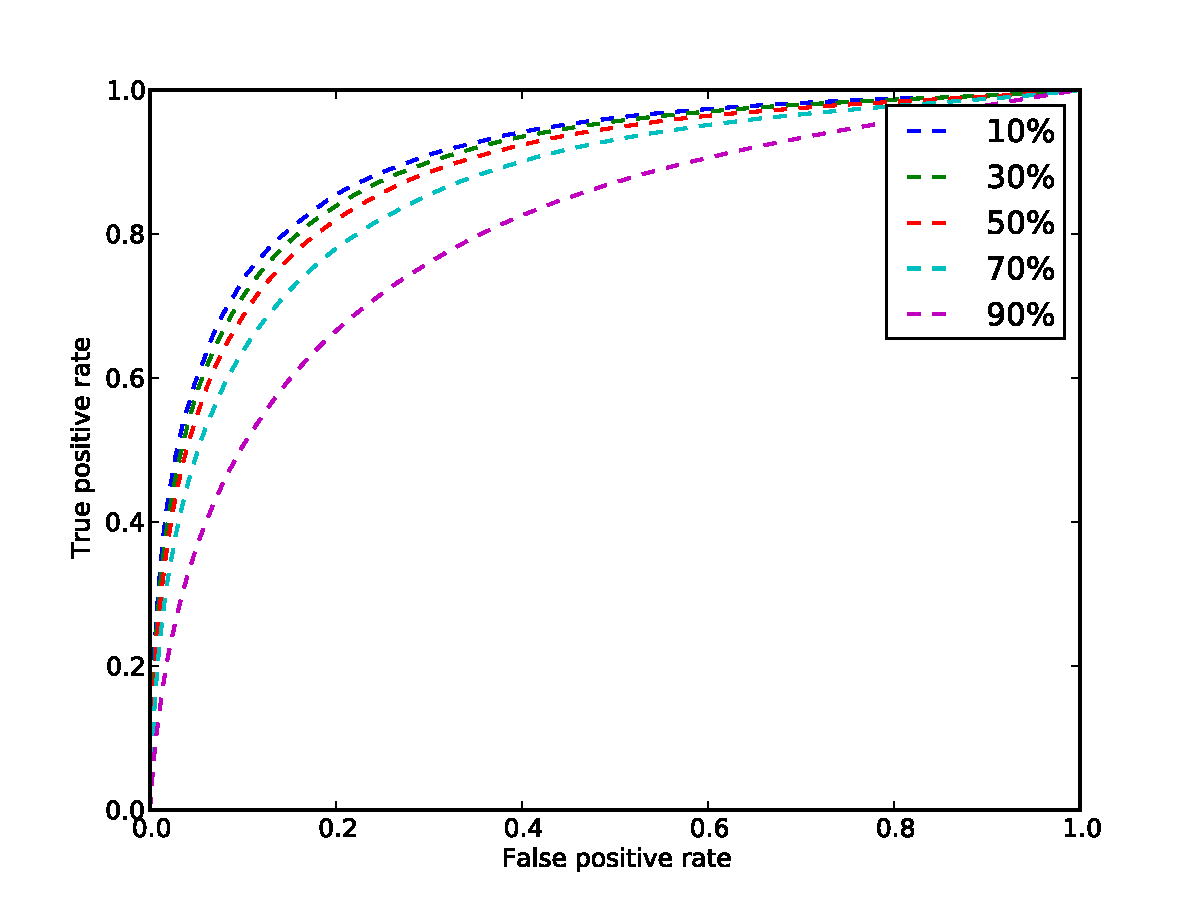
\includegraphics[width=1.7in, height=1.3in]{per_slash.pdf} \\
Epinions & Wikipedia & Slashdot
\end{tabular}}
\end{figure*}


\subsection{Effect of Time} \label{sec:results-time}
In this section, we consider the accuracy of our algorithm in
predicting the future. In other words, given the relations as they
exist in the database right now, what will be the relations for the
newcomers? This is a slightly harder problem. Newcomers are unlikely
to have many connections to the existing network. They are also
very unlikely to link to each other. To test this, we take the first
90\% of the edges in Epinions as the training set, and use the
remaining as the test case. In Wikipedia, we take the first 90\% of
the elections as training set, and the remaining as the test set. As
there is no time information in Slashdot, we are unable to apply this
test to this dataset. The results are given in
Figure~\ref{fig:last10}. The prediction is worse than random removal
case. In fact, it is almost random choice for Wikipedia. But SM/SG
does better than FD in both data sets. This is a case in which
additional information like homophily based on reviews can be expected
to make a big difference in improving the accuracy of predictions.

\begin{figure*}[thbp!]
\tbl{\label{fig:last10}The ROC curves are drawn upon distances of
  hidden edges after removing the {\bf last} 10\% with respect to time
  of the edges in Epinions and Wikipedia, generated by SM/SG for G.
  Area under the curve of (SM/SG, FD) for Epinions: ({\bf 0.814},
  0.785) and Wikipedia: ({\bf 0.710}, 0.675).}{
\begin{tabular}{cc}
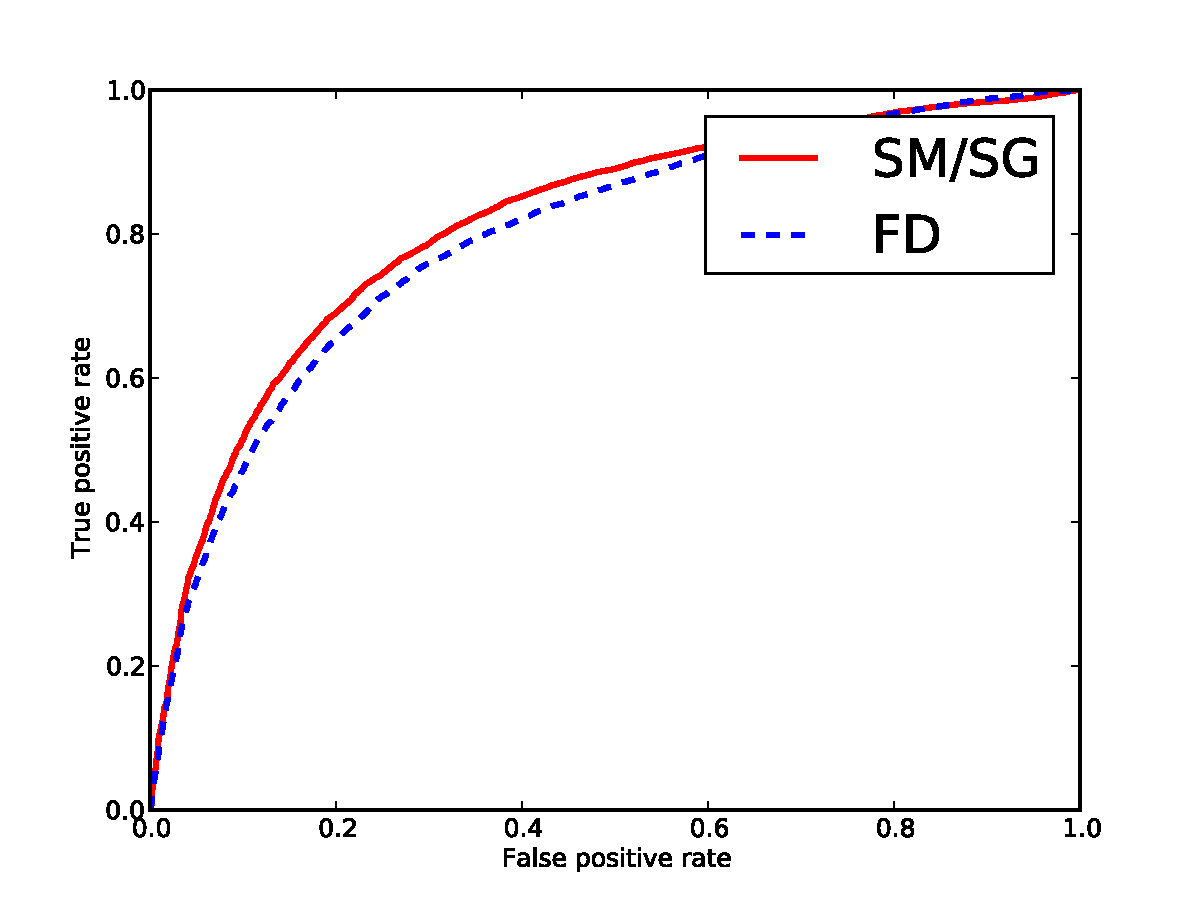
\includegraphics[width=1.7in, height=1.3in]{last10_ep.pdf} &
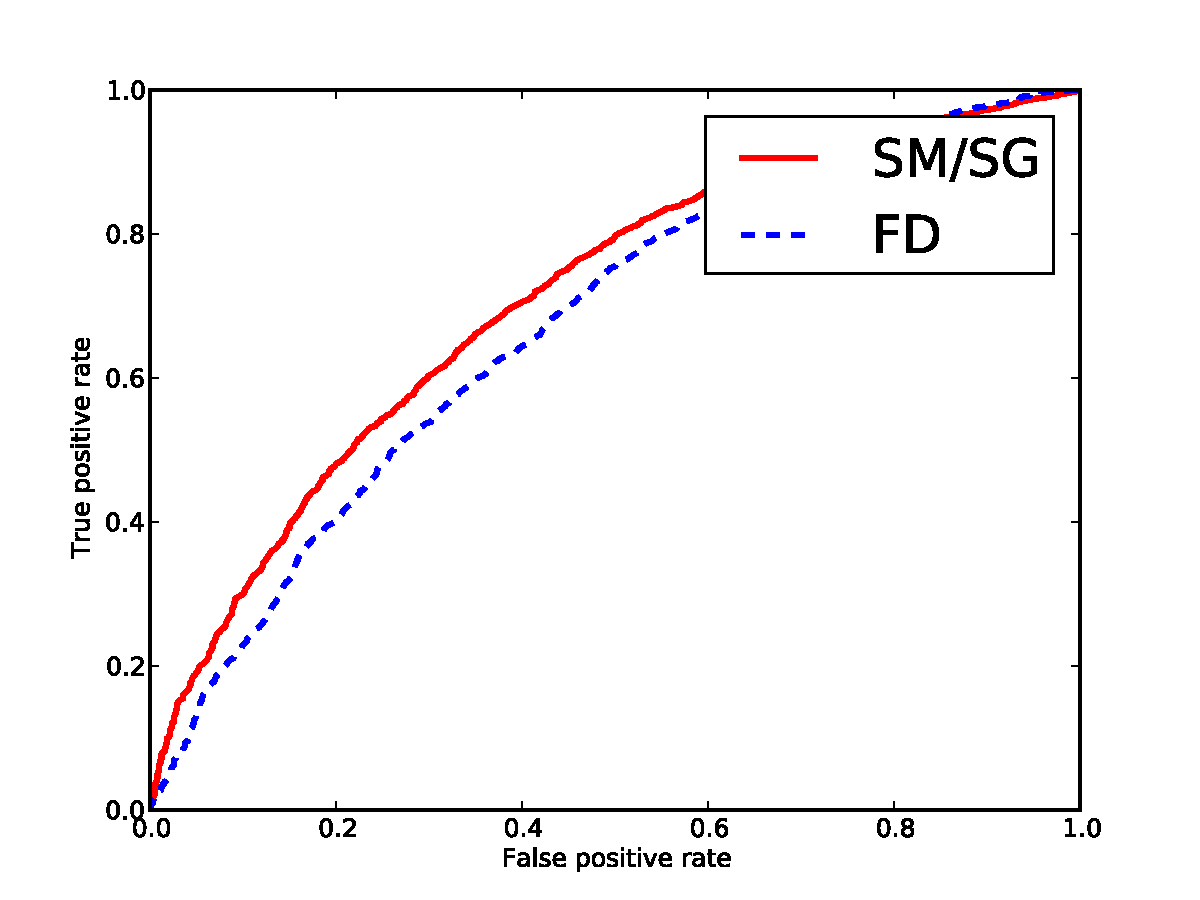
\includegraphics[width=1.7in, height=1.3in]{last10_wiki.pdf} \\
Epinions & Wikipedia
\end{tabular}}
\end{figure*}




\begin{figure*}[thbp!]
\tbl{\label{fig:coms}The ROC curves are drawn upon distances of hidden
  bi-directional edges in G-di, generated by SM/SG and FD on different
  graphs, given Epinions, Wikipedia, and Slashdot datasets. Area
  under the curve of (SM/SG:G-di, SM/SG:G-bi, SM/SG, FD, FD:G-bi) for
  Epinions: ({\bf 0.956}, 0.953, 0.946, 0.932, 0.855), Wikipedia:
  ({\bf 0.943}, 0.895, 0.911, 0.857, 0.788), and Slashdot: ({\bf
    0.939}, 0.909, 0.904, 0.888, 0.825).}{
\begin{tabular}{ccc}
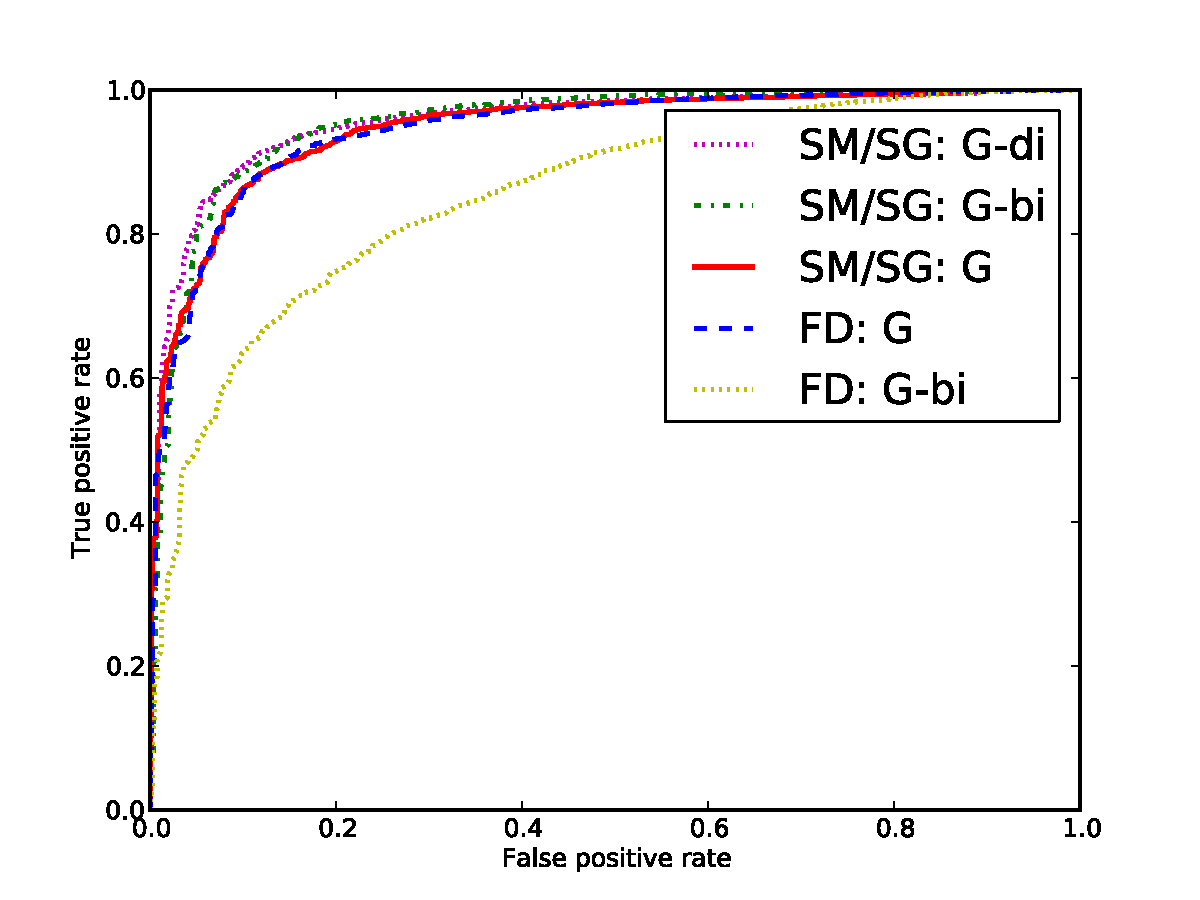
\includegraphics[width=1.7in, height=1.3in]{Com_Gdi_ep.pdf} 
&
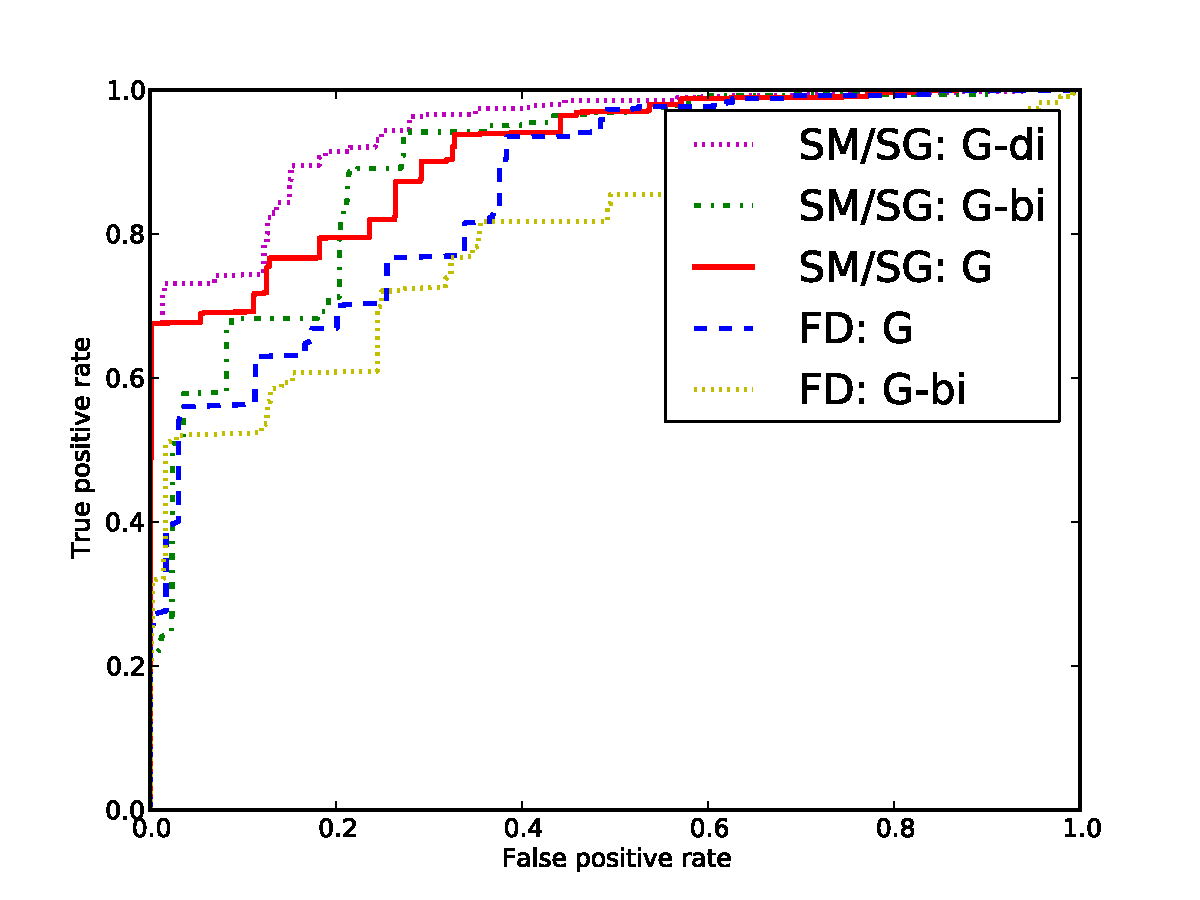
\includegraphics[width=1.7in, height=1.3in]{Com_Gdi_wiki.pdf} 
&
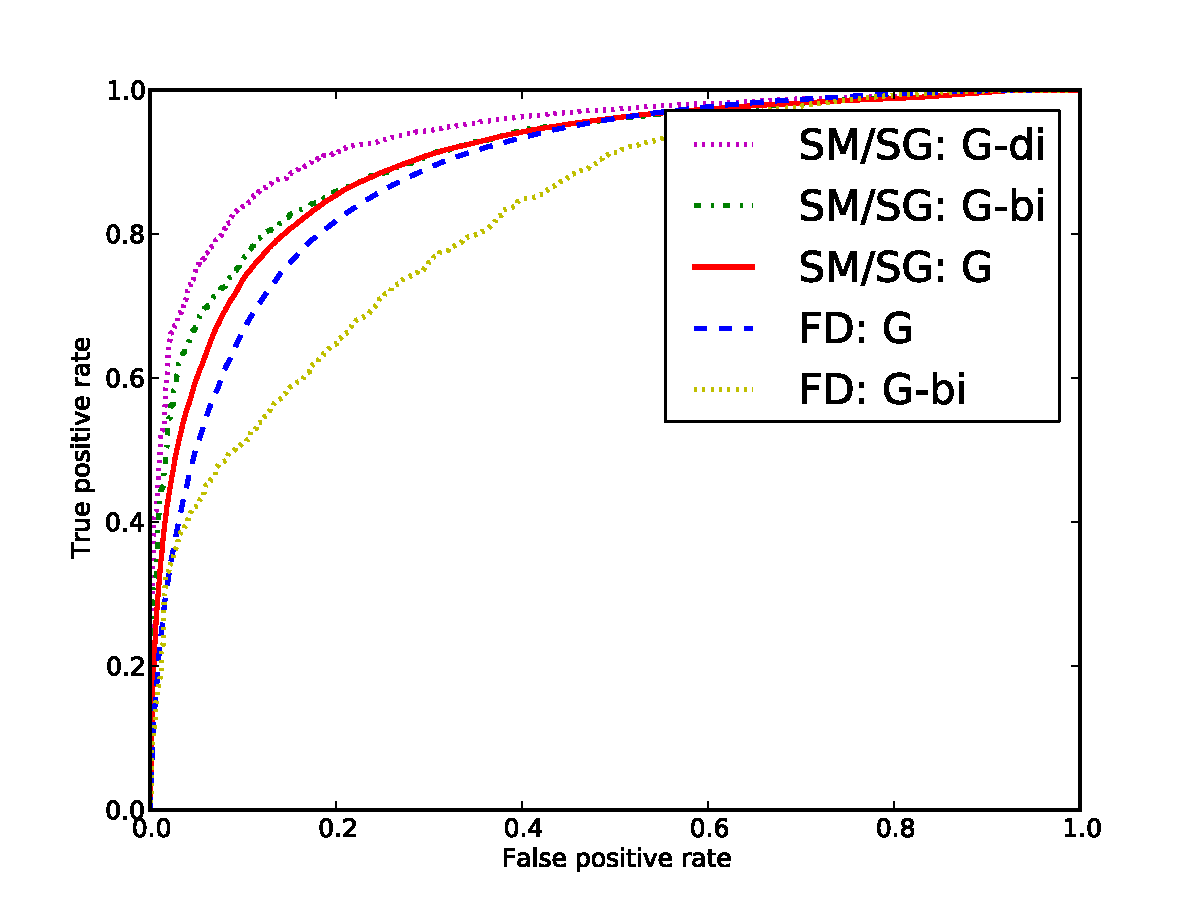
\includegraphics[width=1.7in, height=1.3in]{Com_Gdi_slash.pdf} \\
Epinions & Wikipedia & Slashdot
\end{tabular}} 
\end{figure*}


\begin{figure*}[thbp!]
\tbl{\label{fig:comd}The ROC curves are drawn upon distances of hidden
  edges of all types in G-di, generated by SM/SG and FD on different
  graphs, given (1) Epinions, (2) Slashdot and (3) Wikipedia
  datasets. Area under the curve of (SM/SG:G, FD, SM/SG:G-di) for
  Epinions: ({\bf 0.947}, 0.946, 0.941), Wikipedia: ({\bf 0.888},
  0.849, {\bf 0.888}), and Slashdot: ({\bf 0.905}, 0.888, 0.888).}{
\begin{tabular}{ccc}
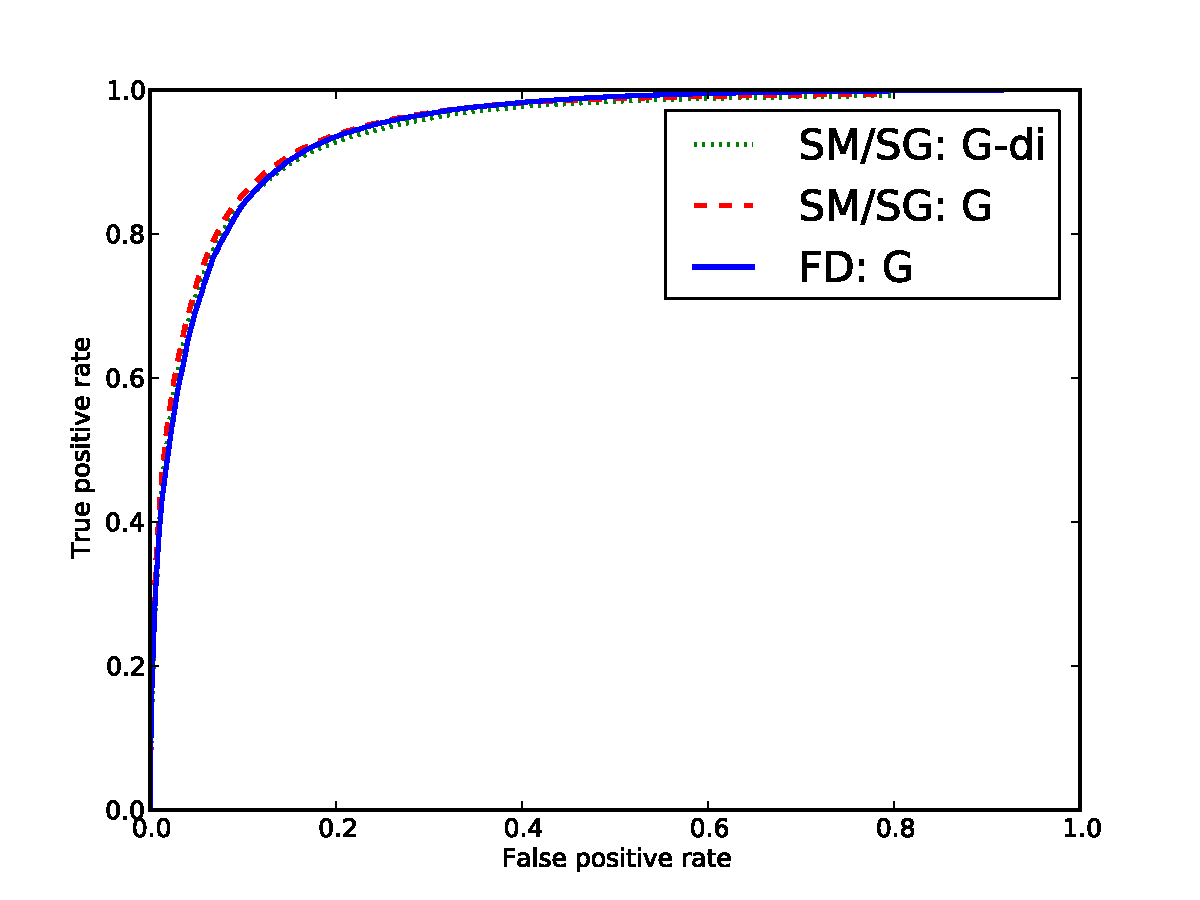
\includegraphics[width=1.7in, height=1.3in]{Com_all_ep.pdf} 
&
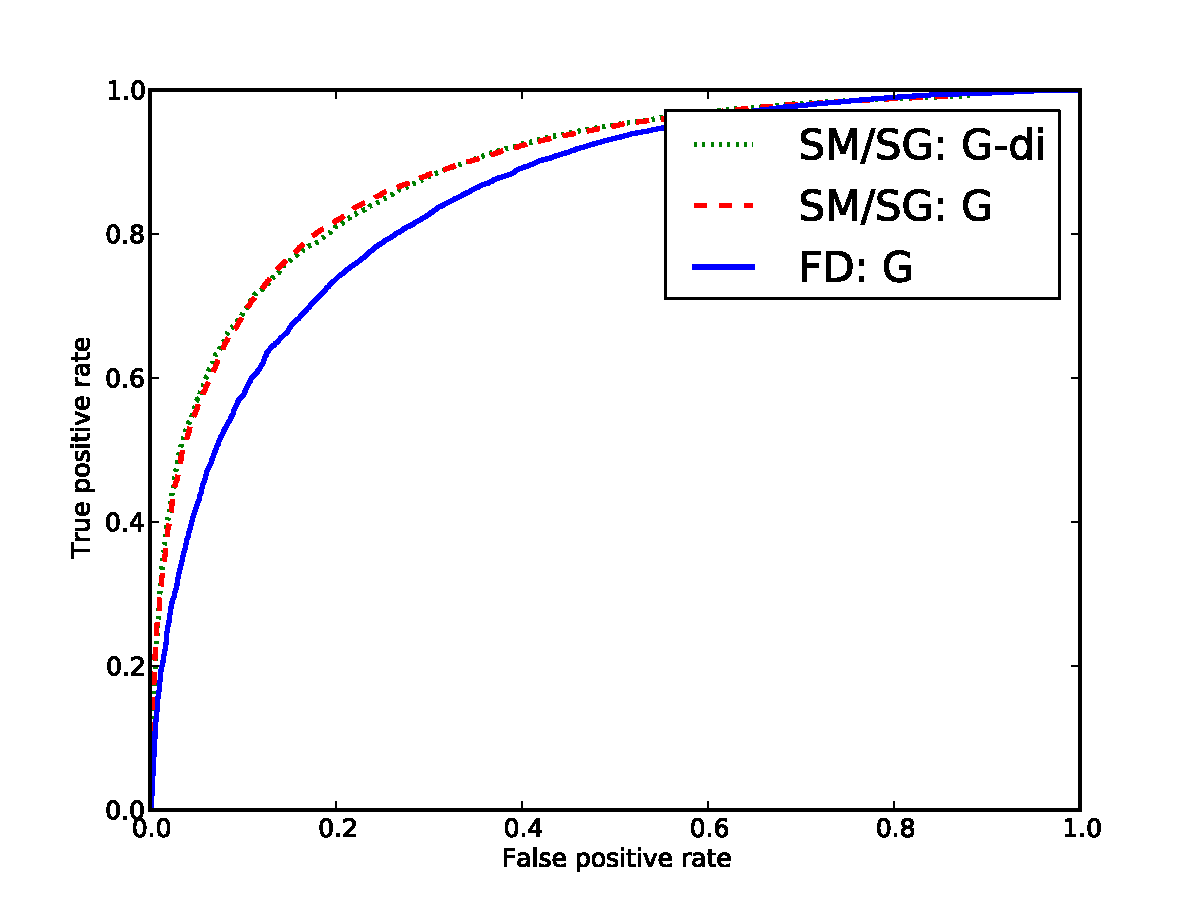
\includegraphics[width=1.7in, height=1.3in]{Com_all_wiki.pdf} 
&
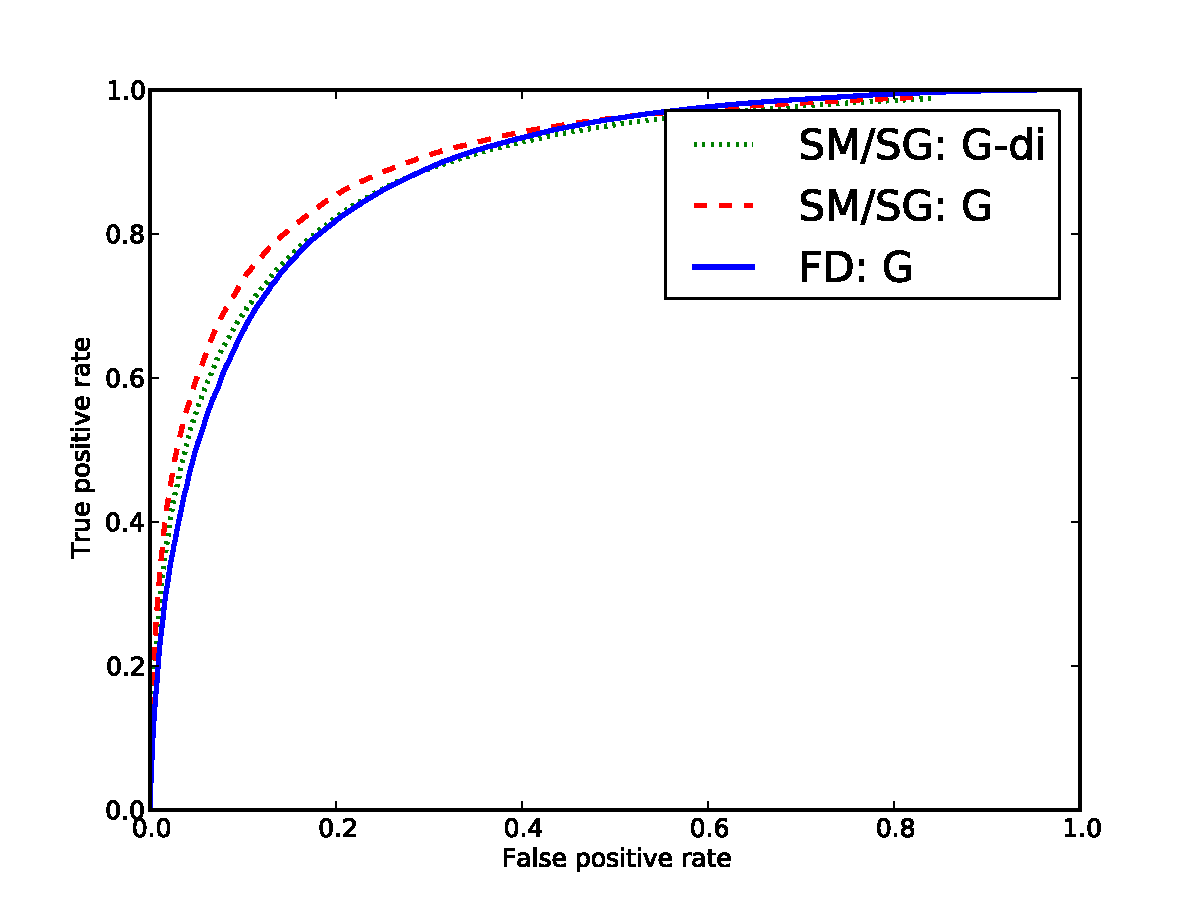
\includegraphics[width=1.7in, height=1.3in]{Com_all_slash.pdf} \\
Epinions & Wikipedia & Slashdot
\end{tabular}}
\end{figure*}

\subsection{Impact of considering weak and strong edges} \label{sec:tiestrength}
We repeat the experiments by considering strong and weak ties. We
check whether it leads to an increased performance using different
graphs. In particular, bi-directional edges are considered to be of
strong strength and are assigned with large weights while single
directional edges are considered to be of weak strength and are
assigned with small weights. In our practice, we set the weight of a
strong edge to be 10 times the weight of a weak edge. 

As it is shown in Figure~\ref{fig:coms}, we first compare the
prediction performance on testing samples consisting of {\bf
  bi-directional edges only} in different graphs.  For all three
datasets, we find SM/SG on G$-di$ has consistently the best
performance, followed by SM/SG on G$-bi$, SM/SG on G, FD on G and FD
on G-$bi$. In Wikipedia, the variance of the prediction is relatively
big because the testing sample is small ($n \approx 3000$). As argued
earlier, relationships based on voting do not naturally lend
themselves to bi-directional edges. But, even in this case, the
existence of votes of the same type in both directions lend themselves
to a dramatic improvement in the prediction of bi-directional edges.

At the best thresholds, SM/SG on G$-di$ achieves $90\%-91 \%$ accuracy
for Epinions, $87\%-88 \%$ accuracy for Slashdot and $84\%-85 \%$
accuracy for Wikipedia on both positive and negative hidden edges. On
the one hand, the fact that SM/SG on both G$-di$ and G$-bi$ have
better performance than it is on G implies that bi-directional edges
are indeed of strong strengths, which provide significant influence on
network convergence. On the other hand, the superior performance of
SM/SG on G$-di$ indicates that both strong and weak ties influence the
convergence, and that our convergence model provides an accurate way
to model such combined influence.

We repeat the comparing experiments on testing samples consisting of
both bi-directional edges and single directional edges. As it is shown
in Figure~\ref{fig:comd}, SM on G$-di$ does not give better
predictions than it is on G. As the single directional edges are
assigned with small weights, their influences on convergence is
weakened which impacts the prediction accuracy negatively. Considering
the fact that single directional edges are the dominant majority in
all three datasets, it is reasonable to see compromised overall
prediction performance.

We note however that while the number of positive edges is about 3.5-5
times the number of negative edges overall, the number of strong
positive edges to the number of negative edges is much more
unbalanced. Mutual hatred is generally uncommon. For example, in
Epinions, the ratio of strong positive edges to strong negative edges
is 50. Hence, both the prediction and the convergence is strongly
effected by the strong positive edges as a result. This could be the
reason behind the poor performance of FD on G$-bi$ that relies only on
the strong edges. We repeat the same ground truth comparison that was
shown in Table~\ref{tab:reviews} of Section~\ref{sec:external} for
Epinions, this time for G-bi, using the strong edges to determine the
optimal threshold. The comparison is shown in
Table~\ref{tab:reviews-di}. The results remain almost the same except
there is a slight improvement in all cases except for the strong
negative edges. A possible way to counteract the effects of such an
imbalance is to increase the weights of strong negative edges.

\begin{table}[h]
\tbl{\label{tab:reviews-di} Average value of ratings along a specific
  type of trust edge in the whole dataset and after the trust edge was
  created (S for single (S) edges and Bi for bi-directional
  edges). Comparing SM/SG on G and G-di.} {
\begin{tabular}{l|llll|llll} 
\multicolumn{1}{c}{} & \multicolumn{4}{c}{Average rating value} &
  \multicolumn{4}{c}{Average rating value after} \\ 
\multicolumn{1}{c}{} & \multicolumn{4}{c}{} &
  \multicolumn{4}{c}{trust edge is created} \\ 
Edges & S(+) & Bi(+) & S(-) & Bi(-) & S(+) & Bi(+) & S(-) & Bi(-)  \\ \hline
Flipped by SM/SG on G-di & 
4.46 & 4.82 & 4.17 & 3.71 & 4.99 & 5.01 & 4.48 & 3.49 \\
Flipped by SM/SG on G &
4.43 & 4.80 & 4.13 & 3.75 & 4.98 & 5.00 & 4.41 & 3.93 \\
\end{tabular}}
\end{table}



\begin{figure*}[thbp!]
\tbl{\label{fig:weight_change}The ROC curves for Slashdot. SM/SG:5
  corresponds to a run in which strong edges have 5 times the weight
  of weak edges, and SM/SG:10 corresponds to 10 times accordingly.}{
\begin{tabular}{cc}
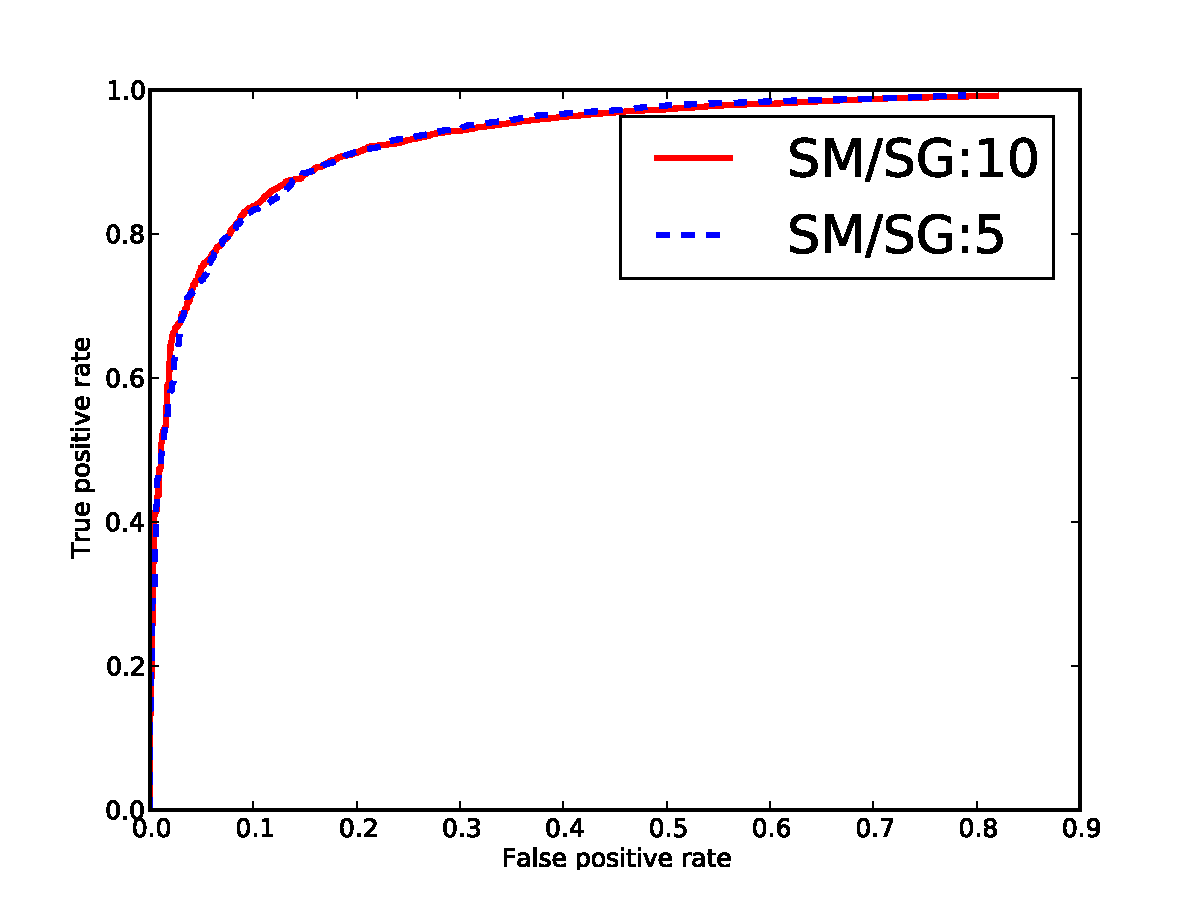
\includegraphics[width=1.7in, height=1.3in]{SMSG5_slash.pdf} &
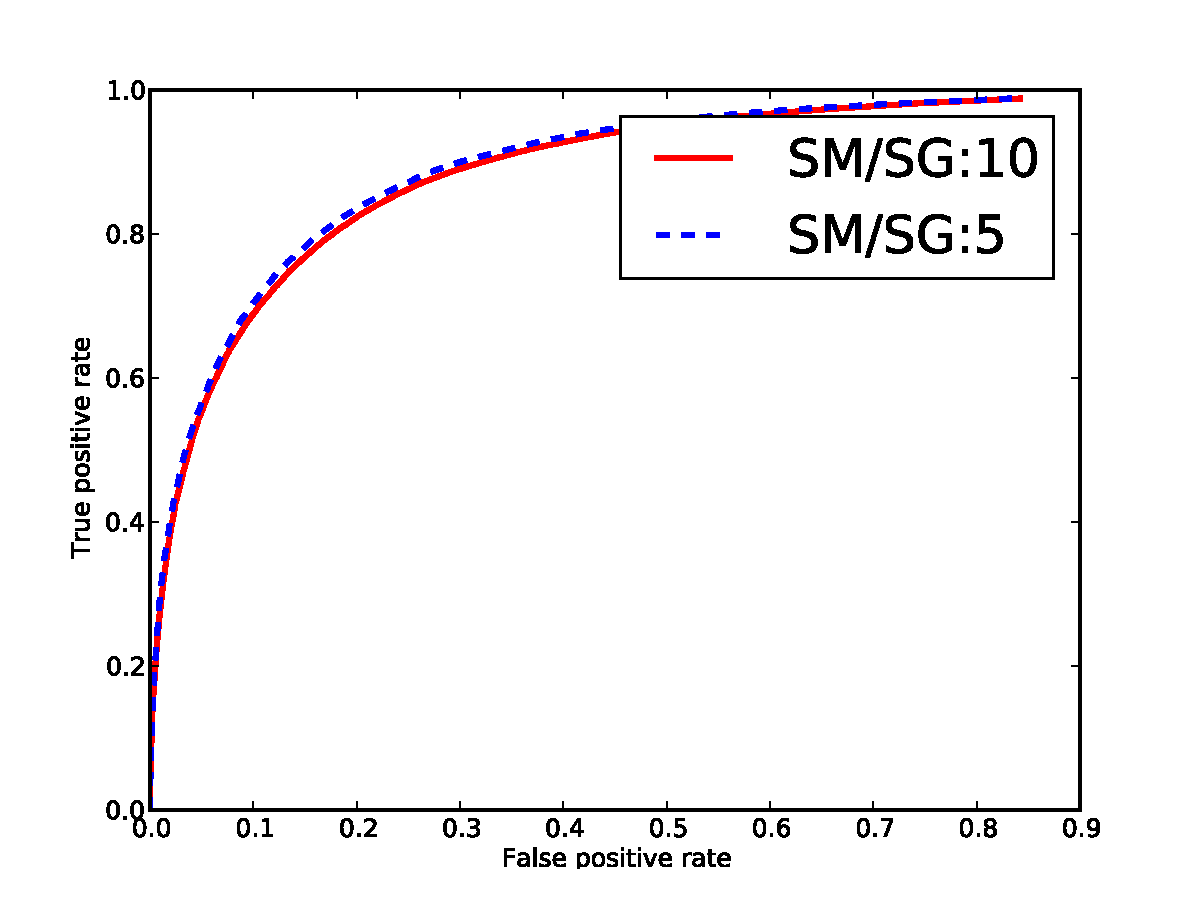
\includegraphics[width=1.7in, height=1.3in]{SMSG5_slash_di.pdf} \\
(a) Bi-directional edge prediction on G-di & (b) All edge prediction
on G-di
\end{tabular}}
\end{figure*}

\subsection{Sensitivity to parameter choice} \label{sec:sensitivity}
In the previous sections, we have presented a number of results with a
specific collection of parameters. In this section, we discuss briefly
to which degree the algorithm depends on the selection of these
parameters. 

We have run our algorithm with various combinations of weights. Even
though the weights provide an adjustable parameter for our algorithm,
the results do not change considerably in response to small weight
changes (e.g. setting $w_{-}=w_{+}$). However, $w_{O}$ must be set to
a much smaller value ($w_{O}<< w_{-}, w_{+}$), otherwise neutral edges
have too much influence in the results. These neutral edges are very
noisy as most correspond to pairs who do not know each other. In fact,
SM/SG assigns zero weights to these edges without significant
penalty. 

Note that by significantly changing the weights, it is possible to
favor the influence of positive relations over negative, and vice
versa.  It is also possible to tune the weights in SM/SG at the edge
level by incorporating prior information about the underlying
network. It is not obvious how such changes can be applied to FD in a
principled way and without jeopardizing converge. To illustrate the
effect of changes in weight, we run a comparison between two different
versions of assigning weights to edges with strong ties. In SM/SG:5,
the strong ties have five times the weight as weak ties, and in
SMS/SG:10, strong ties have 10 times the weight as weak ties (our
original setting). The comparison is shown in
Figure~\ref{fig:weight_change}. We only show slashdot for brevity, but
the other results are similar. We note that by lowering the weight of
strong edges to 5 times, the strong edge prediction gets slightly
worse, but the general edge detection improves slightly. Hence, the
weights provide a way to influence which factors the algorithm should
prioritize.

We have also investigated the importance of changing the initial
values for distances.  We have argued that the initial distances
should at least satisfy: $d_{+} < \frac{d_{O}}{2} < \frac{d_{-}}{2}$ where
$d_{+}$, $d_{O}$, $d_{-}$ are original distances of a positive edge, a
neutral edge and a negative edge. We have run tests on $0.1,0.6,1.1$,
$0.1,0.3,0.9$ and $0.05,0.5,2.0$ for $d_{+}, d_{O}, d_{-}$.  The
prediction curves remained identical. Overall, the algorithm is not
sensitive to the constraints for positive and negative distances as
long as the overall above relationship between the distances are
preserved.

\subsection{General Link Prediction.} \label{sec:link-prediction}
We finish this section by discussing a different application of our
framework and algorithm. So, far we have been discussing the {\it edge
  sign prediction} which deals with the cases in which we already know
that an edge exists in the original network. A more general and harder
problem is to predict whether there is a positive or a negative edge
between a pair of nodes (link prediction~\cite{Kleinberg:03}). The
difficulty of these problems stem from the fact that large social
networks are not only sparse and are incomplete, but most of the edges
in such networks are of weak strength that do not convey much useful
information. Our convergence model should be able to make general edge
predictions based on distances. If larger distances represent more
negativeness (less positiveness), then the distance of a neutral
relation should be smaller than a negative one and larger than a
positive one. As a consequence, the distribution of neutral edges in
terms of distance should concentrate in the middle range. We study
this distribution, as a preliminary step towards solving the general
edge prediction.

For each dataset, we generate samples based on random source nodes as
in samples of G$^*$ we have studied earlier, except that we exclude
the edges between the $k$ source nodes. Instead of cross validation,
we use the entire sub-network for training, and use the $k(k-1)/2$
edges between the $k$ source nodes as testing data, whose signs are
available in the original dataset (positive, negative or neutral,
i.e. no link). 
After convergence the distances of these edges should be
representative of their true signs. We repeat the experiments 50 times
over all three datasets, and collect the distances for only the
neutral testing edges. Figure~\ref{hist} shows that the distances of
neutral testing edges generated by SM do relatively concentrate in the
middle-range of values following an almost Gaussian distribution. In
contrast, the majority of neutral testing edges's distances by FD have
small values, implying a positive prediction is much more likely for
FD than for SM.  However, SM provides more flexibility as the
distances are distributed over a larger range with an almost Gaussian
distribution, allowing us to test different tunable algorithms.
As a result, our model
is a good starting point for developing algorithms for solving the general
{\it link prediction problem}.


\begin{figure*}[thbp!]
\tbl{\label{hist}The histograms are drawn upon distances of
  neutral testing edges, generated by SM and FD for Epinions,
  Slashdot and Wikipedia datasets.}{
\begin{tabular}{ccc}
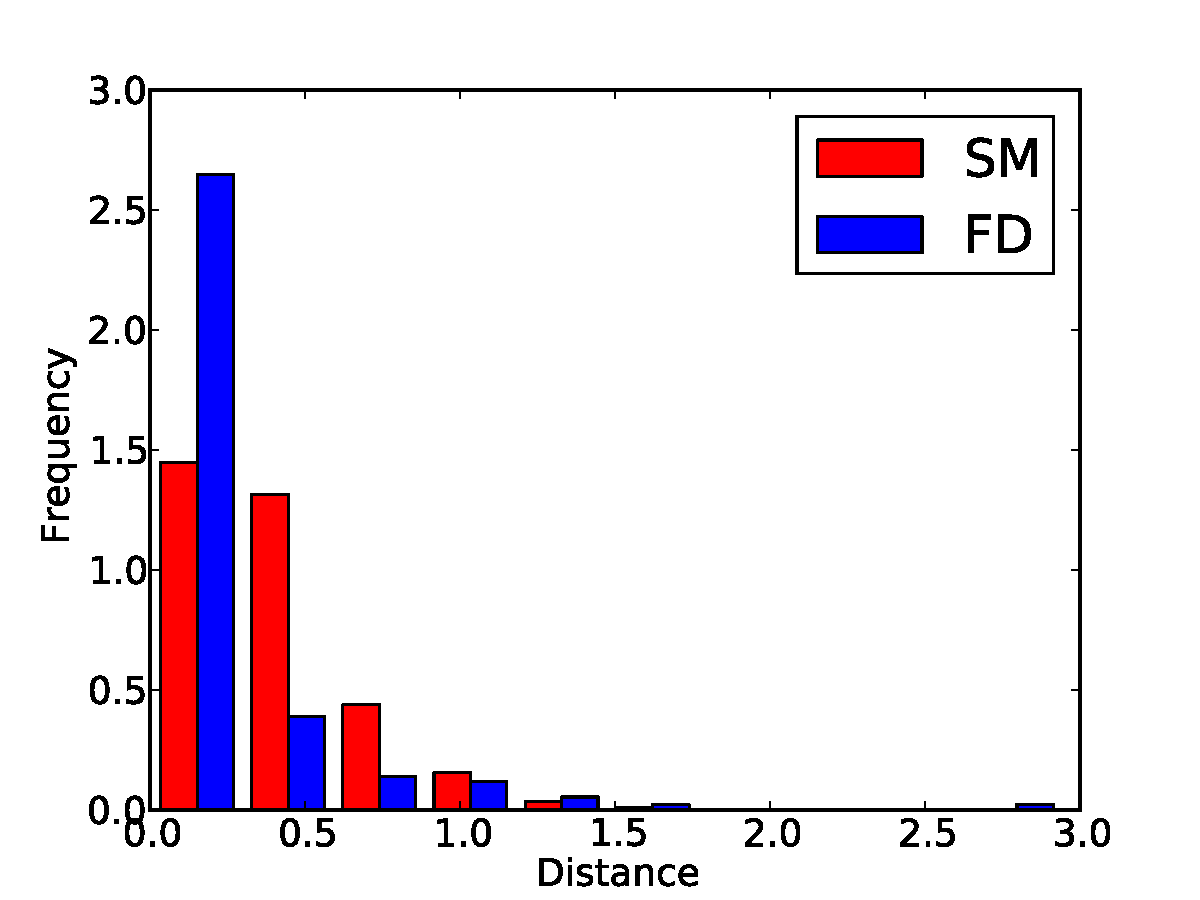
\includegraphics[width=1.7in]{ep_hist.pdf} 
&
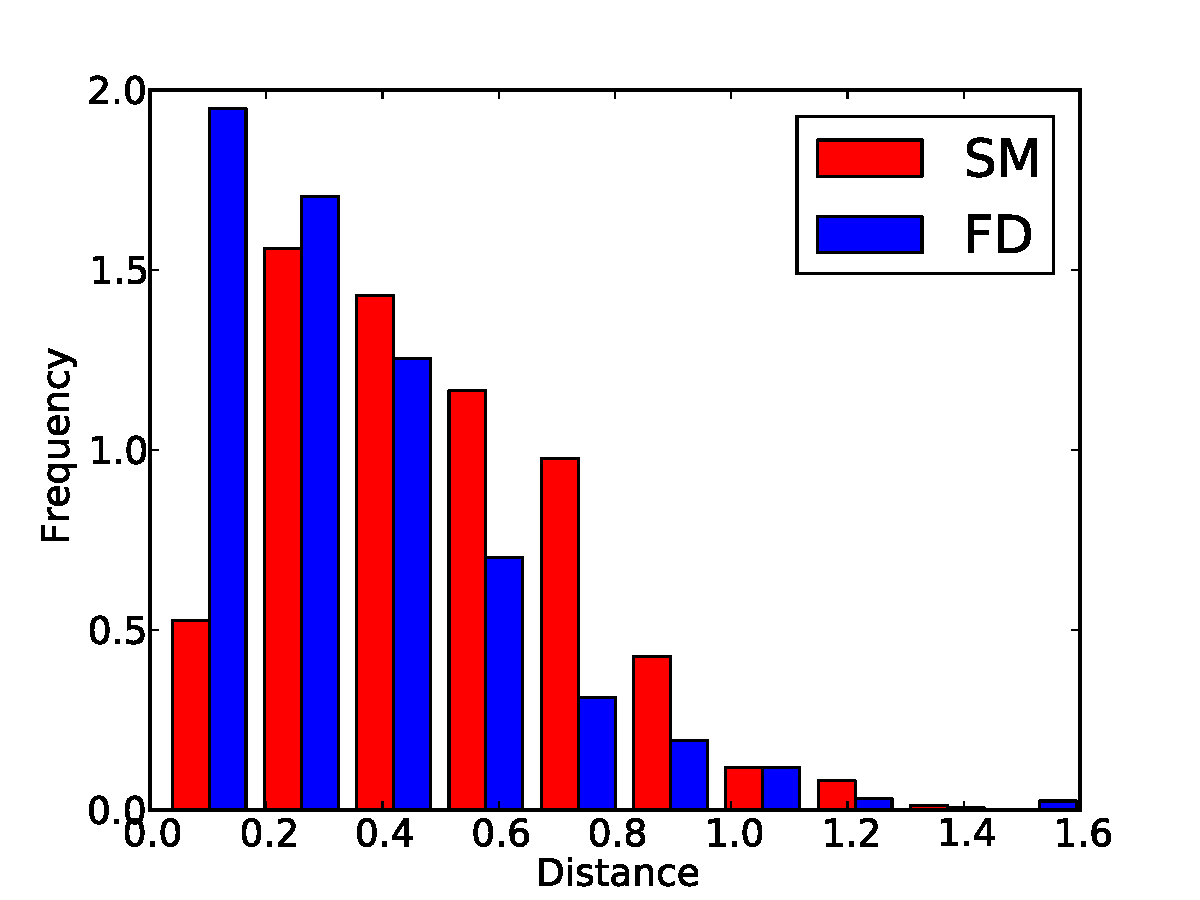
\includegraphics[width=1.7in]{wiki_hist.pdf} 
&
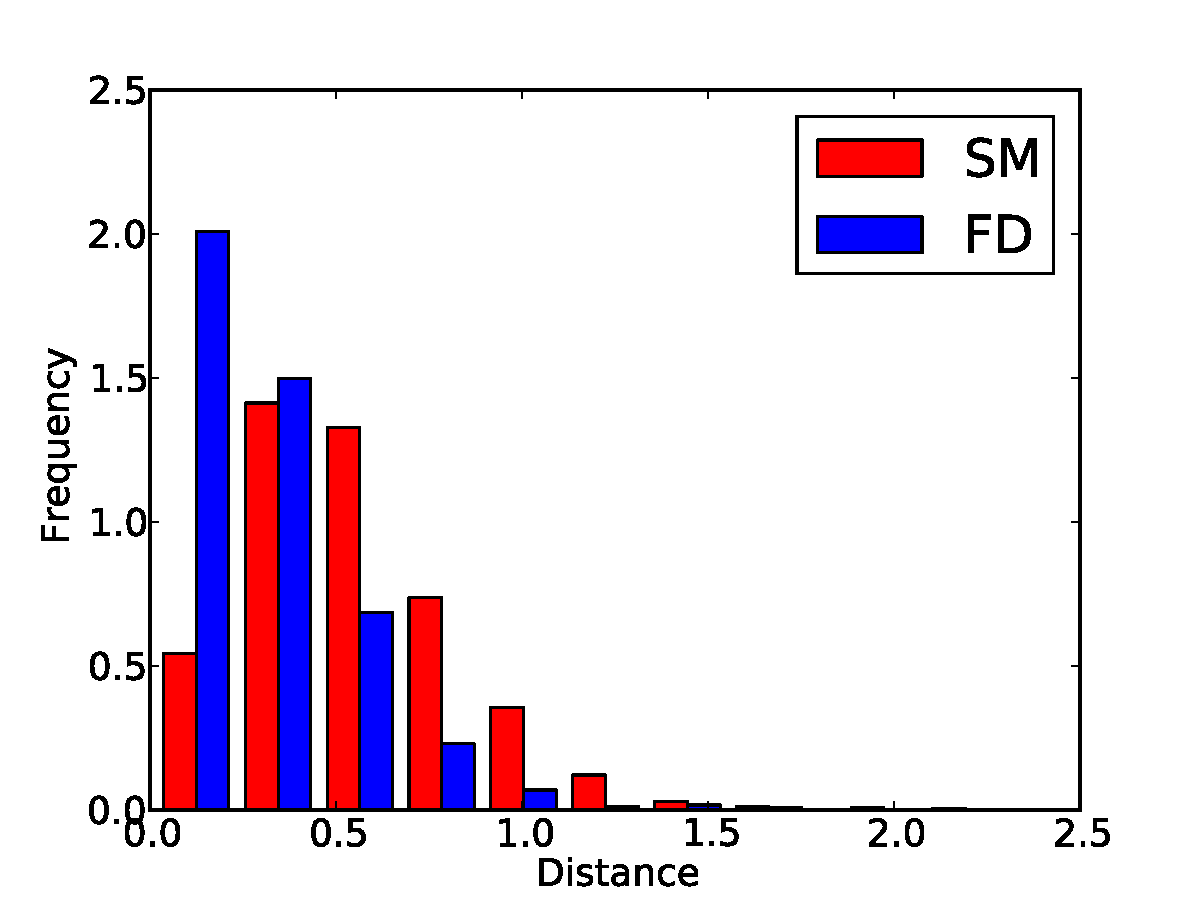
\includegraphics[width=1.7in]{slash_hist.pdf} \\
Epinions & Wikipedia & Slashdot
\end{tabular}}
\end{figure*}


\section{Conclusions} \label{sec:conclusions}
In this paper, we introduced a general model for structural balance
theory that can handle relation strengths and generalizes the
classical balance theory. Our theory builds on the hypothesis that
both the strong similarity and the strong dissimilarity in
relationships can cause stress in triads, but in different
directions. We showed that our theory naturally extends to cases
involving relationships with differing strength, allowing us to
represent strong and weak ties, as well as trust and distrust
relationships.  We showed that our theory can handle arbitrary
relation strengths drawn from a set of values with a total ordering.
Our notion of balance can also be mapped to triangular inequality when
relation strengths are modelled with metric distances.  Our extended
balance theory allows us to formally state the issue of convergence as
an optimization problem, in which individuals try to make the smallest
change in their relationships to resolve the inherent stress in the
triads that they are part of. This problem can be modeled as the
metric multidimensional scaling problem for which stress majorization
provides minimal solutions.

With the help of both stylized networks and an extensive experimental
study, we have shown that our theory can be used to effectively solve
the edge sign prediction problem. Its performance exceeds state of the
art for this problem. This is due to the fact that positive and
negative edges are mapped to a continuous range of strengths based on
the constraints provided by the other nodes. However, in contrast with
previous work, our method is aware of global constraints based on
balance which results in better results overall. We have shown that by
considering bi-directional edges as strong ties, the prediction
accuracy can be improved considerably for these edges. We provided
external validation that relation strength is correlated with rating
behavior, strong positive ties resulting in overall higher ratings and
string negative ties resulting in higher negative ties. Furthermore,
external validation shows that our convergence hypothesis correctly
predicts the negative edges that will becomes more positive over time
based on rating behavior. These edges are those that change sign by
our algorithm during the convergence process.  The algorithm is robust
to parameter choice and computationally feasible for sparse
graphs. Furthermore, we showed that the solutions provided by our
method provide a first step towards solving the harder {\it link
  prediction problem}.

We are investigating various avenues of future work. Our ability to
tailor the weights of different edges allows us to better incorporate
external data such as homophily of interests and level of supporting
evidence in trust relations into the framework. In such a framework,
edges with high homophily are less likely to change their sign from
positive to negative for example. Similarly, trust relations with a
great deal of past history are less likely to change, if this
information can be obtained from the underlying network.  Given such
measures have been shown to be effective in past work, incorporating
them can significantly improve prediction accuracy. There are also
alternate methods for translating asymmetric trust relations into
undirected trust strengths that present interesting avenues of
research. For example, the existence of distrust in any direction may be a
lot more diagnostic especially in trust relations based on reliability
and honesty. Different methods for modeling the directional trust
relations will provide the usual trade-off between supressing noise
and loosing information. Understanding how to address this problem and
when it makes a big different in performance is a topic of future
work.

Our method also has applications to many related problems like
clustering and link prediction, which we are currently
investigating. Our method also allows us to study and compare the
characteristics of existing networks towards balance such as the ratio
between positive and negative distances, and the distribution of
neutral edges. These measures can help us develop new insights into
the nature of adversarial relationships in different networks.

\begin{acks}
The authors would like to thank T. DuBois for sharing the implementation
details of the algorithms in~\cite{golbeck:distrust2011}.
\end{acks}


\bibliographystyle{acmsmall}
\bibliography{trust}

\end{document}


